\documentclass[11pt,oneside,openany]{book}
\usepackage[margin=1in,headheight=15pt]{geometry}
\usepackage[T1]{fontenc}
\usepackage{newtxtext,newtxmath}
\usepackage{microtype}
\usepackage{mathtools}
\usepackage{siunitx}
\usepackage{booktabs,longtable,tabularx,array,multirow}
\usepackage{graphicx,pdflscape}
\usepackage[dvipsnames,table]{xcolor}
\usepackage{tikz}
\usetikzlibrary{arrows.meta,calc,decorations.pathmorphing,positioning,shapes.geometric}
\usepackage{pgfplots}
\pgfplotsset{compat=1.18}
\usepackage[most]{tcolorbox}
\usepackage{enumitem}
\usepackage{fancyhdr}
\usepackage{titlesec}
\usepackage[round,authoryear]{natbib}
\usepackage{makeidx}
\usepackage{hyperref}
\usepackage[nameinlink,capitalise]{cleveref}
\makeindex

\definecolor{AtlasNavy}{HTML}{0B202C}
\definecolor{AtlasCyan}{HTML}{177E89}
\definecolor{AtlasAmber}{HTML}{D99028}
\definecolor{AtlasCoral}{HTML}{C95645}
\definecolor{AtlasMist}{HTML}{EDF5F3}
\hypersetup{colorlinks=true,linkcolor=AtlasNavy,citecolor=AtlasCyan,urlcolor=AtlasCoral,pdftitle={Line Atlas},pdfauthor={Tanmay Singh}}

\pagestyle{fancy}
\fancyhf{}
\fancyhead[L]{\small\nouppercase{\leftmark}}
\fancyhead[R]{\small Line Atlas}
\fancyfoot[C]{\thepage}
\renewcommand{\headrulewidth}{0.3pt}

\titleformat{\chapter}[display]
  {\normalfont\bfseries\color{AtlasNavy}}
  {\filleft\Large\chaptertitlename\ \thechapter}
  {1ex}{\titlerule\vspace{1.2ex}\Huge}
\titlespacing*{\chapter}{0pt}{-15pt}{36pt}

\newtcolorbox{conceptbox}[1][]{enhanced,breakable,colback=AtlasMist,colframe=AtlasCyan,boxrule=0.7pt,arc=0pt,title={#1},fonttitle=\bfseries,coltitle=AtlasNavy}
\newtcolorbox{cautionbox}[1][Caution]{enhanced,breakable,colback=AtlasAmber!8,colframe=AtlasAmber,boxrule=0.7pt,arc=0pt,title={#1},fonttitle=\bfseries,coltitle=AtlasNavy}
\newtcolorbox{workedexample}[1][Worked example]{enhanced,breakable,colback=white,colframe=AtlasNavy,boxrule=0.7pt,arc=0pt,title={#1},fonttitle=\bfseries,coltitle=white,colbacktitle=AtlasNavy}

\newcommand{\angstrom}{\text{\AA}}
\newcommand{\lineid}[1]{\textbf{#1}\index{#1}}
\newcommand{\ion}[2]{#1\,\textsc{#2}}
\newcommand{\forbidden}[1]{[\mathrm{#1}]}
\newcommand{\kms}{\si{\kilo\metre\per\second}}
\newcommand{\cmthree}{\si{\per\cubic\centi\metre}}
\newcommand{\Te}{T_{\mathrm e}}
\newcommand{\nelec}{n_{\mathrm e}}
\newcommand{\Nion}{N_{\mathrm{ion}}}
\DeclareMathOperator{\SNR}{S/N}


\title{\textbf{Line Atlas}\\[0.5em]\Large A Field Guide to Astrophysical Spectroscopy}
\author{Tanmay Singh}
\date{First edition --- \today}

\begin{document}
\hypersetup{pageanchor=false}
\begin{titlepage}
\pagecolor{AtlasNavy}
\color{white}
\vspace*{0.14\textheight}
{\Huge\bfseries LINE ATLAS\par}
\vspace{1.2em}
{\Large A Field Guide to Astrophysical Spectroscopy\par}
\vfill
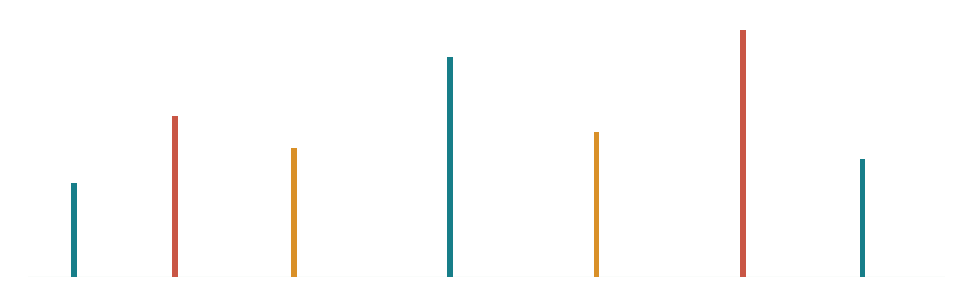
\begin{tikzpicture}[x=.96\textwidth,y=3.4cm]
  \draw[AtlasMist!30] (0,0)--(1,0);
  \foreach \x/\h/\c in {0.05/0.35/AtlasCyan,0.16/0.60/AtlasCoral,0.29/0.48/AtlasAmber,0.46/0.82/AtlasCyan,0.62/0.54/AtlasAmber,0.78/0.92/AtlasCoral,0.91/0.44/AtlasCyan}{
    \draw[line width=2pt,\c] (\x,0)--(\x,\h);
  }
\end{tikzpicture}
\vfill
{\large Tanmay Singh\par}
\vspace{0.5em}
{\small First edition --- \today\par}
\end{titlepage}
\nopagecolor
\color{black}

\hypersetup{pageanchor=true}
\frontmatter
\chapter*{Preface}
\addcontentsline{toc}{chapter}{Preface}

Spectroscopy turns small departures from a smooth continuum into measurements
of temperature, density, composition, radiation field, motion, and geometry.
That power comes with a practical difficulty: the meaning of a line is never
contained in its wavelength alone. A transition becomes useful only when its
atomic or molecular physics, excitation mechanism, optical depth, environment,
instrumental window, and degeneracies are considered together.

\emph{Line Atlas} is designed as a bridge between a line list and a textbook.
Each chapter develops the reasoning behind common measurements, while the
reference atlas provides a compact route back to individual transitions. The
companion website uses the same catalogue so that wavelength and redshift
questions can be explored interactively. Values in the atlas are starting
points, not substitutes for the critically evaluated source data and modelling
appropriate to a particular analysis.

This first edition emphasizes extragalactic work and the baryon cycle: H~II
regions, the neutral and molecular interstellar medium, stellar feedback, the
circumgalactic and intergalactic media, and active galactic nuclei. Radio,
infrared, ultraviolet, optical, and X-ray diagnostics are treated as connected
views of the same evolving gas.

\tableofcontents
\listoffigures
\listoftables

\mainmatter
\part{Reading Light}
\chapter{How to Read the Line Atlas}
\label{chap:foundations}

Spectroscopy is a translation problem.  The detector records counts as a
function of coordinate; the astronomer wants temperature, density, chemical
composition, radiation field, velocity, geometry, and evolutionary history.
A spectral transition connects those descriptions, but never by itself.  Its
meaning depends on how the relevant state was populated, how photons propagated,
which material shared the resolution element, and how the instrument transformed
the incoming radiation.  This opening chapter establishes the conventions used
throughout the atlas and a disciplined way to move from line identification to
physical inference.

\begin{conceptbox}[The central rule]
A line is evidence for a transition of a species.  Calling it a tracer of a
temperature, phase, or process is a model-dependent inference.  Preserve the
distinction between what the spectrum measures and what a physical model adds.
\end{conceptbox}

\section{The information carried by a line}

An isolated feature may provide several nearly independent observables:
\begin{enumerate}[label=\arabic*.]
  \item its centroid identifies a candidate transition and line-of-sight velocity;
  \item its integrated flux or equivalent width measures strength relative to a
        calibrated continuum;
  \item its width and profile encode thermal motion, turbulence, rotation,
        outflow, opacity, unresolved components, and the instrumental response;
  \item a resolved doublet or multiplet tests saturation, density, optical depth,
        and line identification;
  \item ratios to other transitions constrain excitation, ionization, attenuation,
        abundance, and the shape of the radiation field.
\end{enumerate}
These observables do not all imply the same spatial weighting.  Emissivity often
scales as a product of two densities, while absorption optical depth is linear in
the population of the lower state.  Bright emission therefore favors dense
structures; absorption can detect diffuse material along a long path.

For a transition between levels $u$ and $l$,
\begin{equation}
  h\nu_0 = E_u-E_l, \qquad \lambda_0 = \frac{c}{\nu_0}.
  \label{eq:foundation-transition}
\end{equation}
The rest coordinate is a laboratory property, whereas the observed coordinate is
altered by cosmological redshift and peculiar velocity.  To first order in
$v/c$, a small velocity displacement from a systemic wavelength obeys
\begin{equation}
  \Delta v \simeq c\,\frac{\lambda-\lambda_{\rm sys}}
                              {\lambda_{\rm sys}}.
\end{equation}
For high precision or large velocities one must state and use a relativistic
Doppler convention rather than mixing radio, optical, and relativistic velocity
definitions.

\begin{figure}[tbp]
\centering
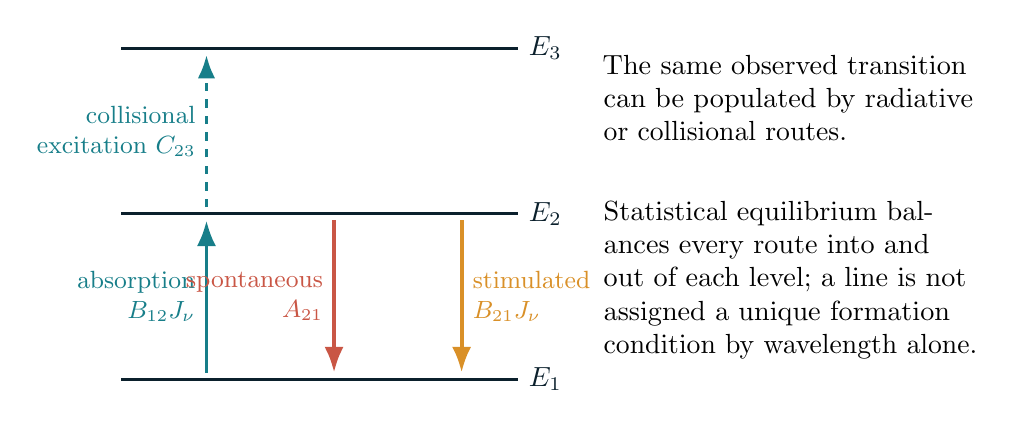
\begin{tikzpicture}[x=1.2cm,y=1.05cm,>=Latex]
  \foreach \y/\lab in {0/$E_1$,2/$E_2$,4/$E_3$}{
    \draw[AtlasNavy,line width=1pt] (0,\y)--(4.2,\y) node[right]{\lab};
  }
  \draw[->,AtlasCyan,line width=1.4pt] (0.9,0.08)--(0.9,1.92)
    node[midway,left,align=right,font=\small]{absorption\\$B_{12}J_\nu$};
  \draw[->,AtlasCoral,line width=1.4pt] (2.25,1.92)--(2.25,0.08)
    node[midway,left,align=right,font=\small]{spontaneous\\$A_{21}$};
  \draw[->,AtlasAmber,line width=1.4pt] (3.6,1.92)--(3.6,0.08)
    node[midway,right,align=left,font=\small]{stimulated\\$B_{21}J_\nu$};
  \draw[->,AtlasCyan,dashed,line width=1.2pt] (0.9,2.08)--(0.9,3.92)
    node[midway,left,align=right,font=\small]{collisional\\excitation $C_{23}$};
  \node[anchor=west,text width=4.8cm,align=left] at (5.0,3.4) {The same observed transition can be populated by radiative or collisional routes.};
  \node[anchor=west,text width=4.8cm,align=left] at (5.0,1.2) {Statistical equilibrium balances every route into and out of each level; a line is not assigned a unique formation condition by wavelength alone.};
\end{tikzpicture}
\caption{The principal bound--bound population and depopulation routes. The Einstein coefficients describe radiative transitions; collisional rates depend on collider density and the velocity-averaged cross section.}
\label{fig:line-processes}
\end{figure}


\section{Transition families}

The atlas groups lines by mechanism as well as wavelength.  The mechanism
determines the relevant selection rules, characteristic lifetime, and sensitivity
to density or radiation.

\begin{table}[tbp]
\centering
\caption{A physical taxonomy of common astronomical transitions.  The final
column gives a tendency, not an exclusive rule.}
\label{tab:transition-families}
\small
\begin{tabularx}{\textwidth}{@{}lXX X@{}}
\toprule
Family & Physical origin & Typical examples & Often constrains \\
\midrule
Permitted resonance & Electric-dipole transition from a populated lower level &
Ly$\alpha$, C\,IV, Mg\,II & column density, covering fraction, kinematics \\
Recombination & Cascades following radiative recombination &
H$\alpha$, H$\beta$, He\,II, radio recombination lines & ionizing-photon rate,
attenuation, emission measure \\
Forbidden or semi-forbidden & Long-lived state populated collisionally &
[O\,III], [S\,II], C\,III] & temperature, density, abundance, excitation source \\
Fine structure & Splitting within a ground electronic term &
[C\,II] $158\,\mu$m, [O\,I] $63\,\mu$m & gas cooling, collider density, PDR or
ionized-gas conditions \\
Rotational or inversion & Molecular rotation or tunnelling between configurations &
CO, HCN, NH$_3$ & molecular excitation, mass proxies, temperature, dense gas \\
Hyperfine & Coupling of nuclear and electronic angular momentum &
H\,I 21 cm, OH 18 cm & neutral gas, spin temperature, magnetic field \\
Inner-shell or nuclear & Atomic K-shell rearrangement or nuclear decay &
Fe K$\alpha$, 511 keV, $^{26}$Al & irradiation, compact objects, nucleosynthesis \\
\bottomrule
\end{tabularx}
\end{table}

The adjective ``forbidden'' means forbidden by the leading electric-dipole
selection rules, not impossible.  In a sufficiently low-density plasma the upper
state survives long enough to radiate.  At high collider density, de-excitation
may occur collisionally before a photon escapes; this is the origin of critical
density diagnostics.  Likewise, a molecular line with a large dipole moment is
not automatically a unique dense-gas tracer: radiative trapping, subthermal
excitation, abundance, infrared pumping, and beam dilution all matter.

\section{Reading species and transition labels}

Astronomical ion notation counts the neutral atom as stage I, so O\,VI is
O$^{5+}$ rather than O$^{6+}$.  Square brackets denote a forbidden transition,
as in [O\,III] $\lambda5007$; a closing bracket alone conventionally marks a
semi-forbidden transition, as in C\,III].  A wavelength following $\lambda$ is
usually in Angstrom unless another unit is shown.  Molecular notation instead
specifies rotational, vibrational, inversion, or hyperfine quantum numbers, for
example CO($J=1\!\rightarrow\!0$) or H$_2$ 1--0 S(1).

The ionization threshold needed to create an ion is not the energy of the listed
line.  The former describes removal of an electron; the latter is the separation
of two bound levels.  Confusing them can lead to incorrect claims about the
hardness of the radiation required to produce a feature.  Ion fractions also
depend on recombination and charge exchange, not only threshold energy
\citep{OsterbrockFerland2006,Draine2011}.

\section{Coordinates, units, and conventions}

\subsection{Vacuum and standard air wavelengths}

This edition stores atomic wavelengths in vacuum unless an entry explicitly says
otherwise.  Familiar ground-based optical names often use standard air values:
H$\alpha$ is commonly called $6562.8$~\AA\ in air but is approximately
$6564.6$~\AA\ in vacuum.  The difference is scientifically significant for
precision velocities.  Conversion depends on a refractive-index prescription and
its validity range, so an analysis must record both the input convention and the
formula used.  NIST distinguishes observed and Ritz wavelengths and documents
the medium used by its tabulations \citep{nist-asd}.

\subsection{Use the native coordinate}

At centimetre and millimetre wavelengths, observers tune to a rest frequency and
should retain it rather than relying on a rounded wavelength conversion.  X-ray
features are often reported in energy, while optical and ultraviolet features are
normally reported in wavelength.  The equivalent representations obey
\begin{equation}
  E = h\nu = \frac{hc}{\lambda},
  \qquad
  \left|\frac{\Delta E}{E}\right|
  =\left|\frac{\Delta\nu}{\nu}\right|
  =\left|\frac{\Delta\lambda}{\lambda}\right|
\end{equation}
for small intervals.  Significant digits should follow the authoritative
laboratory uncertainty and component definition, not the numerical precision of
a unit conversion.

\subsection{Flux-density transformations}

Flux density per unit frequency and per unit wavelength are related by a Jacobian,
\begin{equation}
 f_\lambda = f_\nu\left|\frac{\mathrm d\nu}{\mathrm d\lambda}\right|
 =f_\nu\frac{c}{\lambda^2},
 \qquad \lambda f_\lambda=\nu f_\nu.
\end{equation}
A spectrum that is flat in $f_\nu$ is therefore not flat in $f_\lambda$.
Integrated line flux remains an energy flux after integrating over a consistently
defined coordinate, but equivalent widths and continuum slopes must retain their
coordinate convention \citep{RybickiLightman1979}.

\section{From identification to inference}

A credible line identification is a network of consistency checks rather than a
nearest-wavelength match.  The following sequence is used throughout this book.

\begin{enumerate}[label=\textbf{Step \arabic*:},leftmargin=*]
  \item \textbf{Calibrate the coordinate.} Establish the wavelength solution,
  barycentric or local-standard-of-rest correction, air/vacuum convention, and
  uncertainty.
  \item \textbf{Generate candidate transitions.} Use the allowed redshift range,
  spectral coverage, expected source class, and a current laboratory database.
  \item \textbf{Demand companions.} Search for doublet partners, other members of
  the same series, adjacent ionization stages, and physically expected continuum
  features.
  \item \textbf{Test the profile.} Compare component velocities and widths after
  applying the line-spread function; inspect blends, sky residuals, detector
  defects, and telluric absorption.
  \item \textbf{Separate measurement from model.} Report flux, equivalent width,
  centroid, width, covariance, and limits before translating them into abundance,
  density, temperature, or mass.
  \item \textbf{Stress-test alternatives.} Vary continuum placement, component
  count, attenuation law, atomic data, ionization mechanism, geometry, and priors.
\end{enumerate}

\begin{cautionbox}[A non-detection is not zero]
A non-detection constrains a line only through the noise model, assumed profile,
searched velocity interval, and selection procedure.  Report an upper limit with
its confidence convention and assumed width; preserve the likelihood or sensitivity
curve when it will enter population inference.
\end{cautionbox}

\section{How each atlas entry is constructed}

Each generated entry records an operational rest coordinate, physical mechanism,
common environments, useful tracers, an indicative temperature regime, density
guidance, diagnostic companions, observing cautions, and source keys.  The source
hierarchy is deliberate: critically evaluated atomic or molecular databases supply
rest data; primary papers and reviews supply interpretation; observatory documents
supply current instrumental limits.  The prose is a guide to discovery, not a
replacement for a live database query or a forward model.

The phrase ``temperature regime'' is especially easy to overread.  A quoted
collisional-ionization-equilibrium peak is an orientation point.  Photoionization,
non-equilibrium cooling, shocks, mixing, charge exchange, optical depth, and an
unresolved multiphase sightline can produce the same ion under different kinetic
conditions.  Similarly, a critical density depends on the collider and temperature;
an effective excitation density also depends on opacity and column.

\section{A compact reporting standard}

For a result to be reproducible, a line measurement should state at least:
\begin{itemize}
  \item transition and component, adopted rest coordinate, source database and
        version, and air/vacuum convention;
  \item reference frame, redshift or velocity convention, and systemic-redshift
        uncertainty;
  \item instrument, configuration, resolving power, sampling, aperture, and
        line-spread-function treatment;
  \item continuum model, integration or fitting window, blend model, and
        attenuation correction;
  \item flux, equivalent width, centroid, width, uncertainties and covariance, or
        the complete upper-limit prescription;
  \item physical model, radiation field, abundance pattern, atomic or molecular
        data, priors, and sensitivity tests used for interpretation.
\end{itemize}

This standard may look longer than a table cell, but most fields belong in a
machine-readable companion product.  The purpose of the atlas is to make those
dependencies visible early, before a memorable line name hardens into an
overconfident physical claim.

% Line Atlas chapter draft.
% Suggested dependencies: amsmath, amssymb, bm, siunitx, booktabs,
% tabularx, tikz, pgfplots, xcolor, hyperref. Set \pgfplotsset{compat=1.18}.
% Citation keys are defined in line_atlas_references.bib.

\chapter{Radiation, Matter, and the Making of a Spectral Line}
\label{chap:radiative-transfer-foundations}
\chaptermark{Radiation, Matter, and Spectral Lines}

Spectral lines are not labels pasted onto otherwise featureless spectra.  They are
the observable end point of a chain of physical events: particles are placed in
quantum states, photons are created or destroyed, radiation propagates through a
structured medium, and an instrument averages the emerging field over angle,
wavelength, and time.  A line atlas is most useful when every entry can be read in
both directions along this chain.  From an observed feature one would like to infer
density, temperature, abundance, velocity, and radiation field; from a proposed
physical model one would like to predict a measurable flux profile.

This chapter establishes the vocabulary needed for both directions.  It emphasizes
the assumptions hidden in familiar formulae and the combinations of quantities that
spectra actually constrain.  More complete treatments are given by
\citet{RybickiLightman1979}, \citet{Mihalas1978},
\citet{OsterbrockFerland2006}, and \citet{Draine2011}.

\section{What a spectrograph measures}

The fundamental radiometric quantity is the specific intensity
$I_\nu(\boldsymbol{x},\hat{\boldsymbol{n}},t)$, defined so that the energy crossing an
area element $\mathrm{d}A$ in time $\mathrm{d}t$, within solid angle
$\mathrm{d}\Omega$ and frequency interval $\mathrm{d}\nu$, is
\begin{equation}
 \mathrm{d}E = I_\nu\cos\theta\,\mathrm{d}A\,\mathrm{d}t\,
              \mathrm{d}\Omega\,\mathrm{d}\nu .
 \label{eq:rt-intensity-definition}
\end{equation}
Unlike flux, intensity is conserved along a ray in empty Euclidean space.  The
monochromatic flux is the first angular moment,
\begin{equation}
 F_\nu = \int_{4\pi} I_\nu(\hat{\boldsymbol{n}})\cos\theta\,\mathrm{d}\Omega ,
 \qquad
 J_\nu = \frac{1}{4\pi}\int_{4\pi}I_\nu\,\mathrm{d}\Omega ,
 \label{eq:rt-moments}
\end{equation}
where $J_\nu$ is the mean intensity.  An unresolved source at luminosity distance
$D_L$ is normally reported through a flux density $f_\nu$ or $f_\lambda$.  The two
are not numerically interchangeable:
\begin{equation}
 f_\lambda = f_\nu\left|\frac{\mathrm{d}\nu}{\mathrm{d}\lambda}\right|
 = f_\nu\frac{c}{\lambda^2},
 \qquad \lambda f_\lambda=\nu f_\nu .
 \label{eq:fnu-flambda}
\end{equation}
This Jacobian is the reason that a spectrum flat in $f_\nu$ slopes as
$\lambda^{-2}$ in $f_\lambda$.

For a source at redshift $z$, $\nu_{\rm obs}=\nu_{\rm em}/(1+z)$ and
$\lambda_{\rm obs}=(1+z)\lambda_{\rm em}$.  Specific intensity obeys the
Liouville invariant $I_\nu/\nu^3$ along a null geodesic in the absence of
interactions.  Consequently surface brightness dims as $(1+z)^{-4}$ after
integrating over frequency.  Line luminosity and observed integrated line flux are
related by
\begin{equation}
 F_{\rm line}=\int f_\lambda\,\mathrm{d}\lambda_{\rm obs}
             =\frac{L_{\rm line}}{4\pi D_L^2}.
 \label{eq:line-flux-luminosity}
\end{equation}
No extra factor of $(1+z)$ belongs in this bolometric line relation; such factors
enter relations between spectral densities or between velocity-integrated radio
brightness and luminosity.

\paragraph{Definition: line profile.}
The line profile $\phi(\nu)$ is a probability density in frequency, normalized as
$\int\phi(\nu)\,\mathrm{d}\nu=1$.  It therefore has units of inverse frequency.
Omitting this unit is a common route to dimensionally incorrect opacity formulae.

\section{The transfer equation and its formal solution}

Along path length $s$, emission adds radiation and extinction removes it:
\begin{equation}
 \frac{\mathrm{d}I_\nu}{\mathrm{d}s}=j_\nu-\alpha_\nu I_\nu,
 \label{eq:transfer-dimensional}
\end{equation}
where $j_\nu$ is the emission coefficient per steradian and $\alpha_\nu$ is the
extinction coefficient.  True absorption and scattering may both contribute to
$\alpha_\nu$; only true absorption transfers radiant energy to internal energy.
Define optical depth increasing away from the observer by
$\mathrm{d}\tau_\nu=\alpha_\nu\mathrm{d}s$ and source function
$S_\nu=j_\nu/\alpha_\nu$.  For a slab of total optical depth $\tau_\nu$, the
emergent intensity is
\begin{equation}
 I_\nu(0)=I_\nu(\tau_\nu)e^{-\tau_\nu}
 +\int_0^{\tau_\nu} S_\nu(t)e^{-t}\,\mathrm{d}t .
 \label{eq:formal-solution}
\end{equation}
For a homogeneous slab this becomes
\begin{equation}
 I_{\nu,\rm out}=I_{\nu,\rm bg}e^{-\tau_\nu}
                 +S_\nu\left(1-e^{-\tau_\nu}\right).
 \label{eq:homogeneous-slab}
\end{equation}
Equation~\eqref{eq:homogeneous-slab} is one of the most useful diagnostic equations
in spectroscopy.  A feature appears in emission when the line source function
exceeds the incident background intensity and in absorption when it is smaller.
Thus ``emission line'' and ``absorption line'' describe contrast, not an intrinsic
property of a transition.

When the material is in local thermodynamic equilibrium (LTE), detailed balance
gives $S_\nu=B_\nu(T)$, the Planck function.  LTE requires collisional processes to
establish local level populations, but does not require the radiation field to be a
blackbody.  In a stratified, optically thick atmosphere with a slowly varying source
function, the Eddington--Barbier approximation gives
$I_\nu(0,\mu)\simeq S_\nu(\tau_\nu=\mu)$, where
$\mu=\cos\theta$.  We therefore see different physical depths at different
frequencies: high-opacity line cores form closer to the surface than adjacent
continuum.

\subsection{Absorption, stimulated emission, and spontaneous emission}

Consider lower and upper states $l$ and $u$, populations $n_l$ and $n_u$, and
statistical weights $g_l$ and $g_u$.  Einstein coefficients describe absorption
($B_{lu}$), stimulated emission ($B_{ul}$), and spontaneous emission ($A_{ul}$).
Their thermodynamic relations are
\begin{equation}
 g_lB_{lu}=g_uB_{ul},\qquad
 A_{ul}=\frac{2h\nu_0^3}{c^2}B_{ul}.
 \label{eq:einstein-relations}
\end{equation}
For complete redistribution with the same normalized line profile for absorption
and emission,
\begin{align}
 j_\nu^{\rm line} &= \frac{h\nu_0}{4\pi}n_uA_{ul}\phi(\nu),\\
 \alpha_\nu^{\rm line} &= \frac{h\nu_0}{4\pi}
             \left(n_lB_{lu}-n_uB_{ul}\right)\phi(\nu).
 \label{eq:line-j-alpha}
\end{align}
The negative stimulated-emission term matters at radio wavelengths and in population
inversions.  It should not be silently discarded merely because spontaneous emission
dominates a particular optical application.

The absorption oscillator strength $f_{lu}$ is related to the frequency-integrated
cross section by
\begin{equation}
 \int\sigma_\nu\,\mathrm{d}\nu=\frac{\pi e^2}{m_ec}f_{lu},
 \qquad
 \sigma_\nu=\frac{\pi e^2}{m_ec}f_{lu}\phi(\nu).
 \label{eq:oscillator-strength-cross-section}
\end{equation}
Oscillator strengths are dimensionless atomic data.  Their uncertainty can dominate
an abundance measurement even when the spectrum has extremely high signal-to-noise.

\section{Population equations: LTE and statistical equilibrium}

In LTE, excitation follows the Boltzmann relation,
\begin{equation}
 \frac{n_u}{n_l}=\frac{g_u}{g_l}
 \exp\!\left[-\frac{E_u-E_l}{kT}\right],
 \label{eq:boltzmann-populations}
\end{equation}
and adjacent ionization stages follow the Saha equation,
\begin{equation}
 \frac{n_{i+1}n_e}{n_i}=
 \frac{2}{\lambda_e^3}\frac{U_{i+1}(T)}{U_i(T)}
 \exp\!\left(-\frac{\chi_i}{kT}\right),
 \qquad
 \lambda_e=\frac{h}{\sqrt{2\pi m_ekT}}.
 \label{eq:saha}
\end{equation}
Here $U_i$ is a partition function and $\chi_i$ the ionization potential.  Nebulae,
diffuse clouds, and the circumgalactic medium are generally not in LTE.  Their level
populations instead satisfy statistical equilibrium,
\begin{equation}
 \sum_{j\ne i}n_jP_{ji}=n_i\sum_{j\ne i}P_{ij},
 \qquad \sum_i n_i=n_{\rm species},
 \label{eq:statistical-equilibrium}
\end{equation}
where each $P_{ij}$ may contain radiative, electron-impact, neutral-impact,
recombination, charge-exchange, or chemical rates.

For an optically thin two-level ion excited by electron collisions, neglecting
stimulated terms,
\begin{equation}
 \frac{n_u}{n_l}=\frac{n_eq_{lu}}{A_{ul}+n_eq_{ul}},
 \qquad n_{\rm crit}=\frac{A_{ul}}{q_{ul}}.
 \label{eq:two-level-atom}
\end{equation}
At $n_e\ll n_{\rm crit}$, each excitation is usually followed by a photon, so the
volume emissivity scales approximately as $n_en_l$.  At
$n_e\gg n_{\rm crit}$, collisions de-excite the upper state and the line no longer
grows quadratically.  For a multilevel atom the denominator must include every
downward collider and radiative branch,
\begin{equation}
 n_{{\rm crit},u}=\frac{\sum_{l<u}A_{ul}}
 {\sum_{j\ne u}\sum_c n_cq^{(c)}_{uj}/n_e},
 \label{eq:multilevel-critical-density}
\end{equation}
or, more transparently, one quotes a collider-specific critical density
$n_{{\rm crit},c}=\sum A_{ul}/\sum q^{(c)}_{uj}$.  Tabulated critical densities are
therefore temperature dependent and are not universal constants of a line.

\paragraph{Caveat: critical density is not a hard boundary.}
Line emissivity changes smoothly around $n_{\rm crit}$.  Radiative trapping lowers
the effective spontaneous escape rate, while continuum pumping raises levels without
collisions.  A measured density-sensitive ratio should be interpreted with a full
multilevel model when optical depth, fluorescence, or several colliders matter.

\section{Why lines have width and shape}

The natural profile of an isolated damped transition is Lorentzian.  Thermal and
microturbulent Doppler shifts produce a Gaussian core.  Their convolution is the
Voigt profile,
\begin{equation}
 \phi(\nu)=\frac{H(a,u)}{\sqrt{\pi}\Delta\nu_D},\quad
 u=\frac{\nu-\nu_0}{\Delta\nu_D},\quad
 a=\frac{\Gamma}{4\pi\Delta\nu_D},
 \label{eq:voigt-profile}
\end{equation}
where $\Gamma$ is the total damping rate and
\begin{equation}
 \Delta\nu_D=\frac{\nu_0b}{c},\qquad
 b^2=\frac{2kT}{m}+b_{\rm nt}^2.
 \label{eq:doppler-b}
\end{equation}
The Doppler parameter $b$ is related to a Gaussian velocity dispersion by
$b=\sqrt{2}\sigma_v$ and to full width at half maximum by
$\mathrm{FWHM}=2\sqrt{\ln2}\,b\simeq1.665b$.  Mixing these conventions can bias
temperatures by a factor of two.

If two ions share the same temperature and nonthermal broadening, their measured
widths obey
\begin{equation}
 b_1^2-b_2^2=2kT\left(\frac{1}{m_1}-\frac{1}{m_2}\right).
 \label{eq:two-ion-temperature}
\end{equation}
The method is powerful only when the profiles are demonstrably co-spatial and the
instrumental line-spread function has been removed.  Unresolved component structure
usually mimics nonthermal broadening.

\begin{figure}[tbp]
\centering
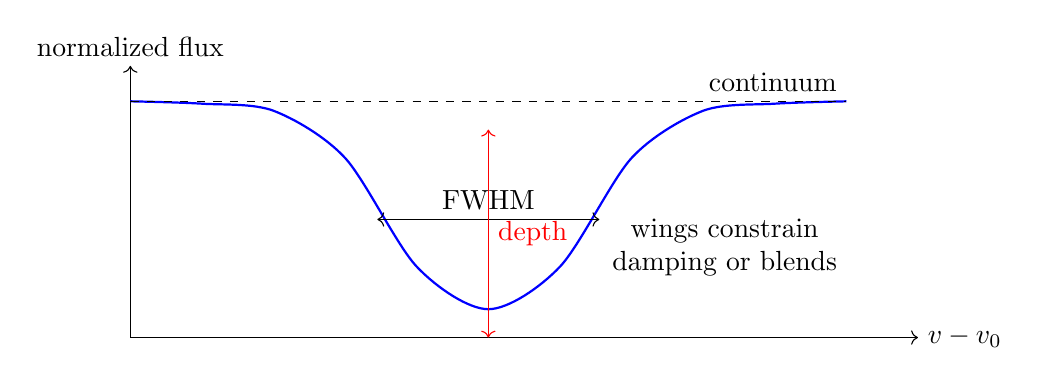
\begin{tikzpicture}[x=0.075\linewidth,y=3.0cm]
  \draw[->] (0,0) -- (11,0) node[right] {$v-v_0$};
  \draw[->] (0,0) -- (0,1.15) node[above] {normalized flux};
  \draw[thick,blue]
    plot[smooth] coordinates {(0,1.0) (1,0.99) (2,0.96) (3,0.76)
    (4,0.30) (5,0.12) (6,0.30) (7,0.76) (8,0.96) (9,0.99) (10,1.0)};
  \draw[dashed] (0,1) -- (10,1) node[above left] {continuum};
  \draw[<->] (3.45,0.50) -- (6.55,0.50)
    node[midway,above] {FWHM};
  \draw[<->,red] (5,0) -- (5,0.88)
    node[midway,right] {depth};
  \node[align=center] at (8.3,0.38) {wings constrain\\damping or blends};
\end{tikzpicture}
\caption{Original schematic for a normalized absorption profile.  A production
version can overlay intrinsic, instrument-convolved, and sampled profiles.  The
equivalent width is the area between the continuum and profile, not simply depth
times FWHM.}
\label{fig:line-profile-anatomy}
\end{figure}

Macroscopic velocity gradients produce profiles that cannot be represented by a
single Voigt function.  Rotation can create a double-horned integrated profile;
accelerating outflows can form P-Cygni profiles; self-absorption can split an
otherwise single emission peak.  The measured spectrum is finally convolved with
the instrument line-spread function $L$ and integrated over detector pixels:
\begin{equation}
 f_i=\int_{\Delta\lambda_i}
       \left[f_{\lambda,\rm true}*L\right](\lambda)\,
       R_i(\lambda)\,\mathrm{d}\lambda,
 \label{eq:forward-instrument}
\end{equation}
where $R_i$ includes pixel response.  Deconvolving noisy data is unstable; forward
convolution of a physical model is normally preferable.

\section{Optical depth, equivalent width, and the curve of growth}

For a column density $N_l$ in the lower state, a Doppler-broadened absorption line
has central optical depth
\begin{equation}
 \tau_0=\frac{\sqrt{\pi}e^2}{m_ec}
         \frac{f_{lu}\lambda_0N_l}{b}
 =1.497\times10^{-15}
 \frac{N_l}{\mathrm{cm}^{-2}}
 \frac{f_{lu}(\lambda_0/\text{\AA})}{b/(\mathrm{km\,s^{-1}})}.
 \label{eq:line-center-optical-depth}
\end{equation}
The rest-frame equivalent width of an absorption line is
\begin{equation}
 W_0=\int\left(1-\frac{F_\lambda}{F_c}\right)
      \mathrm{d}\lambda_{\rm rest},
 \qquad W_{\rm obs}=(1+z)W_0.
 \label{eq:equivalent-width}
\end{equation}
For optically thin absorption,
\begin{equation}
 W_0=\frac{\pi e^2}{m_ec^2}N_lf_{lu}\lambda_0^2,
 \label{eq:linear-cog}
\end{equation}
independent of $b$.  As the core saturates, increasing $N_l$ mostly broadens the
black portion of the line and $W$ grows only roughly as $b\sqrt{\ln \tau_0}$.
At still larger columns, Lorentzian damping wings cause
$W\propto N_l^{1/2}$.  These are the linear, saturated, and damping regimes of the
curve of growth.

\begin{figure}[tbp]
\centering
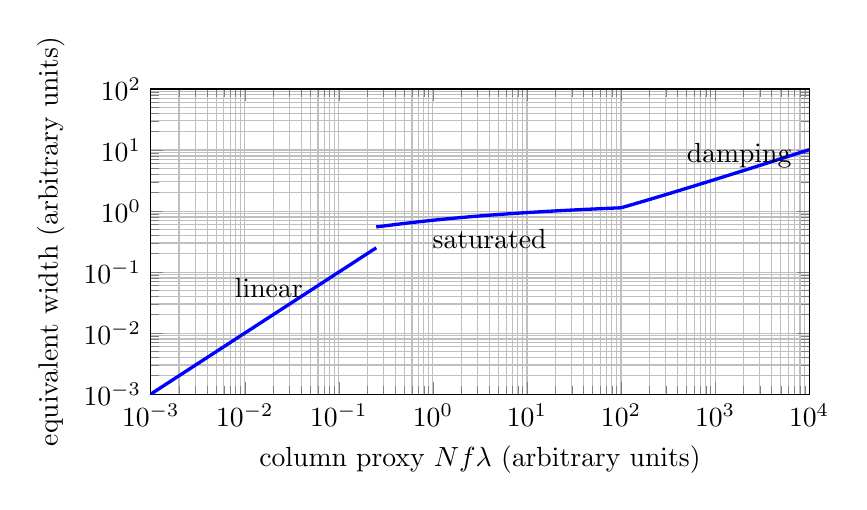
\begin{tikzpicture}
\begin{loglogaxis}[
 width=0.82\linewidth,height=0.45\linewidth,
 xlabel={column proxy $Nf\lambda$ (arbitrary units)},
 ylabel={equivalent width (arbitrary units)},
 xmin=1e-3,xmax=1e4,ymin=1e-3,ymax=1e2,
 grid=both,legend style={draw=none,fill=none},
]
 \addplot[very thick,blue,domain=0.001:0.25,samples=40] {x};
 \addplot[very thick,blue,domain=0.25:100,samples=80]
   {0.25+0.36*sqrt(ln(1+4*x))};
 \addplot[very thick,blue,domain=100:10000,samples=60]
   {0.25+0.36*sqrt(ln(401))+0.10*(sqrt(x)-10)};
 \node at (axis cs:0.018,0.055) {linear};
 \node at (axis cs:4,0.35) {saturated};
 \node at (axis cs:1800,8) {damping};
\end{loglogaxis}
\end{tikzpicture}
\caption{Pedagogical curve-of-growth concept generated entirely with PGFPlots.
The plotted interpolation is schematic, not a substitute for evaluating a Voigt
profile.  A final atlas could add families of curves for several Doppler parameters.}
\label{fig:curve-of-growth-concept}
\end{figure}

\subsection{Worked example: is a Ly\texorpdfstring{$\alpha$}{-alpha} absorber optically thin?}

Take H\,I Ly$\alpha$ with $f=0.4164$ and
$\lambda_0=1215.67$~\AA.  For
$N_{\mathrm{H\,I}}=10^{14}\,\mathrm{cm}^{-2}$ and
$b=20\,\mathrm{km\,s^{-1}}$, equation~\eqref{eq:line-center-optical-depth}
gives
\begin{equation}
 \tau_0\simeq1.497\times10^{-15}
 \frac{10^{14}\times0.4164\times1215.67}{20}\simeq3.8.
\end{equation}
The line is already saturated at its center, even though its neutral-hydrogen column
is modest by interstellar standards.  Applying the optically thin equivalent-width
formula would underestimate $N_{\mathrm{H\,I}}$.  Higher Lyman-series transitions,
a curve-of-growth analysis, or a forward Voigt-profile fit are needed.  A formally
excellent single-component fit can still be wrong if narrow components are hidden by
the line-spread function.

\section{Emission measure, surface brightness, and luminosity}

For optically thin recombination radiation, the line emissivity integrated over
solid angle is often written
\begin{equation}
 \epsilon_{ul}=h\nu_{ul}n_en_{i+1}\alpha^{\rm eff}_{ul}(T),
 \qquad
 L_{ul}=\int_V\epsilon_{ul}\,\mathrm{d}V.
 \label{eq:recombination-emissivity}
\end{equation}
The effective recombination coefficient includes cascades that feed the upper state.
The surface brightness scales with emission measure,
\begin{equation}
 {\rm EM}=\int n_en_p\,\mathrm{d}\ell,
 \qquad
 I_{ul}=\frac{h\nu_{ul}}{4\pi}
 \int n_en_p\alpha^{\rm eff}_{ul}(T)\,\mathrm{d}\ell.
 \label{eq:emission-measure}
\end{equation}
Because EM weights density squared, dense clumps dominate emission.  Absorption
columns weight density linearly.  Combining emission and absorption is therefore a
way to constrain clumping, but only if the two measurements sample the same gas.

Collisionally excited forbidden lines have low-density emissivity
\begin{equation}
 \epsilon_{ul}\simeq n_en(X^i)q_{lu}(T)h\nu_{ul}
 \frac{A_{ul}}{\sum_k A_{uk}},
 \label{eq:cel-emissivity}
\end{equation}
with excitation coefficient
\begin{equation}
 q_{lu}(T)=\frac{8.629\times10^{-6}}{g_lT^{1/2}}
 \Upsilon_{lu}(T)\exp\!\left(-\frac{\Delta E}{kT}\right)
 \quad \mathrm{cm^3\,s^{-1}}.
 \label{eq:collisional-rate-coefficient}
\end{equation}
The effective collision strength $\Upsilon$ varies more gently with temperature
than the exponential.  This strong temperature sensitivity makes auroral-to-nebular
ratios valuable thermometers and also makes inferred abundances sensitive to
unresolved temperature structure.

\subsection{Worked example: a density-sensitive doublet}

Suppose two lines arise from metastable levels with different $A/q$ values but close
excitation energies.  Their ratio can be approximated schematically by
\begin{equation}
 R(n_e)=R_0\frac{1+n_e/n_{{\rm crit},2}}
                     {1+n_e/n_{{\rm crit},1}}.
 \label{eq:doublet-density-schematic}
\end{equation}
At densities below both critical densities, $R\rightarrow R_0$ and the diagnostic
loses leverage.  At densities above both, it approaches another asymptote and again
loses leverage.  The ratio is informative primarily between the two critical
densities.  An observer should report an upper or lower limit when a measured ratio
lies near an asymptote, rather than quote a spuriously precise density.

\section{Resonant scattering, escape, and redistribution}

Resonance lines such as Ly$\alpha$, C\,IV, Mg\,II, and Na\,I D may scatter many
times before escape.  Scattering conserves photon number only in the idealized
absence of dust absorption, collisional de-excitation, conversion to other lines, or
escape outside the aperture.  A simple escape-probability approximation replaces
$A_{ul}$ by $\beta(\tau)A_{ul}$, where for a static slab one rough choice is
\begin{equation}
 \beta(\tau)\simeq\frac{1-e^{-\tau}}{\tau}.
 \label{eq:escape-probability}
\end{equation}
This captures the limiting trends but not detailed frequency diffusion or geometry.
At large optical depth, photons escape through frequency excursions into the wings;
bulk velocity and dust geometry can then shape the emergent profile more strongly
than the intrinsic production spectrum.

\paragraph{Interpretive caution.}
The centroid of a resonant emission line need not equal the systemic velocity, and
its integrated flux need not measure only the production rate.  A spatially extended
halo may be composed largely of photons created in the central region and scattered
into the line of sight.  Conversely, a narrow spectroscopic aperture may classify
scattered photons as ``destroyed'' even when they merely emerge elsewhere.

\section{A hierarchy of modeling assumptions}

Line interpretation should state its rung on the following hierarchy:
\begin{enumerate}
 \item \textbf{Optically thin emissivity or absorption.}  Photons interact at most
 once; geometry enters only through an integral of density or density squared.
 \item \textbf{One-zone statistical equilibrium.}  Level populations respond to a
 specified temperature, density, radiation field, and abundance pattern.
 \item \textbf{Photoionization or shock structure.}  Thermal balance, ionization,
 chemistry, and attenuation vary through the source.
 \item \textbf{Radiative transfer in prescribed geometry.}  Optical depth,
 scattering, and velocity fields determine escape.
 \item \textbf{Radiation hydrodynamics or magnetohydrodynamics.}  Radiation changes
 the gas whose structure in turn changes the radiation.
\end{enumerate}
Increasing sophistication does not automatically improve inference.  A complex
model with unconstrained geometry can be less informative than a transparent
line-ratio estimate.  The minimum adequate model is the simplest rung that includes
all processes capable of shifting the desired quantity by more than the error budget.

\section{Checklist for a trustworthy line interpretation}

Before assigning a physical meaning to a feature, ask:
\begin{itemize}
 \item Is the wavelength in vacuum or air, and is the velocity convention stated?
 \item Is the line resolved relative to the full, possibly non-Gaussian,
 line-spread function?
 \item Is the continuum model flexible enough, but not so flexible that it absorbs
 broad wings?
 \item Can a second transition reveal saturation, blending, fluorescence, or
 density sensitivity?
 \item Are LTE, optical thinness, equilibrium, and a single temperature justified?
 \item Does the aperture include all scattered or diffuse emission relevant to the
 physical question?
 \item Which atomic data set supplies wavelengths, $A$ values, collision strengths,
 and oscillator strengths, and are their uncertainties propagated?
 \item Does the quoted uncertainty include calibration, model discrepancy, and
 component degeneracy in addition to photon noise?
\end{itemize}

The rest of the atlas repeatedly returns to these questions.  A transition becomes
a diagnostic only after its population mechanism, transfer regime, and measurement
operator have been specified.

% Line Atlas chapter draft.
% Suggested dependencies: amsmath, amssymb, siunitx, booktabs, tabularx,
% tikz, pgfplots, xcolor, hyperref.

\chapter{Practical Spectroscopy and Measurement}
\label{chap:practical-spectroscopy}
\chaptermark{Practical Spectroscopy and Measurement}

The most elegant plasma diagnostic is only as reliable as the chain that connects a
photon to a number in a table.  Raw exposures contain detector signatures, sky and
thermal backgrounds, atmospheric absorption, cosmic rays, geometric distortion, and
an instrumental line-spread function.  Reduction removes or models these effects but
also introduces correlations and choices.  The final spectrum is not simply the sky
spectrum with noise added; it is the output of an estimator.

This chapter presents a practical workflow that applies across long-slit, fiber,
echelle, and integral-field spectroscopy.  Instrument-specific pipelines remain
essential, but the underlying bookkeeping is common.  Useful extended discussions
include \citet{Gray2005}, \citet{Howell2006}, and the optimal extraction method of
\citet{Horne1986}.

\section{Design the observation around the inference}

An observing proposal should begin with the physical comparison that will be made,
not with a list of attractive transitions.  For each required line, record:
\begin{itemize}
 \item its observed wavelength range after redshift and expected velocity offsets;
 \item the continuum or background against which it will be measured;
 \item expected flux, surface brightness, width, and spatial extent;
 \item nearby blends, sky lines, telluric bands, detector gaps, and order edges;
 \item the angular and spectral resolution required to distinguish the alternatives;
 \item whether the key observable is integrated flux, equivalent width, profile
 shape, centroid, doublet ratio, or spatial morphology.
\end{itemize}

The resolving power is
\begin{equation}
 R\equiv\frac{\lambda}{\Delta\lambda},
 \qquad \Delta v\simeq\frac{c}{R},
 \label{eq:resolving-power}
\end{equation}
where $\Delta\lambda$ and $\Delta v$ must refer to a stated width convention, often
the FWHM of the line-spread function (LSF).  Pixel sampling and resolution are not the
same.  Two or more pixels per FWHM avoid gross undersampling, but additional sampling
does not recover information absent from the optical LSF.

For an unresolved line measured in background-limited data, signal-to-noise improves
approximately as the square root of exposure time.  Real observations can depart from
this scaling because of read noise, residual flat-field structure, time-variable sky,
correlated resampling noise, and systematic background subtraction.  Exposure-time
calculators should be tested at the surface brightness and extraction aperture of the
science target rather than only for a point-source continuum.

\subsection{Worked example: can a spectrograph separate two components?}

Suppose two narrow components differ by $80\,\mathrm{km\,s^{-1}}$.  A spectrograph
with $R=3000$ has an instrumental FWHM near $c/R\simeq100\,\mathrm{km\,s^{-1}}$.
The components may broaden or skew the feature, but will not be cleanly resolved.
At $R=10{,}000$, the nominal FWHM is $30\,\mathrm{km\,s^{-1}}$, giving meaningful
separation if the signal-to-noise is adequate.  This estimate is not a guarantee:
the actual LSF can have wavelength-dependent wings, and two components with unequal
flux are harder to identify than equal components.

\section{Calibration frames and detector-level modeling}

A simplified raw detector model is
\begin{equation}
 D_{ij}=g^{-1}\left[S_{ij}+B_{ij}+K_{ij}+d_{ij}t\right]
 +b_{ij}+\epsilon_{ij},
 \label{eq:detector-model}
\end{equation}
where $S$ is source photocharge, $B$ sky or thermal background, $K$ scattered light,
$g$ gain, $b$ electronic bias, $d$ dark current, and $\epsilon$ stochastic read and
photon noise.  Nonlinearity, persistence, interpixel capacitance, charge transfer,
and bad pixels may require additional terms.

Bias or reference-pixel correction removes the electronic zero level.  Dark frames
estimate thermally generated signal and sometimes hot-pixel behavior.  Flat fields
measure pixel response and, depending on the instrument, illumination or blaze
structure.  Arc lamps, etalons, sky lines, or laser combs constrain the mapping from
detector position to wavelength.  Calibration frames are measurements with their own
noise and temporal mismatch; they should not be treated as exact arrays.

For CCD-like data in electrons, a basic variance model is
\begin{equation}
 V_{ij}=S_{ij}+B_{ij}+K_{ij}+d_{ij}t
       +n_{\rm read}\sigma_{\rm read}^2,
 \label{eq:variance-model}
\end{equation}
with appropriate gain factors if working in analog-to-digital units.  Operations such
as flat-field division, interpolation, and sky modeling must propagate variance.
Cosmic-ray rejection should mark altered samples; replacing a cosmic ray with a local
interpolation and assigning ordinary variance falsely creates information.

\section{Tracing, wavelength calibration, and rectification}

Spectral traces curve across detectors and may vary with exposure, fiber, slit
position, or echelle order.  A trace model should be smooth enough to follow optics
without following pixel noise.  Wavelength calibration fits known features with a
two-dimensional function $\lambda(x,y)$ or an instrument model.  Precision should be
evaluated using held-out or independent lines, not merely the residuals of lines used
in the fit.

Air and vacuum wavelengths must never be mixed silently.  Air's refractive index
shifts optical wavelengths enough to matter for velocity work.  The reference frame
must also be stated: topocentric, barycentric, heliocentric, local standard of rest,
or another convention.  A sign error in the observatory velocity correction can
exceed the physical signal being sought.

Several velocity definitions coexist.  Relative to a rest frequency $\nu_0$ or
wavelength $\lambda_0$,
\begin{align}
 v_{\rm radio} &= c\left(1-\frac{\nu}{\nu_0}\right),\\
 v_{\rm optical} &= c\left(\frac{\lambda-\lambda_0}{\lambda_0}\right),\\
 \beta_{\rm rel} &=
 \frac{(\lambda/\lambda_0)^2-1}{(\lambda/\lambda_0)^2+1}.
 \label{eq:velocity-conventions}
\end{align}
The first two are approximations that differ at non-negligible redshift.  A catalog
column named ``velocity'' is incomplete without a frame and convention.

Rectification places spectra on a convenient grid but correlates neighboring pixels.
Repeated interpolation broadens the effective LSF and compounds covariance.  A good
pipeline maps samples to the final grid once where practical, or retains native pixel
coordinates for forward modeling.

\section{Sky, thermal background, and telluric transmission}

Night-sky emission is structured in wavelength and time.  Near-infrared OH lines can
be much brighter than the target; small wavelength or LSF mismatches then leave
positive-negative residuals.  Sky subtraction is a model of the sky observed through
the same instrument, not a scalar offset.  Nodding, dedicated sky fibers, off-source
slit regions, or principal-component models each encode assumptions about spatial and
temporal variation.

Atmospheric transmission multiplies the extraterrestrial spectrum.  A telluric
standard or synthetic atmospheric model can estimate this transmission, but division
near saturated bands amplifies noise and cannot reconstruct photons that were not
transmitted.  Regions of very low transmission should usually be masked or fitted
jointly with a telluric model.  The atmospheric model and science model should be
convolved to the same LSF before comparison.

Thermal emission dominates at sufficiently long wavelengths and varies with telescope
and atmosphere temperature.  Background subtraction can be the largest term in the
error budget for faint extended emission.  A local background region may remove real
source emission if the object fills the field, while a remote sky exposure may not
match the instantaneous background.

\section{One-dimensional extraction}

For detector row $i$ and spatial sample $j$, let $D_{ij}$ be background-subtracted
counts, $P_{ij}$ a normalized spatial profile, and $V_{ij}$ variance.  The
inverse-variance optimal estimator is
\begin{equation}
 \widehat{f}_i=\frac{\sum_j P_{ij}D_{ij}/V_{ij}}
                       {\sum_jP_{ij}^2/V_{ij}},
 \qquad
 \mathrm{Var}(\widehat{f}_i)=
 \left(\sum_j\frac{P_{ij}^2}{V_{ij}}\right)^{-1}
 \label{eq:optimal-extraction}
\end{equation}
under the model assumptions \citep{Horne1986}.  Compared with an unweighted aperture,
optimal extraction downweights noisy spatial pixels.  It can be biased if the profile
is wrong, the object is extended, differential atmospheric refraction moves the
centroid, or emission-line morphology differs from continuum morphology.

Extraction aperture is part of the observable.  A narrow aperture can maximize
point-source signal-to-noise but exclude diffuse line halos.  Comparing line fluxes
from different seeing, slit widths, or instruments requires an aperture or throughput
model.  For spatially resolved targets it is often preferable to preserve the data
cube and define physical apertures during analysis.

\section{Flux calibration and response}

A spectrophotometric standard constrains the sensitivity function that converts count
rate to physical flux density.  The response contains telescope area, slit or fiber
throughput, optics, detector efficiency, atmospheric extinction, and sometimes an
aperture correction.  A smooth response model should not fit away real standard-star
absorption lines or imprint them on the target.

Absolute calibration and relative line-ratio calibration are different requirements.
Lines close in wavelength can have an accurate ratio even when absolute throughput is
uncertain.  Widely separated lines require accurate response shape and often an
attenuation correction.  Simultaneous photometry can rescale spectra affected by
clouds or slit loss, but a single broadband point cannot repair wavelength-dependent
losses.

For a source with flux density $f_\lambda$ and response $R(\lambda)$, detected
electrons scale as
\begin{equation}
 N_e\propto tA\int \frac{\lambda}{hc}
 f_\lambda(\lambda)R(\lambda)\,\mathrm{d}\lambda.
 \label{eq:photon-counting-response}
\end{equation}
The factor $\lambda/(hc)$ converts radiant energy to photon number.  Confusing
energy-weighted and photon-weighted response definitions produces color terms.

\section{A transparent analysis graph}

\begin{figure}[tbp]
\centering
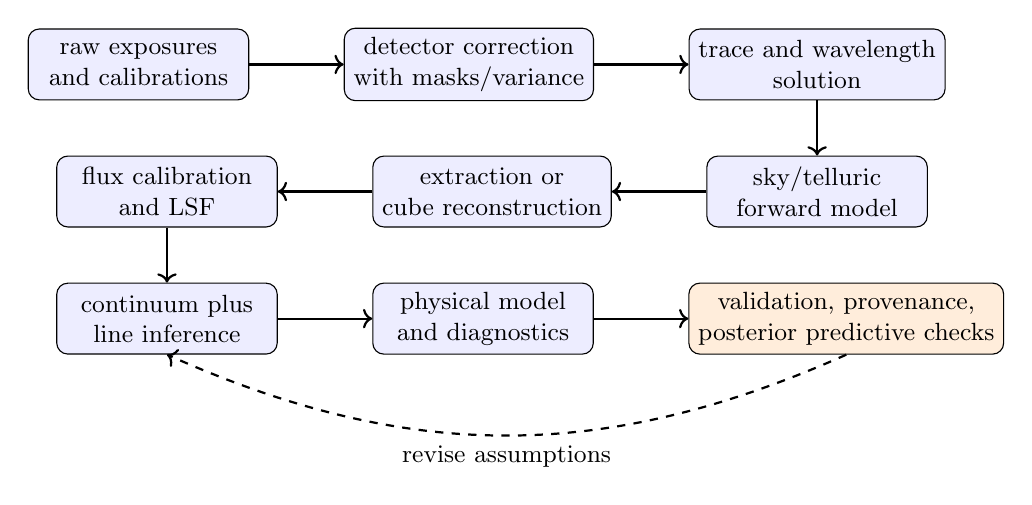
\begin{tikzpicture}[
 node distance=7mm and 12mm,
 every node/.style={font=\small},
 box/.style={draw,rounded corners,align=center,minimum width=28mm,
 minimum height=9mm,fill=blue!7},
 warn/.style={draw,rounded corners,align=center,minimum width=28mm,
 minimum height=9mm,fill=orange!14},
 arrow/.style={->,thick}
]
 \node[box] (raw) {raw exposures\\and calibrations};
 \node[box,right=of raw] (det) {detector correction\\with masks/variance};
 \node[box,right=of det] (map) {trace and wavelength\\solution};
 \node[box,below=of map] (bg) {sky/telluric\\forward model};
 \node[box,left=of bg] (ext) {extraction or\\cube reconstruction};
 \node[box,left=of ext] (flux) {flux calibration\\and LSF};
 \node[box,below=of flux] (fit) {continuum plus\\line inference};
 \node[box,right=of fit] (phys) {physical model\\and diagnostics};
 \node[warn,right=of phys] (audit) {validation, provenance,\\posterior predictive checks};
 \draw[arrow] (raw)--(det); \draw[arrow] (det)--(map);
 \draw[arrow] (map)--(bg); \draw[arrow] (bg)--(ext);
 \draw[arrow] (ext)--(flux); \draw[arrow] (flux)--(fit);
 \draw[arrow] (fit)--(phys); \draw[arrow] (phys)--(audit);
 \draw[arrow,dashed] (audit.south) to[bend left=24]
   node[midway,below] {revise assumptions} (fit.south);
\end{tikzpicture}
\caption{Original reduction-to-inference graph.  Masks, variance or covariance, LSF,
and provenance flow with the spectrum.  Validation is a feedback loop rather than a
final cosmetic step.}
\label{fig:analysis-graph}
\end{figure}

Figure~\ref{fig:analysis-graph} emphasizes that every product should retain auxiliary
information: data-quality masks, propagated uncertainty, wavelength and spatial
coordinates, spectral resolution, exposure metadata, and links to calibration
versions.  A flux array without these is not analysis-ready.

\section{Continuum modeling}

Line measurements are conditional on a continuum model.  Possible components include
stellar populations and absorption, a nonthermal power law, nebular continuum, dust
emission, Fe complexes, scattered light, and residual response structure.  Local
polynomials are effective over narrow intervals but can absorb broad wings.  Physical
templates extrapolate more meaningfully but carry population and abundance mismatch.

The continuum and line should be fitted jointly whenever their uncertainties are
coupled.  Subtracting a best-fit continuum and then treating it as exact understates
line-flux uncertainty.  For Balmer emission, underlying stellar absorption can be
comparable to the nebular equivalent width, especially in weakly star-forming regions.
A flexible stellar-continuum model is then not optional.

Continuum placement can be stress-tested by changing windows, polynomial order, or
template library and examining the shift in line parameters.  These shifts are a
model-systematic term, not a reason to select whichever configuration yields the
smallest formal error.

\section{Forward line-profile fitting}

A common model for a local spectral interval is
\begin{equation}
 m(\lambda)=C(\lambda;\boldsymbol{c})+
 \left[\sum_{k=1}^{K}F_k\,
 p_k(\lambda;v_k,\sigma_k)\right]*L(\lambda),
 \label{eq:spectral-forward-model}
\end{equation}
sampled and integrated over the same pixels as the data.  Here each $p_k$ is normalized
to unit area, so $F_k$ is integrated flux.  Multiple transitions may share velocity
and dispersion; branching ratios may be fixed only when atomic physics, opacity, and
blending justify doing so.

With residual vector $\boldsymbol{r}=\boldsymbol{d}-\boldsymbol{m}$ and covariance
$\boldsymbol{C}$, the Gaussian log likelihood is
\begin{equation}
 -2\ln\mathcal{L}=
 \boldsymbol{r}^{\mathsf T}\boldsymbol{C}^{-1}\boldsymbol{r}
 +\ln|\boldsymbol{C}|+\mathrm{constant}.
 \label{eq:gaussian-correlated-likelihood}
\end{equation}
Ignoring off-diagonal covariance after resampling can underestimate uncertainties and
make broad low-amplitude residuals appear significant.  When the full covariance is
too costly, an empirical correction from blank-sky apertures or block bootstrap is
better than pretending pixels are independent.

For a Gaussian line in wavelength,
\begin{equation}
 p(\lambda)=\frac{1}{\sqrt{2\pi}\sigma_\lambda}
 \exp\!\left[-\frac{(\lambda-\lambda_c)^2}{2\sigma_\lambda^2}\right],
 \quad
 \mathrm{FWHM}=2\sqrt{2\ln2}\,\sigma_\lambda.
 \label{eq:gaussian-line-model}
\end{equation}
If both source and LSF are Gaussian,
$\sigma_{\rm obs}^2=\sigma_{\rm int}^2+\sigma_{\rm inst}^2$.  Subtraction in
quadrature is invalid for non-Gaussian LSFs, unresolved lines near the boundary
$\sigma_{\rm int}=0$, or blends.  Forward convolution handles these cases more
honestly.

\subsection{Model complexity and components}

Adding Gaussian components will almost always improve least-squares residuals.  A
component should be retained because it is reproducible, physically interpretable,
or required by predictive checks, not merely because an optimizer found it.  Compare
models using held-out pixels, information criteria with their assumptions stated, or
Bayesian evidence when priors are defensible.  Inspect whether inferred components
persist across independent transitions and spatial bins.

Parameters become non-identifiable when components are closer than the resolution or
one has low contrast.  In that regime, the data may constrain total flux and centroid
but not the individual widths and velocities.  Publishing a covariance or posterior
sample makes this distinction visible.

\section{Non-parametric profile measurements}

Non-parametric velocities can summarize asymmetric profiles without assigning each
feature to a Gaussian.  From the continuum-subtracted cumulative flux
\begin{equation}
 \mathcal{F}(v)=\frac{\int_{v_{\min}}^v F(v')\,\mathrm{d}v'}
 {\int_{v_{\min}}^{v_{\max}}F(v')\,\mathrm{d}v'},
 \label{eq:cumulative-line-flux}
\end{equation}
define $v_p$ by $\mathcal{F}(v_p)=p/100$.  Measures such as
$W_{80}=v_{90}-v_{10}$ and $v_{50}$ are common.  They depend on the integration
window, continuum, noise, and LSF.  Negative pixels and absorption complicate the
cumulative distribution, so the exact algorithm must be documented.

The flux-weighted centroid and second moment are
\begin{equation}
 \bar v=\frac{\int vF(v)\,\mathrm{d}v}{\int F(v)\,\mathrm{d}v},
 \qquad
 \sigma_v^2=\frac{\int(v-\bar v)^2F(v)\,\mathrm{d}v}{\int F(v)\,\mathrm{d}v}.
 \label{eq:line-moments}
\end{equation}
Moments are sensitive to weak wings and window choices.  Monte Carlo propagation
should perturb the continuum and correlated noise, not only individual flux pixels.

\section{Equivalent width, flux, and luminosity}

Rest-frame equivalent width separates a line from the local continuum scale.  For
emission, some communities use positive and others negative signs; the convention
must be explicit.  The line flux from a fitted profile is preferable to summing a
fixed window when blends or masked pixels matter.  Direct integration remains a
valuable model check.

Uncertainty in integrated flux for weights $w_i$ is
\begin{equation}
 \mathrm{Var}(F)=\boldsymbol{w}^{\mathsf T}
 \boldsymbol{C}\boldsymbol{w},
 \label{eq:integrated-flux-covariance}
\end{equation}
not merely $\sum_i w_i^2\sigma_i^2$ unless the covariance is diagonal.  Luminosity
then requires a cosmology and luminosity distance.  For gravitationally lensed
sources, quote whether luminosity is apparent or corrected by a magnification model.

\section{Detection significance and upper limits}

A line ``detected at $5\sigma$'' is incomplete unless the search procedure is stated.
If wavelength and width were scanned over many possibilities, the false-alarm rate
is larger than the single-trial Gaussian tail.  A matched-filter amplitude for a
known template $\boldsymbol{p}$ is
\begin{equation}
 \widehat{A}=\frac{\boldsymbol{p}^{\mathsf T}
 \boldsymbol{C}^{-1}\boldsymbol{d}}
 {\boldsymbol{p}^{\mathsf T}\boldsymbol{C}^{-1}\boldsymbol{p}},
 \qquad
 \sigma_A^2=\left(\boldsymbol{p}^{\mathsf T}
 \boldsymbol{C}^{-1}\boldsymbol{p}\right)^{-1}.
 \label{eq:matched-filter}
\end{equation}
The template includes the assumed intrinsic width and LSF.  Searching a template bank
requires calibrating the maximum statistic using blank spectra, permutations, or
simulations that reproduce the entire reduction.

An upper limit is conditional on line width, centroid window, profile, and confidence
construction.  For a nondetection of an unresolved line, a statement such as
``$3\sigma$ flux limit for a Gaussian with FWHM
$100\,\mathrm{km\,s^{-1}}$ at the systemic redshift'' is reusable.  A bare number is
not.  Negative fitted fluxes should generally remain in ensemble analyses; clipping
them to zero biases stacked and population estimates.

\subsection{Worked example: width-dependent flux limit}

Assume independent spectral samples of width $\delta v=20\,\mathrm{km\,s^{-1}}$
with flux-density uncertainty $s$.  A top-hat line of width
$\Delta v=100\,\mathrm{km\,s^{-1}}$ spans $N=5$ samples, so the integrated-noise
scale is $s\,\delta v\sqrt{N}$.  If instead one assumes
$\Delta v=400\,\mathrm{km\,s^{-1}}$, $N=20$ and the flux limit doubles.  Correlated
noise changes the square-root scaling.  This is why line-width assumptions belong in
upper-limit tables.

\section{Integral-field spectroscopy}

An integral-field unit samples two spatial dimensions and one spectral dimension, but
the reconstructed cube has a three-dimensional response: a spatial point-spread
function (PSF), spectral LSF, pixel footprint, and covariance.  Resampling detector
pixels into spaxels correlates both neighboring wavelengths and neighboring spatial
samples.

Common spatial binning methods target a continuum signal-to-noise, yet emission-line
signal-to-noise may follow a different morphology.  Binning based on the line being
tested can also introduce selection bias.  A defensible strategy defines bins using
an independent quantity, fits all spaxels hierarchically, or demonstrates through
injection tests that adaptive selection does not fabricate gradients.

Beam smearing mixes velocities within the PSF and can mimic high dispersion where a
velocity gradient is steep.  The observed cube should be compared to a source model
convolved spatially and spectrally.  Subtracting a scalar instrumental width from each
spaxel cannot correct spatial beam smearing.

\section{Validation by injection and repetition}

End-to-end injection tests place synthetic sources into raw or minimally processed
data, run the normal pipeline, and compare recovered parameters with truth.  They can
measure completeness, flux bias, centroid bias near sky lines, component
recoverability, and the effect of covariance.  Injections should span morphology,
line width, equivalent width, and background conditions rather than a single ideal
case.

Other high-value checks include:
\begin{itemize}
 \item fitting independent exposures and detector subsets separately;
 \item comparing integrated flux with direct aperture sums;
 \item verifying fixed atomic branching ratios where opacity is negligible;
 \item checking skylines or calibration lamps for LSF and wavelength residuals;
 \item measuring blank apertures with the same extraction and fitting procedure;
 \item examining posterior predictive residuals in detector and physical coordinates;
 \item repeating measurements under plausible continuum and mask choices.
\end{itemize}

\section{A minimum reproducible line record}

Every published line measurement should be accompanied, directly or in machine-readable
metadata, by:
\begin{enumerate}
 \item transition identifier, rest wavelength, air/vacuum convention, and atomic-data
 source;
 \item observed frame and velocity convention;
 \item aperture, PSF, slit losses, and extraction method;
 \item continuum model, fit window, masks, and blend constraints;
 \item LSF model and spectral sampling;
 \item flux or equivalent width with statistical and systematic uncertainties;
 \item covariance or a documented approximation to it;
 \item attenuation, lensing, and aperture corrections;
 \item nondetection assumptions and search trials;
 \item software version, configuration, calibration version, and provenance links.
\end{enumerate}
This record turns a table of numbers into scientific evidence that another researcher
can audit, combine, or reinterpret.


\part{Gas in and around Galaxies}
% Line Atlas chapter draft.
% Suggested dependencies: amsmath, amssymb, siunitx, booktabs, tabularx,
% threeparttable, tikz, pgfplots, xcolor, hyperref.

\chapter{Line Formation and the Logic of Spectral Diagnostics}
\label{chap:line-formation-diagnostics}
\chaptermark{Line Formation and Diagnostics}

A spectrum contains many transitions but comparatively few independent pieces of
physical information.  Lines from a common ion share an abundance and ionization
fraction; multiplets share upper or lower states; every transition is filtered by the
same foreground dust and the same instrument.  The aim of diagnostic spectroscopy is
therefore not to attach one physical parameter to each line.  It is to identify line
combinations in which unwanted factors cancel and the desired dependence remains.
This chapter develops that logic for recombination lines, collisionally excited
lines, fine-structure transitions, resonance absorption, and molecules.  Standard
references include \citet{OsterbrockFerland2006}, \citet{DopitaSutherland2003},
\citet{Draine2011}, and \citet{Tielens2005}.

\section{Ionization balance is a rate problem}

The ionic abundance of an element is controlled by competing processes rather than
by a single ``formation temperature.''  In photoionized gas, a schematic balance
between stages $X^i$ and $X^{i+1}$ is
\begin{equation}
 n(X^i)\Gamma_i + n_en(X^i)C_i(T)
 =n_en(X^{i+1})\alpha_{i+1}(T)
  + n(X^{i+1})n_{\rm H^0}k_{\rm ce}(T),
 \label{eq:ionization-balance-general}
\end{equation}
where $\Gamma_i$ is a photoionization rate, $C_i$ a collisional ionization
coefficient, $\alpha_{i+1}$ the total radiative plus dielectronic recombination
coefficient, and $k_{\rm ce}$ represents charge exchange.  The photoionization rate
depends on the radiation field throughout the ionizing continuum,
\begin{equation}
 \Gamma_i=4\pi\int_{\nu_i}^{\infty}
 \frac{J_\nu}{h\nu}\sigma_i(\nu)\,\mathrm{d}\nu .
 \label{eq:photoionization-rate}
\end{equation}
An ionization threshold therefore does not specify the characteristic photon energy;
the product $J_\nu\sigma_i/\nu$ weights the actual photons doing the work.

The dimensionless ionization parameter is the number density of hydrogen-ionizing
photons relative to hydrogen atoms,
\begin{equation}
 U\equiv\frac{\Phi_{\rm H}}{n_{\rm H}c}
 =\frac{Q_{\rm H}}{4\pi r^2n_{\rm H}c}
 \label{eq:ionization-parameter}
\end{equation}
for an isotropic source emitting $Q_{\rm H}$ ionizing photons per second at distance
$r$.  A plane-parallel model often uses $U$ at its illuminated face; a spherical
nebula has a distribution of $U$.  Metal-line ratios can constrain $U$ only jointly
with spectral hardness, abundance pattern, pressure, and geometry.

In low-density, collisionally ionized equilibrium (CIE), ionization fractions are
primarily functions of temperature because both ionization and recombination rates
scale with $n_e$.  The familiar temperature at which an ion's CIE fraction peaks is
not a unique temperature of origin.  The same ion may exist in photoionized gas at a
much lower kinetic temperature, in a rapidly cooling nonequilibrium plasma, or at a
conductive or turbulent interface.  Thus O\,VI is evidence for highly ionized oxygen,
not by itself proof of gas at one particular temperature
\citep{GnatSternberg2007,TumlinsonPeeplesWerk2017}.

\subsection{Equilibrium timescales}

Equilibrium is plausible only if microscopic rates are fast compared with changes in
the gas.  A useful recombination timescale is
\begin{equation}
 t_{\rm rec}\simeq\frac{1}{\alpha(T)n_e}.
 \label{eq:recombination-timescale}
\end{equation}
At sufficiently low density, a radiation field or temperature can change faster than
ions recombine.  Cooling gas can then remain overionized relative to CIE, while gas
recently exposed to a source can remain underionized.  The diagnostic question is not
whether an equilibrium table exists, but whether $t_{\rm rec}$ and the ionization
timescale are short relative to the cooling, dynamical, and source-variability
timescales.

\section{Hydrogen and helium recombination spectra}

An ionizing photon absorbed by hydrogen creates a photoelectron.  Recombination and
cascade subsequently distribute photons among continua and lines.  In the standard
Case A idealization, every recombination line photon escapes.  In Case B, Lyman-series
photons are assumed optically thick and are converted through repeated absorption and
cascade, while most Balmer and longer-wavelength photons escape.  Neither case is a
universal property of an H\,II region; they are limiting transfer prescriptions
\citep{OsterbrockFerland2006}.

For an ionization-bounded nebula in steady state,
\begin{equation}
 Q_{\rm H,abs}=\int_V n_en_p\alpha_B(T)\,\mathrm{d}V,
 \label{eq:stromgren-balance}
\end{equation}
and a recombination-line luminosity is
\begin{equation}
 L_{ul}=h\nu_{ul}\frac{\alpha^{\rm eff}_{ul}(T)}{\alpha_B(T)}
 Q_{\rm H,abs}.
 \label{eq:recombination-luminosity-qh}
\end{equation}
This relation motivates H$\alpha$ and other recombination lines as star-formation
tracers.  It fails in predictable directions when ionizing photons escape, are
absorbed by dust, arise from an active nucleus or shocks, or when the assumed stellar
population does not represent the actual age and initial mass function
\citep{KennicuttEvans2012}.

\subsection{Balmer decrements and attenuation}

If the intrinsic ratio $R_{\rm int}=F({\rm H}\alpha)/F({\rm H}\beta)$ is known from
recombination theory, a foreground-screen color excess follows from
\begin{equation}
 E(B-V)=\frac{2.5}{k({\rm H}\beta)-k({\rm H}\alpha)}
 \log_{10}\!\left(\frac{R_{\rm obs}}{R_{\rm int}}\right),
 \label{eq:balmer-decrement-ebv}
\end{equation}
where $A_\lambda=k(\lambda)E(B-V)$.  This compact equation hides three model choices:
the intrinsic ratio depends weakly on temperature and density; the attenuation curve
must suit the source; and a mixed dust--emitter geometry is not a foreground screen.
Stellar Balmer absorption, flux-calibration slope, and differential aperture losses
can all bias $R_{\rm obs}$.  Infrared Paschen or Brackett lines extend the wavelength
lever arm and are less extinguished, but cross-instrument calibration can replace one
systematic with another \citep{Fitzpatrick1999}.

\subsection{Worked example: screen attenuation from
H\texorpdfstring{$\alpha$/H$\beta$}{-alpha/H-beta}}

Assume $R_{\rm obs}=4.0$, $R_{\rm int}=2.86$, and an adopted curve with
$k({\rm H}\beta)=3.61$ and $k({\rm H}\alpha)=2.53$.  Then
\begin{equation}
 E(B-V)=\frac{2.5}{1.08}\log_{10}(4.0/2.86)\simeq0.34~\mathrm{mag}.
\end{equation}
The attenuation correction to H$\alpha$ is
$10^{0.4k({\rm H}\alpha)E(B-V)}\simeq2.2$.  Reporting only the corrected luminosity
would conceal the dominant assumptions.  A reproducible measurement should state
the attenuation law, intrinsic decrement, stellar-continuum treatment, and whether
the correction refers to nebular or stellar reddening.

\section{Collisionally excited lines}

Forbidden and semiforbidden lines are not ``unlikely'' in the low-density universe.
Their small spontaneous rates allow metastable levels to radiate because the time
between particle collisions is long.  An excitation from $l$ to $u$ samples the
high-energy tail of the electron distribution through the exponential factor in the
rate coefficient.  A ratio of an auroral line from a high excitation energy to a
nebular line from a lower level can therefore be a sensitive electron thermometer.

For [O\,III], a commonly used conceptual ratio is
\begin{equation}
 R_{\rm OIII}=\frac{I(4959)+I(5007)}{I(4363)}.
 \label{eq:oiii-temperature-ratio}
\end{equation}
At densities below the relevant critical densities, $R_{\rm OIII}$ declines as
temperature rises because excitation of the auroral upper level becomes less
Boltzmann-suppressed.  At higher density, differential collisional de-excitation also
changes the ratio.  A five-level atom calculation, not a single analytic inversion,
is the normal inference tool.

Doublets such as [S\,II] $\lambda\lambda6716,6731$ or [O\,II]
$\lambda\lambda3726,3729$ compare levels close in energy but with different
collisional de-excitation rates.  Their ratios primarily constrain electron density,
but become insensitive at both low- and high-density limits.  Because a real aperture
contains a density distribution, the inferred ``density'' is an emissivity-weighted
effective value.

\begin{table}[tbp]
\centering
\caption{Diagnostic design patterns.  Entries describe the main sensitivity, not an
exclusive interpretation.  Atomic data and valid density ranges must accompany any
numerical calibration.}
\label{tab:diagnostic-design-patterns}
\begin{tabularx}{\textwidth}{@{}
 >{\raggedright\arraybackslash}p{0.22\textwidth}
 >{\raggedright\arraybackslash}p{0.28\textwidth}
 >{\raggedright\arraybackslash}X@{}}
\toprule
Pattern & Desired cancellation & Principal caveats \\
\midrule
Same-upper-level branching ratio & Population, abundance, and often temperature &
Differential extinction, blends, opacity, calibration; useful as an internal check \\
Auroral/nebular ratio of one ion & Ionic abundance and nearly all geometry &
Density dependence, recombination contribution, temperature gradients \\
Fine-structure doublet & Abundance and spectral hardness &
Low/high-density asymptotes, more than one collider \\
Adjacent ion stages of one element & Elemental abundance &
Ionization parameter entangled with spectral shape and geometry \\
Hydrogen recombination ratio & Emission measure and elemental abundance &
Transfer case, dust geometry, stellar absorption \\
Resonance-doublet apparent optical depth & Abundance scale and continuum &
Unresolved saturation, partial covering, scattered light \\
Isotopologue ratio & Much excitation physics if levels are matched &
Optical depth, isotope-selective chemistry, abundance-ratio variations \\
\bottomrule
\end{tabularx}
\end{table}

\section{Abundances: ionic measurements and ionization corrections}

An ionic abundance from an optically thin line ratio can be written schematically as
\begin{equation}
 \frac{n(X^i)}{n({\rm H}^+)}=
 \frac{I_\lambda(X^i)}{I({\rm H}\beta)}
 \frac{\epsilon_{{\rm H}\beta}(T,n_e)}
      {\epsilon_\lambda(X^i;T,n_e)}.
 \label{eq:ionic-abundance}
\end{equation}
The elemental abundance requires an ionization correction factor (ICF),
\begin{equation}
 \frac{X}{\mathrm{H}}=\mathrm{ICF}(X)
 \sum_{i\in\mathrm{observed}}\frac{X^i}{\mathrm{H}^+}.
 \label{eq:ionization-correction-factor}
\end{equation}
An ICF is a model statement about unobserved ions, not an observational constant.
It depends on the ionizing spectrum, geometry, and sometimes depletion into dust.

``Direct'' electron-temperature abundances are direct only in the limited sense that
a temperature-sensitive line is measured.  If temperature fluctuates spatially, the
auroral line weights hotter zones disproportionately because of its exponential
emissivity.  Recombination lines respond more weakly to temperature but are faint.
Strong-line metallicity calibrations trade weak-line sensitivity for dependence on a
model or empirical training set.  Different calibrations may differ systematically;
the calibration name and abundance scale are part of the result, not metadata that
can be omitted \citep{KewleyEllison2008,KewleyNichollsSutherland2019}.

\subsection{Ionization-source diagrams}

The Baldwin--Phillips--Terlevich family of diagrams compares a high-excitation line to
a Balmer line and a low-ionization line to another Balmer line
\citep{BaldwinPhillipsTerlevich1981}.  The closeness in wavelength of each ratio
reduces sensitivity to reddening and flux-calibration slope.  Star-forming sequences,
AGN, and shocks occupy different regions because their ionizing spectra and partially
ionized zones differ \citep{KewleyEtAl2001,KauffmannEtAl2003}.

Classification boundaries are not laws of nature.  Integrated spectra can mix H\,II
regions, diffuse ionized gas, shocks, and an AGN.  High-redshift abundance patterns,
pressures, and stellar spectra may shift the star-forming locus.  Spatially resolved
data are particularly vulnerable to low equivalent-width diffuse emission and to
point-spread-function mixing.  Diagnostic diagrams should be treated as projections
of a continuous mixture problem.

\begin{figure}[tbp]
\centering
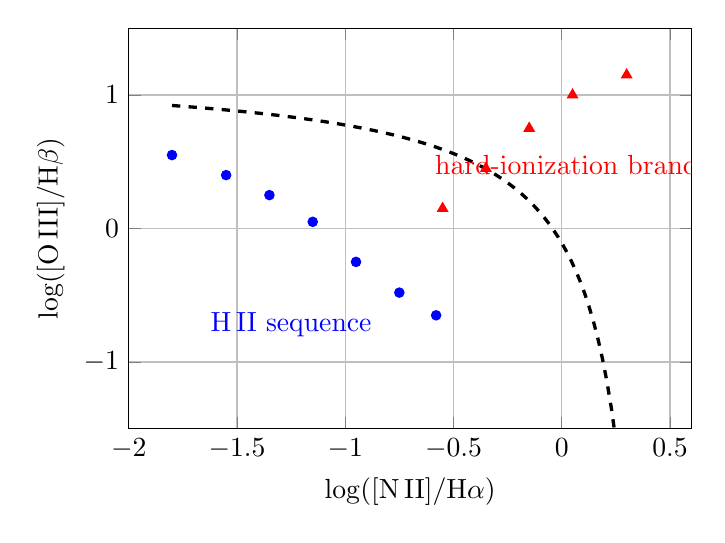
\begin{tikzpicture}
\begin{axis}[
 width=0.72\linewidth,height=0.55\linewidth,
 xlabel={$\log([\mathrm{N\,II}]/\mathrm{H}\alpha)$},
 ylabel={$\log([\mathrm{O\,III}]/\mathrm{H}\beta)$},
 xmin=-2.0,xmax=0.6,ymin=-1.5,ymax=1.5,
 grid=major,
]
 \addplot[only marks,mark=*,mark size=1.7pt,blue]
 coordinates {(-1.8,0.55) (-1.55,0.40) (-1.35,0.25) (-1.15,0.05)
 (-0.95,-0.25) (-0.75,-0.48) (-0.58,-0.65)};
 \addplot[only marks,mark=triangle*,mark size=2.1pt,red]
 coordinates {(-0.55,0.15) (-0.35,0.45) (-0.15,0.75) (0.05,1.0)
 (0.30,1.15)};
 \addplot[very thick,dashed,domain=-1.8:0.25,samples=100]
 {0.61/(x-0.47)+1.19};
 \node[blue] at (axis cs:-1.25,-0.72) {H\,II sequence};
 \node[red] at (axis cs:0.05,0.48) {hard-ionization branch};
\end{axis}
\end{tikzpicture}
\caption{Original PGFPlots concept for an emission-line diagnostic plane.  The
points are synthetic and the dashed curve is illustrative; the production caption
must identify any adopted empirical or theoretical boundary and its domain of
validity.}
\label{fig:diagnostic-plane-concept}
\end{figure}

\section{Fine-structure lines and infrared diagnostics}

Fine-structure transitions connect closely spaced levels within a ground electronic
term.  Their excitation energies correspond to tens to thousands of kelvin, making
them bright coolants of gas too cool to radiate optical collisionally excited lines.
Important examples include [C\,II] $158\,\mu$m, [O\,I] $63$ and $145\,\mu$m,
[O\,III] $52$ and $88\,\mu$m, [N\,II] $122$ and $205\,\mu$m, and [Ne\,II]
$12.8\,\mu$m.  Dust extinction is greatly reduced in the infrared, though dust
continuum opacity may still matter in compact, high-column sources.

Several colliders can excite the same line.  For [C\,II], electrons, H, and
H$_2$ have different rate coefficients and dominate in different phases.  An
observed [C\,II] luminosity can combine ionized gas, atomic photodissociation layers,
and CO-faint molecular envelopes.  [N\,II], which requires ionized gas, can help
estimate the ionized contribution if abundance and density are constrained.  A line
frequently used as a star-formation proxy is therefore not emitted by a single
``star-forming phase.''

The luminosity of a two-level fine-structure line per ion approaches a maximum in the
thermalized, optically thin limit.  Consequently line luminosity gives a strict
minimum mass of the emitting ion only after adopting temperature, collider density,
and upper-level fraction.  Optical depth and subcritical excitation increase the
required mass.

\section{Molecular rotational and vibrational lines}

For a linear rigid rotor with rotational constant $B$, idealized level energies are
\begin{equation}
 E_J=hBJ(J+1),\qquad g_J=2J+1,
 \label{eq:rigid-rotor}
\end{equation}
and allowed electric-dipole rotational transitions have $\Delta J=\pm1$ when the
molecule has a permanent dipole moment.  CO has low-lying transitions that are easy
to excite in cold molecular gas.  H$_2$ has no permanent dipole; its quadrupole
rotational lines require warmer material, so cold H$_2$ is usually inferred through
CO, dust, gamma rays, or absorption rather than direct emission.

If lines are optically thin, share one excitation temperature, and beam filling is
known, a rotational diagram uses
\begin{equation}
 \ln\!\left(\frac{N_u}{g_u}\right)
 =\ln\!\left(\frac{N_{\rm tot}}{Q(T_{\rm ex})}\right)
 -\frac{E_u}{kT_{\rm ex}}.
 \label{eq:rotational-diagram}
\end{equation}
The inverse slope is $-T_{\rm ex}$ and the intercept encodes total column through the
partition function $Q$.  Curvature can indicate multiple temperatures, non-LTE
populations, opacity, or inconsistent emitting areas.  A straight line does not prove
LTE; limited dynamic range can hide departures.

For unresolved sources, brightness-temperature line luminosity is often denoted
$L'$ in units of $\mathrm{K\,km\,s^{-1}\,pc^2}$.  Molecular mass is then
\begin{equation}
 M_{\rm mol}=\alpha_{\rm CO}L'_{\rm CO(1-0)},
 \label{eq:alpha-co}
\end{equation}
where the inclusion of helium must be stated.  The conversion factor varies with
metallicity, shielding, surface density, temperature, and dynamics; a Milky-Way disk
value should not be applied automatically to low-metallicity dwarfs or compact
starbursts \citep{BolattoWolfireLeroy2013}.

\subsection{Worked example: a two-line excitation temperature}

Suppose optically thin measurements yield upper-level columns $N_1$ and $N_2$ for
energies $E_1<E_2$.  Equation~\eqref{eq:rotational-diagram} gives
\begin{equation}
 T_{\rm ex}=\frac{E_2-E_1}{k}
 \left[\ln\!\left(\frac{N_1g_2}{N_2g_1}\right)\right]^{-1}.
 \label{eq:two-line-tex}
\end{equation}
Let $(E_2-E_1)/k=11.1$~K and
$N_1g_2/(N_2g_1)=2.0$.  Then $T_{\rm ex}=16.0$~K.  This is an excitation
temperature between two states, not necessarily the kinetic temperature.  If the
density is subcritical, radiative trapping or the cosmic microwave background can
set $T_{\rm ex}$.  At redshift $z$, the background temperature
$T_{\rm CMB}=2.725(1+z)$~K both excites the molecule and reduces observed contrast.

\section{Absorption-line column densities}

Normalized absorption directly measures apparent optical depth,
\begin{equation}
 \tau_a(v)=\ln\!\left[\frac{F_c(v)}{F(v)}\right],
 \label{eq:apparent-optical-depth}
\end{equation}
and the apparent column-density profile is
\begin{equation}
 N_a(v)=\frac{m_ec}{\pi e^2}
 \frac{\tau_a(v)}{f\lambda_0}.
 \label{eq:aod-column}
\end{equation}
In practical units,
\begin{equation}
 N_a(v)=3.768\times10^{14}
 \frac{\tau_a(v)}{f(\lambda_0/\text{\AA})}
 \quad \mathrm{cm^{-2}\,(km\,s^{-1})^{-1}}.
 \label{eq:aod-practical}
\end{equation}
Integrating over velocity yields an apparent ionic column.  Agreement between
$N_a(v)$ profiles for two transitions of the same ion with different $f\lambda$
supports adequate resolution.  A smaller apparent column in the stronger line flags
unresolved saturation \citep{SavageSembach1991,FoxSavageWakker2005}.

Partial covering changes the residual intensity to
\begin{equation}
 \frac{F(v)}{F_c}=1-C_f(v)+C_f(v)e^{-\tau(v)}.
 \label{eq:partial-covering}
\end{equation}
A saturated line can therefore have a nonzero core.  Scattered light, unrelated
continuum components, and instrumental background can produce the same symptom.
Doublet fitting may constrain $C_f$ and $\tau$, but only within the chosen geometry.

\section{Masers, inversions, and negative opacity}

If $n_u/g_u>n_l/g_l$, the stimulated-emission term exceeds true absorption and
$\alpha_\nu<0$.  Equation~\eqref{eq:homogeneous-slab} then describes exponential
amplification rather than attenuation.  Astrophysical masers require a pump that
creates the inversion, a velocity-coherent path, and a seed radiation field.
Unsaturated maser intensity grows approximately exponentially with path length;
saturation couples the radiation back to the level populations and limits growth.
Narrowness, high brightness temperature, variability, and polarization can reveal
masing, but isotropic luminosity is misleading because the emission may be strongly
beamed.

\section{A diagnostic is a model comparison}

Every line ratio can be written abstractly as a forward model
\begin{equation}
 \boldsymbol{F}_{\rm pred}=
 \mathcal{M}(T,n,\boldsymbol{Z},U,J_\nu,\boldsymbol{v},\mathcal{G},
 \boldsymbol{a}),
 \label{eq:diagnostic-forward-model}
\end{equation}
where $\mathcal{G}$ denotes geometry and $\boldsymbol{a}$ atomic or molecular data.
Inference asks which parameter combinations are consistent with measured fluxes and
their covariance.  A sound atlas therefore records for each diagnostic:
\begin{enumerate}
 \item the transitions and adopted atomic data;
 \item the dominant production and destruction mechanisms;
 \item the density, temperature, abundance, and ionization ranges over which the
 calibration was constructed;
 \item assumptions about equilibrium, opacity, geometry, and radiation field;
 \item known degeneracies and at least one independent cross-check;
 \item whether limits, nondetections, and calibration covariance were included.
\end{enumerate}
The value of a line lies not in a single canonical interpretation, but in knowing
precisely which physical alternatives it can distinguish.

% Line Atlas chapter draft.
% Suggested dependencies: amsmath, amssymb, siunitx, booktabs, tabularx,
% tikz, pgfplots, xcolor, hyperref.

\chapter{The Multiphase Interstellar Medium, PDRs, and Molecular Gas}
\label{chap:ism-pdr-molecular}
\chaptermark{The Multiphase Interstellar Medium}

The interstellar medium (ISM) is a coupled system of gas, dust, magnetic fields,
cosmic rays, and radiation.  Its named ``phases'' are useful landmarks in density and
temperature, not sealed reservoirs.  Material moves among them through cooling,
heating, compression, rarefaction, ionization, recombination, molecule formation,
feedback, and galactic dynamics.  Spectral lines reveal this circulation because each
transition selects a different combination of abundance, excitation, optical depth,
and background.

The discussion here follows the physical framework developed in
\citet{Spitzer1978}, \citet{McKeeOstriker1977}, \citet{Draine2011}, and
\citet{Tielens2005}, with phase and small-scale qualifications discussed by
\citet{Cox2005} and \citet{StanimirovicZweibel2018}.  Photodissociation-region physics
is reviewed by \citet{HollenbachTielens1999}, and molecular conversion factors by
\citet{BolattoWolfireLeroy2013}.

\section{A phase is an equilibrium branch, not merely a temperature bin}

For an ideal gas with total particle density $n_{\rm tot}$,
\begin{equation}
 P_{\rm th}=n_{\rm tot}kT.
 \label{eq:thermal-pressure}
\end{equation}
Observers often quote $P_{\rm th}/k$ in units of
$\mathrm{K\,cm^{-3}}$.  Thermal pressure is only one part of the momentum budget:
\begin{equation}
 P_{\rm tot}=P_{\rm th}+P_{\rm turb}+P_B+P_{\rm cr}+P_{\rm rad},
 \qquad P_B=\frac{B^2}{8\pi}.
 \label{eq:total-ism-pressure}
\end{equation}
These terms need not be locally isotropic or in equipartition.  Magnetic tension, for
example, is not captured by treating $P_B$ as an ordinary scalar pressure.

The thermal energy equation can be written schematically as
\begin{equation}
 \frac{3}{2}n_{\rm tot}k\frac{\mathrm{d}T}{\mathrm{d}t}
 =\Gamma-n_en_{\rm H}\Lambda(T,\boldsymbol{x})
 -P_{\rm th}\boldsymbol{\nabla}\!\cdot\boldsymbol{v}
 +\boldsymbol{\nabla}\!\cdot(\kappa\boldsymbol{\nabla}T),
 \label{eq:thermal-energy-ism}
\end{equation}
where $\Gamma$ includes heating per volume, $\Lambda$ summarizes radiative cooling,
and the final terms represent compression or expansion and conduction.  In diffuse
neutral gas, photoelectrons ejected from small grains and polycyclic aromatic
hydrocarbons often provide important heating.  Cosmic-ray ionization, X-rays,
turbulent dissipation, and chemical heating can dominate in shielded or extreme
environments.  Cooling proceeds through species and transitions whose importance
changes with temperature, ionization, density, metallicity, and optical depth.

Thermal equilibrium satisfies $\Gamma=n_en_{\rm H}\Lambda$.  If heating scales
roughly as $n$ while cooling scales roughly as $n^2$, the equilibrium curve in
pressure-density space can have two stable branches separated by an unstable branch.
This motivates cold and warm neutral media that coexist over a range of pressure
\citep{WolfireEtAl2003}.  Turbulence continuously drives gas away from exact
equilibrium, so observed distributions are broad rather than delta functions.

For isobaric perturbations, the Field criterion may be expressed using the net
cooling per mass or volume with care about convention.  A practical statement is that
an equilibrium is unstable when a small temperature decrease at fixed pressure makes
net cooling stronger, amplifying the perturbation.  Quoting ``thermally unstable''
gas from temperature alone assumes a heating and cooling model.

\begin{figure}[tbp]
\centering
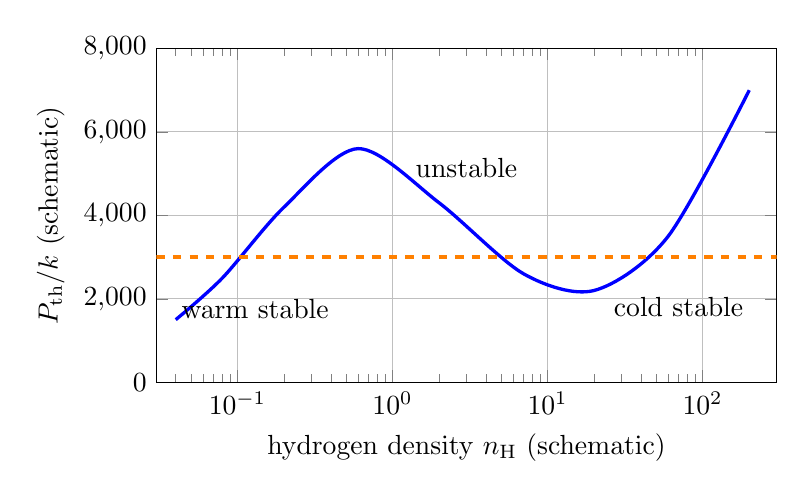
\begin{tikzpicture}
\begin{semilogxaxis}[
 width=0.78\linewidth,height=0.48\linewidth,
 xlabel={hydrogen density $n_{\rm H}$ (schematic)},
 ylabel={$P_{\rm th}/k$ (schematic)},
 xmin=0.03,xmax=300,ymin=0,ymax=8000,
 grid=major,
]
 \addplot[very thick,blue,smooth] coordinates {
 (0.04,1500) (0.08,2500) (0.2,4200) (0.6,5600)
 (2.0,4300) (7.0,2600) (20,2200) (60,3500) (200,7000)};
 \addplot[very thick,dashed,orange] coordinates {(0.03,3000) (300,3000)};
 \node at (axis cs:0.13,1750) {warm stable};
 \node at (axis cs:3.0,5150) {unstable};
 \node at (axis cs:70,1800) {cold stable};
\end{semilogxaxis}
\end{tikzpicture}
\caption{Original schematic of a two-phase thermal-equilibrium curve.  The shape is
pedagogical rather than a numerical cooling calculation.  A horizontal pressure can
intersect warm and cold stable branches, with an intermediate unstable solution.
Radiation field, metallicity, dust, cosmic rays, and shielding shift the curve.}
\label{fig:two-phase-schematic}
\end{figure}

\section{Working inventory of ISM regimes}

Table~\ref{tab:ism-regime-inventory} gives orientation values.  They are deliberately
shown as broad ranges; a phase label should never replace a measured density or
temperature.

\begin{table}[tbp]
\centering
\caption{Orientation map for interstellar regimes.  Values vary with galactic
environment and are not classification boundaries.}
\label{tab:ism-regime-inventory}
\begin{tabularx}{\textwidth}{@{}
 >{\raggedright\arraybackslash}p{0.18\textwidth}
 >{\raggedright\arraybackslash}p{0.15\textwidth}
 >{\raggedright\arraybackslash}p{0.16\textwidth}
 >{\raggedright\arraybackslash}X@{}}
\toprule
Regime & Typical $T$ & Indicative $n_{\rm H}$ & Representative probes \\
\midrule
Cold neutral medium & tens to a few hundred K &
$\sim1$--$10^2\,\mathrm{cm^{-3}}$ & H\,I 21-cm absorption/emission,
C\,I fine structure, [C\,II], Na\,I, K\,I \\
Warm neutral medium & several $10^3$--$10^4$ K &
$\sim0.1$--$1\,\mathrm{cm^{-3}}$ & H\,I 21 cm, UV low-ion absorption,
broad H\,I absorption \\
Warm ionized medium & roughly $10^4$ K &
$\sim10^{-2}$--$1\,\mathrm{cm^{-3}}$ & H$\alpha$, radio free--free,
pulsar dispersion, [N\,II], [S\,II] \\
Classical H\,II region & roughly $10^4$ K &
$\sim10$--$10^4\,\mathrm{cm^{-3}}$ & H and He recombination lines,
[O\,II], [O\,III], [N\,II], [S\,II] \\
Hot ionized medium & $10^5$--$10^7$ K &
$\sim10^{-4}$--$10^{-2}\,\mathrm{cm^{-3}}$ & soft X-ray lines and
continuum, O\,VI at interfaces, highly ionized absorption \\
Diffuse molecular gas & $\sim20$--$100$ K &
$\sim10^2$--$10^3\,\mathrm{cm^{-3}}$ & CO, CH, OH, HCO$^+$ absorption,
dust, gamma rays \\
Dense molecular structures & $\sim10$--$100$ K &
$\gtrsim10^4\,\mathrm{cm^{-3}}$ & NH$_3$, N$_2$H$^+$, HCN, HCO$^+$,
CS, dust continuum \\
\bottomrule
\end{tabularx}
\end{table}

The hot phase has large volume filling potential but small mass density; molecular
structures carry substantial mass in a small volume.  Filling factors are scale and
environment dependent.  A pencil-beam absorption spectrum samples column-weighted
material, while diffuse emission weights emissivity and telescope beam.  Apparent
disagreement can therefore reflect different selection functions rather than
inconsistent physics.

\subsection{Neutral atomic gas and the 21-cm line}

The H\,I hyperfine transition at 1420.4058~MHz connects the triplet and singlet
ground-state configurations.  Its excitation is described by a spin temperature
$T_s$.  For a homogeneous layer in the Rayleigh--Jeans limit,
\begin{equation}
 T_B(v)=T_{\rm bg}e^{-\tau(v)}+T_s\left[1-e^{-\tau(v)}\right].
 \label{eq:hi-transfer}
\end{equation}
Against a bright continuum source, absorption constrains $\tau(v)$; emission and
absorption together constrain $T_s$.  In the optically thin limit,
\begin{equation}
 N_{\rm HI}=1.823\times10^{18}
 \int T_B(v)\,\mathrm{d}v
 \quad\mathrm{cm^{-2}},
 \label{eq:hi-thin-column}
\end{equation}
with $T_B$ in kelvin and $v$ in $\mathrm{km\,s^{-1}}$.  Cold opaque components cause
the optically thin estimate to miss column.  Beam mismatch between emission and
pencil-beam absorption adds another systematic.

Thermal H\,I width sets an upper limit on temperature because turbulence also
broadens the profile.  Decomposing emission into Gaussians does not uniquely assign
physical clouds; regularization and component-count assumptions can dominate the
phase fractions.

\subsection{Warm ionized and hot gas}

Diffuse warm ionized gas is traced by recombination emission, free--free emission,
Faraday rotation, and pulsar dispersion measure
\begin{equation}
 {\rm DM}=\int n_e\,\mathrm{d}\ell.
 \label{eq:dispersion-measure}
\end{equation}
Combining DM with an emission measure $\int n_e^2\mathrm{d}\ell$ can constrain a
characteristic density and filling factor, provided the paths match.  Elevated
low-ionization line ratios in diffuse gas reflect its ionization and heating state and
can contaminate classifications based on integrated galaxy spectra.

Hot gas emits bremsstrahlung and metal lines in the extreme ultraviolet and X-ray.
Its inferred density depends on an emission measure and volume, hence on geometry and
filling factor.  Soft X-ray absorption by foreground gas complicates the coolest hot
components.  Intermediate-temperature ions at interfaces may be far from ionization
equilibrium, making single-temperature CIE fits an approximation.

\section{Photodissociation regions}

A photodissociation region (PDR) is predominantly neutral gas whose heating and
chemistry are controlled substantially by far-ultraviolet photons below the hydrogen
ionization edge.  PDRs occur on molecular-cloud surfaces, within clumpy clouds, around
H\,II regions, in diffuse atomic gas, and on galaxy-wide scales
\citep{HollenbachTielens1999}.  The term describes a regulatory regime, not a simple
geometric shell.

Two useful control parameters are gas density and incident far-UV field.  The latter
is often normalized as $G_0$ to a conventional interstellar band-integrated field, or
as $\chi$ under a different normalization.  These conventions differ; the unit and
reference field must be stated.  Ratios such as $G_0/n_{\rm H}$ influence grain
charging, photoelectric heating efficiency, and the location of chemical transitions.

\begin{figure}[tbp]
\centering
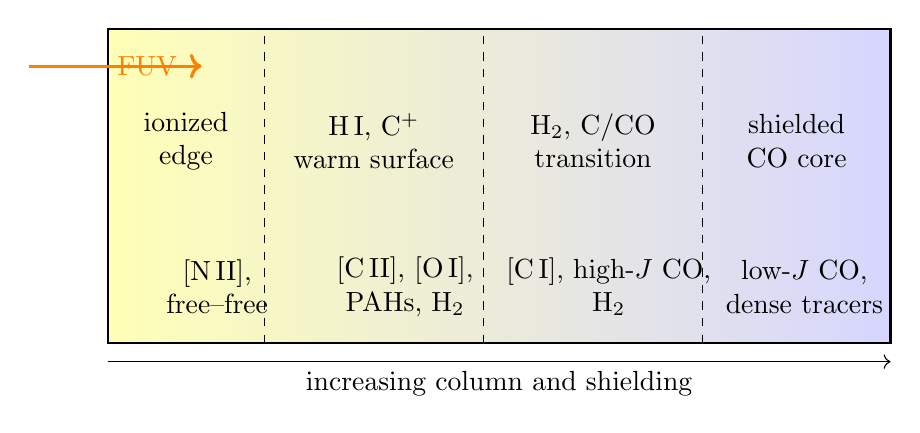
\begin{tikzpicture}[x=0.82\linewidth,y=0.95cm]
 \shade[left color=yellow!28,right color=blue!16] (0,0) rectangle (1,4.2);
 \draw[thick] (0,0) rectangle (1,4.2);
 \draw[->,very thick,orange] (-0.10,3.7)--(0.12,3.7)
   node[left=5pt] {FUV};
 \draw[dashed] (0.20,0)--(0.20,4.2);
 \draw[dashed] (0.48,0)--(0.48,4.2);
 \draw[dashed] (0.76,0)--(0.76,4.2);
 \node[align=center] at (0.10,2.7) {ionized\\edge};
 \node[align=center] at (0.34,2.7) {H\,I, C$^+$\\warm surface};
 \node[align=center] at (0.62,2.7) {H$_2$, C/CO\\transition};
 \node[align=center] at (0.88,2.7) {shielded\\CO core};
 \node[align=center] at (0.14,0.75) {[N\,II],\\free--free};
 \node[align=center] at (0.38,0.75) {[C\,II], [O\,I],\\PAHs, H$_2$};
 \node[align=center] at (0.64,0.75) {[C\,I], high-$J$ CO,\\H$_2$};
 \node[align=center] at (0.89,0.75) {low-$J$ CO,\\dense tracers};
 \draw[->] (0,-0.25)--(1,-0.25)
   node[midway,below] {increasing column and shielding};
\end{tikzpicture}
\caption{Original plane-parallel PDR concept.  Real clouds are porous and illuminated
from multiple directions, so zones overlap in projection.  Transition depths depend
on density, metallicity, dust, radiation spectrum, cosmic rays, and dynamics.}
\label{fig:pdr-layering}
\end{figure}

\subsection{Hydrogen formation and shielding}

In ordinary dusty gas, H$_2$ forms efficiently on grain surfaces.  A schematic
formation rate per volume is
\begin{equation}
 \mathcal{R}_{\rm form}=R_{\rm d}\,n_{\rm H}\,n({\rm H}),
 \label{eq:h2-formation}
\end{equation}
where $R_{\rm d}$ depends on grain abundance, temperature, and sticking physics.  The
unshielded photodissociation rate is reduced by dust attenuation and H$_2$
self-shielding:
\begin{equation}
 \mathcal{R}_{\rm diss}=D_0G_0\,
 f_{\rm sh}(N_{\rm H_2})e^{-\sigma_{d}N_{\rm H}}
 n({\rm H_2}).
 \label{eq:h2-dissociation}
\end{equation}
The H/H$_2$ transition occurs where formation balances the attenuated destruction.
H$_2$ can self-shield through its line spectrum at columns where CO remains
photodissociated.  This produces ``CO-faint'' or ``CO-dark'' molecular gas, especially
at low metallicity where dust shielding per hydrogen nucleus is smaller.

\subsection{Worked example: an \texorpdfstring{H$_2$}{H2} formation time}

Adopt $R_d=3\times10^{-17}\,\mathrm{cm^3\,s^{-1}}$ as an illustrative Milky-Way
value and $n_{\rm H}=100\,\mathrm{cm^{-3}}$.  The characteristic formation time from
mostly atomic gas is
\begin{equation}
 t_{\rm form}\sim(R_dn_{\rm H})^{-1}
 \simeq1.1\times10^7~\mathrm{yr}.
 \label{eq:h2-formation-time-example}
\end{equation}
At ten times higher density the time is roughly ten times shorter, absent changes in
grain properties.  Comparing this time with a turbulent crossing or cloud assembly
time tests chemical equilibrium.  The calculation does not locate the H/H$_2$
front, because photodissociation and shielding were omitted.

\subsection{Carbon chemistry and principal coolants}

At an illuminated surface, carbon is often C$^+$ while hydrogen may already be
neutral.  Increasing shielding permits neutral carbon and eventually CO to become
abundant.  This cartoon is chemically useful but not a strict series of planar
layers: turbulent mixing, cosmic rays, clumping, and nonequilibrium reactions can
place C$^+$, C, and CO together.

[C\,II] $158\,\mu$m and [O\,I] $63\,\mu$m are major coolants over portions of PDR
parameter space.  Their intensities relative to far-infrared dust emission and to one
another are commonly compared with PDR grids to infer density and radiation field.
Degeneracies are common, [C\,II] has ionized-gas contributions, [O\,I] can be optically
thick and self-absorbed, and multiple cloud faces occur within a beam.  A fitted
``$G_0$'' is therefore an effective model parameter unless geometry is constrained.

The photoelectric heating efficiency falls when grains become more positively
charged because electrons are harder to eject.  This helps explain why line-to-FIR
ratios can decline in intense radiation fields, but high gas density, dust-bounded
ionized regions, line opacity, and continuum optical depth can contribute to observed
``line deficits.''

\section{Molecular clouds are dynamical structures}

Molecular clouds are organized hierarchically into complexes, filaments, clumps,
cores, and velocity-coherent structures.  Boundaries defined by CO intensity,
extinction, or a dendrogram need not select the same mass.  A cloud catalog is the
output of a segmentation algorithm and resolution scale as well as an astrophysical
population.

For a structure of mass $M$, effective radius $R$, and one-dimensional velocity
dispersion $\sigma$, the commonly quoted virial parameter is
\begin{equation}
 \alpha_{\rm vir}=\frac{5\sigma^2R}{GM}
 \label{eq:virial-parameter}
\end{equation}
for an idealized uniform sphere without surface pressure or magnetic terms.  Values
near two are often associated with a marginally bound object under particular density
profiles.  Treating equation~\eqref{eq:virial-parameter} as an exact binding criterion
ignores geometry, density gradients, external pressure, magnetic support, mass
uncertainty, and time dependence \citep{McKeeOstriker2007}.

The turbulent Mach number is
\begin{equation}
 \mathcal{M}=\frac{\sigma_{\rm 3D}}{c_s},
 \qquad c_s=\sqrt{\frac{kT}{\mu m_{\rm H}}}.
 \label{eq:mach-number}
\end{equation}
Molecular gas is commonly supersonic on cloud scales.  Shocks create density
structure and dissipate energy; turbulence can both support a region globally and
compress subregions locally.  Line width includes opacity broadening, multiple
components, systematic gradients, and unresolved feedback in addition to turbulence.

\subsection{CO as a mass tracer}

For the CO $J=1\rightarrow0$ line,
\begin{equation}
 N({\rm H_2})=X_{\rm CO}W_{\rm CO},
 \qquad
 M_{\rm mol}=\alpha_{\rm CO}L'_{\rm CO}.
 \label{eq:xco-alpha-co}
\end{equation}
$X_{\rm CO}$ is a column conversion and $\alpha_{\rm CO}$ a luminosity-to-mass
conversion.  Authors must state whether helium is included.  CO(1--0) is usually
optically thick in individual clouds, yet integrated intensity can correlate with
mass because velocity structure exposes different surfaces and cloud-scale linewidth
and size correlate with mass.  This emergent calibration is environmental rather than
fundamental \citep{BolattoWolfireLeroy2013}.

At low metallicity, the H$_2$-bearing envelope outside the CO-rich region becomes a
larger fraction of the cloud, increasing $X_{\rm CO}$.  In warm, high-dispersion
galaxy centers or starbursts, CO luminosity per unit mass can rise, lowering
$\alpha_{\rm CO}$.  Dust-based gas masses offer an independent route but require
dust temperature, opacity, dust-to-gas ratio, and subtraction of atomic gas.

\subsection{Worked example: CO luminosity to molecular mass}

Let a galaxy have
$L'_{\rm CO(1-0)}=2.0\times10^9\,
\mathrm{K\,km\,s^{-1}\,pc^2}$.  Adopting
$\alpha_{\rm CO}=4.35\,
M_\odot(\mathrm{K\,km\,s^{-1}\,pc^2})^{-1}$ including helium gives
\begin{equation}
 M_{\rm mol}=8.7\times10^9\,M_\odot.
\end{equation}
If the environment instead justified
$\alpha_{\rm CO}=0.8$ in the same units, the mass would be
$1.6\times10^9\,M_\odot$.  The factor-of-five spread is a model uncertainty, not a
rounding error.  A publication should state the adopted conversion, environmental
rationale, transition ratio if a higher-$J$ line was observed, and helium convention.

\section{Dense-gas tracers and effective excitation}

Molecules with large dipole moments, such as HCN or HCO$^+$, have large spontaneous
rates and correspondingly high optically thin critical densities.  Calling one line
a ``dense-gas tracer'' does not mean it arises only above its tabulated critical
density.  Radiative trapping reduces effective critical density, multilevel cascades
alter populations, infrared pumping can matter, electron collisions can contribute,
and an extended density distribution emits over a broad range.

A more observationally relevant quantity is an effective excitation density: the
density required to produce a specified line brightness for an adopted column,
temperature, and radiation field.  It is model dependent by design.  Comparing
several transitions and isotopologues provides leverage on opacity and excitation.
Even then, abundance variations from freeze-out, photochemistry, shocks, or cosmic
rays may dominate ratios.

NH$_3$ inversion transitions provide a useful thermometer because ratios of
metastable states respond to kinetic temperature under common conditions.  N$_2$H$^+$
often survives where CO freezes onto grains, while CO desorption can destroy it.
SiO can be enhanced when shocks process grains.  These are chemical tendencies, not
one-to-one labels; the local reaction network and timescale determine the result.

\section{Dust, extinction, and continuum mass}

Optically thin thermal dust emission is commonly modeled as
\begin{equation}
 S_{\nu,\rm obs}=\frac{(1+z)\,\kappa_{\nu,\rm rest}
 M_dB_{\nu,\rm rest}(T_d)}{D_L^2},
 \label{eq:dust-mass-flux}
\end{equation}
under one widespread convention for opacity per dust mass.  Factors of $4\pi$ differ
among emissivity definitions, so dimensional consistency with the adopted $\kappa$
is essential.  A single modified blackbody compresses a temperature distribution
into an effective $T_d$; short-wavelength points weight warm dust and can bias mass
low.  At high optical depth, emission approaches $B_\nu(T)$ and no longer scales
linearly with mass.

Extinction measures a pencil-beam column weighted by grain cross section, whereas
emission measures dust luminosity and temperature.  Comparing them tests geometry and
opacity models.  Converting dust mass to total gas mass requires a dust-to-gas ratio
that varies with metallicity and chemical evolution.

\section{Shocks, interfaces, and phase exchange}

A shock converts bulk kinetic energy into heat, compression, magnetic energy, cosmic
rays, and radiation.  For a strong adiabatic shock in a monatomic gas, the immediate
post-shock temperature is approximately
\begin{equation}
 T_s=\frac{3\mu m_{\rm H}}{16k}v_s^2
 \simeq1.4\times10^5\,\mathrm{K}
 \left(\frac{\mu}{0.61}\right)
 \left(\frac{v_s}{100\,\mathrm{km\,s^{-1}}}\right)^2.
 \label{eq:shock-temperature}
\end{equation}
Radiative shocks develop a cooling and recombination zone that emits ions spanning a
large temperature range.  Their line ratios depend on shock speed, preshock density,
magnetic parameter, abundance, precursor radiation, and completeness of the cooling
zone \citep{DopitaSutherland2003}.

Conductive boundaries, turbulent mixing layers, and cloud ablation also populate
intermediate ions.  A sightline through many interfaces can produce substantial
columns without a large volume of gas at the ion's CIE peak temperature.  Kinematic
alignment, multiple ions, and cooling-time arguments are needed to distinguish
interfaces from a volume-filling phase.

\section{Combining tracers without forcing them into one phase}

A robust multiphase analysis uses a generative mixture rather than assigning each
line to exactly one component.  For line $\ell$,
\begin{equation}
 F_\ell=\sum_p F_{\ell,p}(T_p,n_p,Z_p,U_p,N_p,\ldots),
 \label{eq:multiphase-flux-sum}
\end{equation}
where phases $p$ may include ionized gas, atomic PDR surfaces, CO-faint H$_2$, and
shielded molecular gas.  The data constrain only combinations for which sufficiently
distinct tracers exist.  Priors on pressure balance, abundance continuity, or geometry
should be explicit and tested rather than assumed silently.

The following cross-checks are especially valuable:
\begin{itemize}
 \item compare H\,I emission with absorption to test opacity and spin temperature;
 \item use [N\,II] or other ionized-only lines to estimate the ionized contribution
 to [C\,II];
 \item compare CO-based gas with dust-based gas to expose CO-faint material or
 conversion-factor changes;
 \item use isotopologues and multiple $J$ levels to test CO opacity and excitation;
 \item compare density-squared emission with density-linear absorption or dispersion
 measures to constrain clumping;
 \item align velocity components before combining ionic ratios across transitions.
\end{itemize}
The ISM's complexity is not a failure of the phase framework.  It is the central
observable: line combinations map how matter cycles among thermal, chemical, and
dynamical states.

% Line Atlas chapter draft.
% Suggested dependencies: amsmath, amssymb, siunitx, booktabs, tabularx,
% tikz, pgfplots, xcolor, hyperref.

\chapter{Star Formation Across Scales and the Lines That Trace It}
\label{chap:star-formation}
\chaptermark{Star Formation and Its Tracers}

Star formation connects parsec-scale self-gravitating structures to the integrated
light of galaxies.  Spectral lines enter at every stage: molecular transitions map
the reservoir, dense-gas species select compact structures, infall and outflow shape
profiles, recombination lines count ionizing photons, and metal lines diagnose the
H\,II regions around massive stars.  No single transition measures an instantaneous,
scale-independent ``star-formation rate.''  Each tracer averages over a population,
timescale, extinction geometry, and aperture.

This chapter builds a hierarchy from collapse physics to population calibrations.
Broad theoretical and observational syntheses are provided by
\citet{McKeeOstriker2007} and \citet{KennicuttEvans2012}; dense-core physics is
reviewed by \citet{BerginTafalla2007}.

\section{Gravity, pressure, and characteristic scales}

For isothermal gas of density $\rho$ and sound speed $c_s$, the Jeans length and a
commonly used Jeans mass convention are
\begin{equation}
 \lambda_J=c_s\left(\frac{\pi}{G\rho}\right)^{1/2},
 \qquad
 M_J=\frac{\pi^{5/2}}{6}\frac{c_s^3}{G^{3/2}\rho^{1/2}}.
 \label{eq:jeans-scales}
\end{equation}
Perturbations larger than the Jeans length can grow in the idealized infinite,
uniform, nonmagnetic medium.  Real clouds are finite, turbulent, magnetized, and
externally pressured; Jeans quantities remain useful local scales rather than exact
fragmentation predictions.

The free-fall time of a uniform sphere is
\begin{equation}
 t_{\rm ff}=\left(\frac{3\pi}{32G\rho}\right)^{1/2}.
 \label{eq:free-fall-time}
\end{equation}
Star formation is inefficient per mean-density free-fall time.  A common descriptive
parameter is
\begin{equation}
 \epsilon_{\rm ff}=\frac{\dot M_\star t_{\rm ff}}{M_{\rm gas}}.
 \label{eq:epsilon-ff}
\end{equation}
Its inferred value depends on how a cloud boundary, gas mass, density, stellar
population, and averaging time are defined.  A region that is assembling or
dispersing violates the steady-state interpretation of $\dot M_\star$.

Thermal pressure is rarely the dominant cloud-scale support.  A useful effective
one-dimensional dispersion may combine thermal and nonthermal motions,
\begin{equation}
 \sigma_{\rm eff}^2=c_s^2+\sigma_{\rm nt}^2,
 \label{eq:effective-dispersion}
\end{equation}
but calling every nonthermal line width ``support'' is dangerous.  Converging flows,
rotation, collapse, opacity broadening, and unresolved components all contribute.
Support is a statement about the momentum equation and spatial correlations, not
about linewidth alone.

\subsection{Worked example: free-fall time of a dense clump}

Take molecular gas with number density
$n_{\rm H_2}=10^4\,\mathrm{cm^{-3}}$ and mean mass per H$_2$ molecule including helium
$\mu_{\rm H_2}m_{\rm H}\simeq2.8m_{\rm H}$.  Then
$\rho\simeq4.7\times10^{-20}\,\mathrm{g\,cm^{-3}}$ and
\begin{equation}
 t_{\rm ff}\simeq3.1\times10^5~\mathrm{yr}.
\end{equation}
If the clump has $M=10^4M_\odot$ and
$\epsilon_{\rm ff}=0.01$, its time-averaged star-formation rate would be
$\dot M_\star\simeq3.2\times10^{-4}M_\odot\,\mathrm{yr^{-1}}$.  This estimate is
conditional on the mean density and on a steady efficiency; substructure has shorter
local free-fall times.

\section{Magnetic fields and mass-to-flux balance}

Magnetic fields affect compression, angular-momentum transport, anisotropic motion,
and the coupling of protostellar outflows to gas.  A cloud's mass-to-flux ratio is
often compared with a critical value,
\begin{equation}
 \mu_\Phi\equiv\frac{(M/\Phi_B)}{(M/\Phi_B)_{\rm crit}}.
 \label{eq:mass-to-flux}
\end{equation}
Subcritical structures ($\mu_\Phi<1$) cannot collapse across ordered field lines in
ideal magnetohydrodynamics, while supercritical structures can.  The numerical
critical coefficient depends on geometry.  Zeeman splitting measures a line-of-sight
field component in selected gas, dust polarization traces projected orientation with
grain-alignment assumptions, and Faraday rotation weights $n_eB_\parallel$.  Combining
these into a three-dimensional field demands a geometric model.

Nonideal effects---ambipolar diffusion, Ohmic dissipation, and the Hall effect---allow
field and neutral matter to drift on small scales.  Turbulent reconnection and field
topology further complicate a single diffusion-time picture.  Magnetic criticality
should therefore be inferred as a distribution with projection uncertainty, not a
binary label for one projected map.

\section{From clouds to filaments, clumps, and cores}

Cloud structure is scale free over substantial ranges, and names such as clump and
core partly reflect resolution and tracer choice.  A dense continuum peak may contain
several velocity components; a velocity-coherent feature may have little contrast in
column density.  Catalog completeness depends on spatial filtering and segmentation.

Dense cores are often categorized as starless, prestellar, or protostellar.  A
prestellar designation implies gravitational boundedness, which inherits uncertainty
from mass, temperature, radius, linewidth, density profile, magnetic field, and
external pressure.  A source without an infrared counterpart is not automatically
starless: deeply embedded low-luminosity objects can evade a survey.

Chemical differentiation provides an evolutionary clock only after physical
conditions are modeled.  CO freeze-out at cold high density can enhance N$_2$H$^+$
relative to CO; protostellar heating returns volatile species to the gas; shocks
release grain material and enhance molecules such as SiO.  Reaction and adsorption
timescales vary with density, temperature, ionization, and grain surface area.  A
chemical ``age'' is model dependent.

\section{Infall and accretion signatures}

An optically thick line with an excitation temperature rising inward can show a
brighter blue peak than red peak when the envelope is collapsing and a thinner line
defines the systemic velocity.  The foreground redshifted layer preferentially
absorbs red emission.  This classic blue asymmetry is suggestive, not unique:
multiple clouds, rotation, outflow, and spatially varying excitation can mimic it.
Mapping and comparison of optically thick and thin isotopologues are essential.

Mass infall is sometimes estimated as
\begin{equation}
 \dot M_{\rm inf}=4\pi r^2\rho(r)v_{\rm inf}(r).
 \label{eq:mass-infall-rate}
\end{equation}
Every factor is model dependent.  A fitted profile constrains projected velocity
through a radiative-transfer model; it does not directly measure a spherical mass
flux.  Filamentary accretion, disks, and episodic flow can make the spherical estimate
an orientation-level summary only.

Accretion luminosity onto a protostar of mass $M_\star$ and radius $R_\star$ is
approximately
\begin{equation}
 L_{\rm acc}\simeq f_{\rm acc}\frac{GM_\star\dot M_{\rm acc}}{R_\star},
 \label{eq:accretion-luminosity}
\end{equation}
where $f_{\rm acc}$ accounts for energy advected, radiated elsewhere, or carried by
outflows.  Hydrogen lines such as Br$\gamma$ may correlate empirically with accretion
luminosity in calibrated samples, but geometry, extinction, winds, and stellar mass
limit extrapolation.

\section{Protostellar jets and molecular outflows}

Magnetocentrifugal launching extracts angular momentum and produces fast jets or
winds.  Their interaction entrains molecular gas into broad line wings.  CO maps can
estimate outflow mass, momentum, and kinetic energy after corrections for excitation,
opacity, missing low-velocity gas, abundance, spatial filtering, and inclination.
For channel mass $M(v)$ relative to systemic velocity,
\begin{align}
 P_{\rm out}&=\sum_v M(v)|v-v_{\rm sys}|,\\
 E_{\rm out}&=\frac{1}{2}\sum_vM(v)(v-v_{\rm sys})^2.
 \label{eq:outflow-momentum-energy}
\end{align}
Energy is especially sensitive to faint high-velocity wings, while mass is sensitive
to confusion near the cloud velocity.  A dynamical time $t_{\rm dyn}=R_{\rm proj}/
v_{\rm los}$ combines two projection-dependent quantities and is not necessarily the
true age.  Reporting uncorrected observables alongside model-corrected rates helps
future reinterpretation.

Shock-excited H$_2$, [Fe\,II], SiO, and high-$J$ CO trace different zones of an
outflow.  [Fe\,II] can indicate fast, partially ionized shocks and grain processing;
near-infrared H$_2$ lines select warm molecular material; low-$J$ CO carries much of
the cool entrained mass.  Line luminosity alone cannot inventory the outflow without
a temperature distribution.

\section{\texorpdfstring{H\,II}{H II} regions as ionizing-photon calorimeters}

For uniform hydrogen density $n_{\rm H}$ around a source emitting $Q_{\rm H}$ ionizing
photons per second, the ideal Str\"omgren radius is
\begin{equation}
 R_S=\left(\frac{3Q_{\rm H}}{4\pi\alpha_Bn_e n_p}\right)^{1/3}.
 \label{eq:stromgren-radius}
\end{equation}
After rapid ionization, overpressure drives expansion.  An idealized uniform-medium
solution is
\begin{equation}
 R(t)=R_S\left(1+\frac{7c_it}{4R_S}\right)^{4/7},
 \label{eq:hii-spitzer-expansion}
\end{equation}
where $c_i$ is ionized-gas sound speed.  Density gradients, winds, radiation pressure,
leakage, gravity, magnetic fields, and cloud porosity change the evolution.

The observed recombination luminosity counts ionizations absorbed by gas.  If a
fraction $f_{\rm esc}$ escapes and $f_{\rm dust}$ is absorbed by dust before ionizing
hydrogen, then schematically
\begin{equation}
 Q_{\rm H,gas}=(1-f_{\rm esc}-f_{\rm dust})Q_{\rm H,total}.
 \label{eq:ionizing-photon-budget}
\end{equation}
Age and IMF determine $Q_{\rm H,total}$ per unit star-formation rate.  Binary evolution
and stellar rotation can extend hard ionizing emission beyond the lifetime predicted
by a simple single-star population.

\subsection{Worked example: Str\"omgren scale}

For $Q_{\rm H}=10^{49}\,\mathrm{s^{-1}}$, $n_e\simeq n_p=100\,\mathrm{cm^{-3}}$,
and $\alpha_B=2.6\times10^{-13}\,\mathrm{cm^3\,s^{-1}}$,
\begin{equation}
 R_S\simeq3.1~\mathrm{pc}.
\end{equation}
Reducing density by a factor of ten increases $R_S$ by $10^{2/3}\simeq4.6$.
The calculation assumes uniform fully ionized hydrogen and no dust or leakage; a
clumpy nebula with the same mean density need not have the same recombination rate.

\section{Star-formation-rate tracers as temporal filters}

A luminosity-based calibration can be written
\begin{equation}
 \dot M_\star=C_XL_X,
 \label{eq:sfr-calibration-generic}
\end{equation}
but $C_X$ encodes an IMF, metallicity, stellar-evolution model, star-formation history,
dust treatment, and luminosity definition.  More fundamentally, the luminosity is a
convolution of the past star-formation history with a response kernel,
\begin{equation}
 L_X(t)=\int_0^\infty \dot M_\star(t-\tau)\,
 \ell_X(\tau,Z,\mathrm{IMF})\,\mathrm{d}\tau.
 \label{eq:sfr-response-kernel}
\end{equation}
Ionizing-recombination tracers weight the youngest massive stars; ultraviolet
continuum persists longer; supernova-related radio emission is delayed; infrared
emission depends on dust heating and can include older stars.  Differences among
tracers may reveal burstiness rather than calibration failure.

\begin{table}[tbp]
\centering
\caption{Common star-formation tracers and dominant qualifications.  Timescales are
population dependent and should be computed for the adopted stellar model.}
\label{tab:sfr-tracers}
\begin{tabularx}{\textwidth}{@{}
 >{\raggedright\arraybackslash}p{0.19\textwidth}
 >{\raggedright\arraybackslash}p{0.23\textwidth}
 >{\raggedright\arraybackslash}X@{}}
\toprule
Tracer & What supplies the luminosity & Important qualifications \\
\midrule
H recombination lines & Ionizations absorbed by gas & Dust attenuation, stellar
absorption, photon leakage and dust absorption, AGN/shocks, IMF sampling \\
Thermal radio free--free & Ionized gas powered by ionizing photons & Nonthermal
separation, electron temperature, photon leakage; low extinction \\
UV continuum & Photospheres of young and intermediate-age stars & Dust attenuation,
star-formation history, metallicity, older-population contamination \\
Total or monochromatic IR & Dust heated by absorbed radiation & Cirrus from older
stars, unobscured escape, dust temperature and spectral shape, AGN \\
Hybrid H$\alpha$+IR or UV+IR & Direct plus dust-reprocessed components & Aperture
matching and empirical coefficient depend on population and spatial scale \\
Nonthermal radio & Cosmic-ray electrons accelerated after stellar death & Time delay,
escape and cooling, magnetic field, AGN \\
{[C\,II]} and other cooling lines & Gas cooling linked indirectly to FUV heating &
Multiphase origin, metallicity, line deficits, opacity, AGN/shocks \\
\bottomrule
\end{tabularx}
\end{table}

\begin{figure}[tbp]
\centering
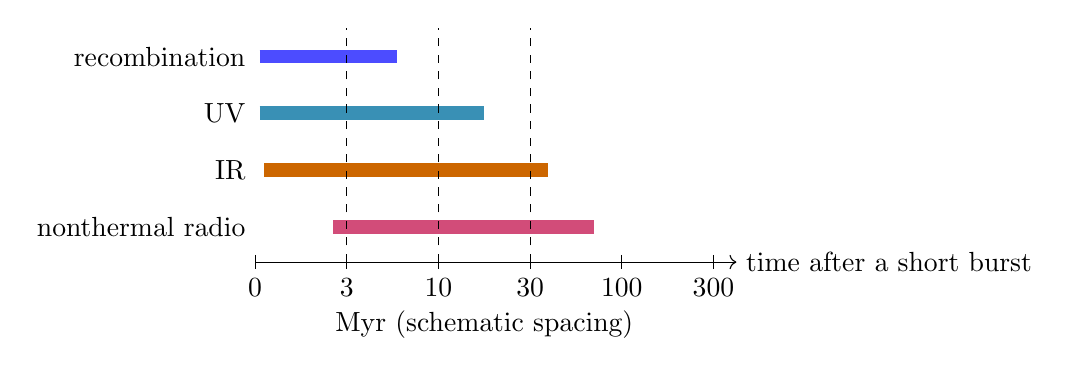
\begin{tikzpicture}[x=0.048\linewidth,y=0.9cm]
 \draw[->] (0,0)--(10.5,0) node[right] {time after a short burst};
 \foreach \x/\lab in {0/0,2/3,4/10,6/30,8/100,10/300}
   {\draw (\x,0.1)--(\x,-0.1) node[below] {\lab};}
 \node[below] at (5,-0.55) {Myr (schematic spacing)};
 \draw[line width=5pt,blue!70] (0.1,2.9)--(3.1,2.9);
 \node[left] at (0,2.9) {recombination};
 \draw[line width=5pt,cyan!70!black] (0.1,2.1)--(5.0,2.1);
 \node[left] at (0,2.1) {UV};
 \draw[line width=5pt,orange!80!black] (0.2,1.3)--(6.4,1.3);
 \node[left] at (0,1.3) {IR};
 \draw[line width=5pt,purple!70] (1.7,0.5)--(7.4,0.5);
 \node[left] at (0,0.5) {nonthermal radio};
 \draw[dashed] (2,0)--(2,3.3); \draw[dashed] (4,0)--(4,3.3);
 \draw[dashed] (6,0)--(6,3.3);
\end{tikzpicture}
\caption{Original qualitative response-window concept.  Bars indicate relative
sensitivity after a short stellar burst, not universal top-hat lifetimes.  Actual
kernels depend on metallicity, IMF, binaries, dust, and observing band.}
\label{fig:sfr-response-windows}
\end{figure}

\subsection{Stochastic populations and small apertures}

Standard calibrations assume that the stellar IMF and evolutionary phases are
adequately sampled.  In a small region or low-SFR galaxy, the number of ionizing stars
may be small.  H$\alpha$ luminosity then fluctuates strongly at fixed longer-timescale
SFR and can be zero between massive-star births.  This is a probability-distribution
problem, not necessarily evidence that the IMF has a different upper cutoff.

Spatial drift also matters.  Molecular gas, embedded infrared sources, exposed H\,II
regions, and young clusters are separated in both time and position.  On sufficiently
small apertures, gas and SFR tracers sample different evolutionary stages and the
depletion time scatters dramatically.  Galaxy-scale averages combine many regions and
recover more stable relations.

\section{Gas--star formation scaling relations}

Surface densities are often related by
\begin{equation}
 \Sigma_{\rm SFR}=A\left(\frac{\Sigma_{\rm gas}}{
 \Sigma_0}\right)^N
 \label{eq:kennicutt-schmidt}
\end{equation}
or expressed through a depletion time
\begin{equation}
 t_{\rm dep}=\frac{M_{\rm gas}}{\dot M_\star}.
 \label{eq:depletion-time}
\end{equation}
The slope $N$ depends on gas phase, dynamic range, spatial scale, regression method,
conversion factors, nondetections, and shared distance or inclination terms.  A
correlation does not identify the rate-limiting physics by itself.

Relations between HCN-like luminosity and star formation are sometimes interpreted as
evidence that a fixed-density gas component forms stars with constant efficiency.
However, line luminosity depends on excitation, opacity, abundance, and the entire
density probability distribution.  A linear relation can emerge from several models.
Multiple transitions, resolved density constraints, and independent masses are needed
to distinguish them.

\section{Spatially resolved evolutionary sequencing}

An idealized region passes from gas concentration to embedded sources, exposed H\,II
region, and feedback-cleared stellar association.  Observed maps contain many regions
at different phases.  Cross-correlating gas peaks and young-star peaks as a function
of aperture can constrain relative phase durations and separation scales, but only
under assumptions about region independence, steady formation rate, detectability,
and tracer lifetimes.

Line ratios add physical context to the sequence:
\begin{itemize}
 \item dense molecular tracers and deuterated species probe cold pre-stellar gas;
 \item warm H$_2$, high-$J$ CO, and complex molecules identify heating and shocks;
 \item radio recombination and free--free emission reveal deeply embedded massive
stars;
 \item optical recombination and forbidden lines map exposed ionized gas;
 \item broad molecular, optical, and X-ray features trace feedback and dispersal.
\end{itemize}
Selection by one stage biases inferred lifetimes of another.  A complete sequence
requires a parent sample defined independently of the tracers being timed.

\section{Inference checklist for a star-formation measurement}

Before turning a line luminosity into a rate or efficiency, record:
\begin{enumerate}
 \item the aperture and whether gas and stellar tracers are resolution matched;
 \item the assumed distance, attenuation, IMF, metallicity, and stellar models;
 \item the response timescale and whether steady star formation is plausible;
 \item contamination from AGN, shocks, diffuse ionized gas, evolved stars, or cirrus;
 \item photon escape and absorption by dust inside ionized regions;
 \item molecular excitation, abundance, opacity, and conversion-factor assumptions;
 \item stochastic population effects and treatment of nondetections;
 \item whether a quoted efficiency uses a mean-density, dense-gas, orbital, or other
 characteristic time.
\end{enumerate}
A star-formation tracer is best viewed as a calibrated temporal and spatial filter.
Its limitations become opportunities when several filters are modeled together.

% Line Atlas chapter draft.
% Suggested dependencies: amsmath, amssymb, siunitx, booktabs, tabularx,
% tikz, pgfplots, xcolor, hyperref.

\chapter{Stellar Feedback, Superbubbles, and Galactic Outflows}
\label{chap:feedback-outflows}
\chaptermark{Stellar Feedback and Galactic Outflows}

Massive stars reshape their surroundings before, during, and after their deaths.
Photoionization heats gas; radiation transfers momentum; winds and jets inflate hot
cavities; supernovae generate shocks, metals, cosmic rays, and turbulence.  These
channels overlap in space and time.  Their collective action can disperse molecular
clouds, maintain a multiphase disk, launch fountains and winds, and seed the
circumgalactic medium.

``Feedback'' is not a synonym for broad lines.  It is a causal claim that a source has
transferred energy, momentum, mass, or newly synthesized material to gas.  Establishing
that claim requires a budget, geometry, and timescale.  Reviews spanning local and
galactic scales include \citet{McKeeOstriker2007}, \citet{NaabOstriker2017},
\citet{VeilleuxCecilBlandHawthorn2005}, and
\citet{VeilleuxMaiolinoBolattoAalto2020}.

\section{Bookkeeping: rates, integrated yields, and coupling}

For a feedback channel with injection rate $\dot E_{\rm inj}$, only a fraction
$\epsilon_E$ may appear as kinetic plus thermal energy of the observed phase:
\begin{equation}
 \dot E_{\rm phase}=\epsilon_E\dot E_{\rm inj}
 -\dot E_{\rm rad}-\dot E_{\rm transfer}-\dot E_{\rm work}.
 \label{eq:feedback-energy-budget}
\end{equation}
Similarly, momentum and mass move between phases.  A low energy measured in cool gas
does not demonstrate weak feedback if most energy resides in a faint hot wind.
Conversely, comparing a cool phase's momentum with a source's instantaneous rate can
mislead if the flow accumulated over a long episode.

The useful quantities have distinct dimensions:
\begin{align}
 \dot M_{\rm out} &\quad [M\,T^{-1}],\\
 \dot p_{\rm out}=\dot M_{\rm out}v &\quad [M\,L\,T^{-2}],\\
 \dot E_{\rm kin}=\tfrac12\dot M_{\rm out}v^2 &\quad [M\,L^2\,T^{-3}].
 \label{eq:outflow-fluxes}
\end{align}
Papers sometimes call $p=Mv$ a ``momentum rate'' or call $E/t$ ``energy.''  Dimensional
labels and equations prevent such ambiguities.

Define mass loading relative to star formation as
\begin{equation}
 \eta_M=\frac{\dot M_{\rm out}}{\dot M_\star},
 \label{eq:mass-loading}
\end{equation}
with analogous metal or energy loading factors.  Numerator and denominator should
refer to compatible times and spatial boundaries.  An outflow at 10~kpc records a
past launch episode, whereas H$\alpha$ may weight the most recent few Myr.

\section{Photoionization heating and expansion}

Each hydrogen photoionization leaves the excess photon energy above 13.6~eV as
photoelectron energy, which heats the gas.  Thermal balance near $10^4$~K raises the
pressure relative to cold molecular surroundings, driving an ionization front and
shock.  The Str\"omgren and ideal expansion solutions in
Chapter~\ref{chap:star-formation} provide baseline scales.

Photoionization can both suppress and promote local collapse.  It erodes and
accelerates cloud surfaces, lowers the mass available to form stars, and opens
low-density escape channels.  Its shock can also compress pre-existing dense
structures.  Demonstrating ``triggered'' star formation requires showing that stars
would not have formed on the same timescale without the feedback, a counterfactual
rarely established by spatial coincidence alone.

Optical line ratios identify ionization fronts and partially ionized zones.  Enhanced
[S\,II]/H$\alpha$ or [O\,I]/H$\alpha$ can arise in shocks, diffuse ionized gas, or hard
radiation.  Kinematics and multiple diagnostic planes are required.  Free--free and
recombination emission trace ionized gas even when optical emission is obscured.

\section{Radiation pressure}

Absorption of luminosity $L$ supplies a direct momentum rate $L/c$.  A schematic
radiative force is
\begin{equation}
 \dot p_{\rm rad}\simeq
 \left(1-e^{-\tau_{\rm UV}}+f_{\rm trap}\tau_{\rm IR}\right)\frac{L}{c}.
 \label{eq:radiation-momentum}
\end{equation}
The first term accounts for direct absorption; the second is an idealized infrared
multiple-interaction contribution.  The factor $f_{\rm trap}$ recognizes that
porosity, radiation--matter instabilities, and geometry can reduce coupling below a
homogeneous optical-depth estimate.  It should be constrained, not assumed to be one.

Resonance-line photons also transfer momentum through repeated scattering, but dust
destruction, frequency diffusion, and escape through velocity or spatial channels
limit the number of effective interactions.  The emergent line profile is a probe of
the same transfer process and cannot be interpreted as an independent intrinsic
emission spectrum.

Comparing an observed momentum flux with $L/c$ is useful, but a ratio above unity does
not uniquely prove radiation trapping.  Energy-conserving hot gas, time variability,
geometry, radius estimates, and phase conversion can all produce an apparent
``momentum boost.''

\section{Stellar winds and wind-blown bubbles}

A stellar wind with mass-loss rate $\dot M_w$ and terminal speed $v_w$ carries
\begin{equation}
 \dot E_w=\frac12\dot M_wv_w^2,
 \qquad \dot p_w=\dot M_wv_w.
 \label{eq:stellar-wind-power}
\end{equation}
The freely expanding wind terminates at a reverse shock, creating a hot interior that
pushes a swept-up shell.  For constant mechanical luminosity $L_w$ in a uniform
ambient density $\rho_0$, the ideal energy-conserving similarity solution scales as
\begin{equation}
 R_b(t)=C\left(\frac{L_w}{\rho_0}\right)^{1/5}t^{3/5},
 \qquad v_b=\frac{3R_b}{5t},
 \label{eq:wind-bubble-scaling}
\end{equation}
where $C$ depends on the exact solution convention \citep{WeaverEtAl1977}.  Radiative
cooling, conduction, turbulent mixing, leakage, density gradients, and episodic input
alter both normalization and exponent.

Bubble interiors can be faint because emissivity scales roughly as density squared.
Soft X-ray luminosity often probes dense interfaces or mixed material rather than the
volume-filling wind.  Optical shells trace cooled swept-up gas, and expansion may be
seen as split profiles or coherent velocity ellipses.  A ring on the sky without
kinematic expansion is not sufficient evidence for a bubble.

\subsection{Worked example: distinguishing energy- and momentum-driven scalings}

An energy-driven bubble in uniform density has $R\propto t^{3/5}$, while a shell
driven by constant momentum injection scales approximately as $R\propto t^{1/2}$.
Suppose a bubble has $R=100$~pc and $v=30\,\mathrm{km\,s^{-1}}$.  The similarity ages
are
\begin{equation}
 t_E=\frac{3R}{5v}\simeq2.0~\mathrm{Myr},\qquad
 t_p=\frac{R}{2v}\simeq1.6~\mathrm{Myr}.
\end{equation}
The difference is smaller than typical uncertainties from projection and acceleration
through a density gradient.  Radius and speed alone rarely establish the driving
regime; hot-gas pressure, shell mass, energy losses, and source history add leverage.

\section{Supernova remnants and terminal momentum}

A supernova injects ejecta mass, metals, and energy of order $10^{51}$~erg for a
canonical energetic event.  Early free expansion gives way to a Sedov--Taylor stage
when swept-up mass dominates.  For explosion energy $E$ in uniform density $\rho_0$,
\begin{equation}
 R_{\rm ST}(t)=\xi\left(\frac{Et^2}{\rho_0}\right)^{1/5},
 \qquad v_{\rm ST}=\frac{2R_{\rm ST}}{5t}.
 \label{eq:sedov-taylor}
\end{equation}
When shocked gas cools efficiently, a dense radiative shell forms.  Energy declines,
but radial momentum continues to grow modestly before approaching a terminal value.
Numerical calculations for representative conditions find a weak density dependence
and terminal momentum of order a few
$10^5\,M_\odot\,\mathrm{km\,s^{-1}}$ per event, with environment, clustering, and
microphysics affecting the result \citep{KimOstriker2015}.

An unresolved simulation that deposits thermal energy into too much mass can radiate
it immediately and miss the physical momentum-generating stage.  Feedback
implementations therefore require adequate resolution or a calibrated terminal
momentum prescription.  Injecting both full energy and terminal momentum without
accounting for the resolved stage can double count.

Observed remnants span nonradiative X-ray and Balmer shocks, radiative optical shells,
radio synchrotron structures, and molecular interactions.  Shock speeds inferred from
line ratios or X-ray temperature should be checked against proper-motion and line-width
measurements.  Electron and ion temperatures may not equilibrate immediately behind a
fast collisionless shock.

\section{Clustering, superbubbles, and breakout}

Massive stars form in groups, so winds and supernovae overlap.  Explosions inside an
existing low-density cavity lose less energy than isolated explosions in dense gas,
while shell impacts and mixing can enhance cooling.  The interval between events,
cluster compactness, ambient stratification, and pre-supernova clearing determine
whether energy accumulates coherently.

In a vertically stratified disk, a superbubble may accelerate as it reaches lower
density, fragment, and vent hot gas into the halo.  Breakout connects local feedback
to a galactic fountain or wind.  The dense shell may remain near the disk while hot,
metal-rich gas escapes through channels, so mass, metal, and energy loading need not
track each other.

\begin{figure}[tbp]
\centering
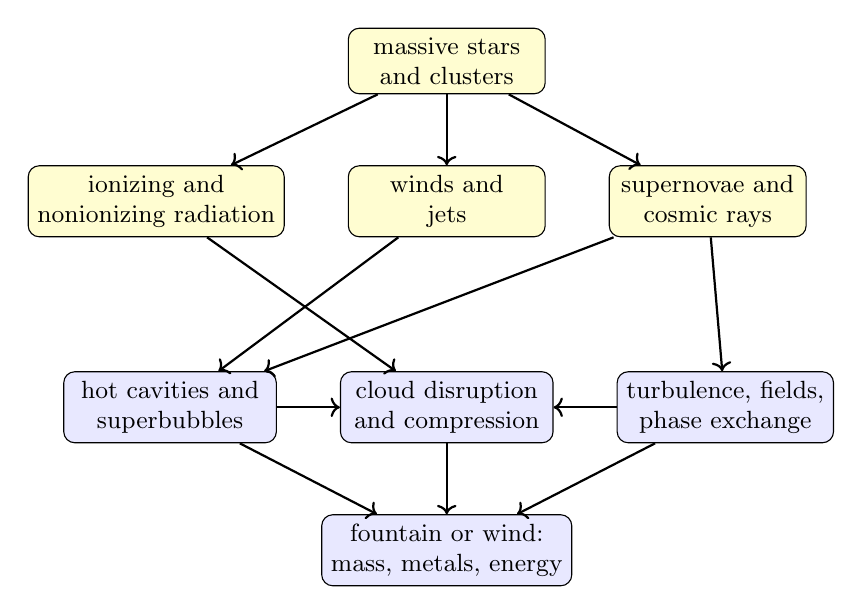
\begin{tikzpicture}[
 node distance=9mm and 8mm,
 every node/.style={font=\small},
 source/.style={draw,rounded corners,fill=yellow!18,align=center,minimum width=25mm},
 phase/.style={draw,rounded corners,fill=blue!9,align=center,minimum width=27mm},
 arrow/.style={->,thick}
]
 \node[source] (stars) {massive stars\\and clusters};
 \node[source,below left=of stars] (rad) {ionizing and\\nonionizing radiation};
 \node[source,below=of stars] (winds) {winds and\\jets};
 \node[source,below right=of stars] (sn) {supernovae and\\cosmic rays};
 \node[phase,below=17mm of winds] (cloud) {cloud disruption\\and compression};
 \node[phase,left=of cloud] (hot) {hot cavities and\\superbubbles};
 \node[phase,right=of cloud] (turb) {turbulence, fields,\\phase exchange};
 \node[phase,below=of cloud] (out) {fountain or wind:\\mass, metals, energy};
 \draw[arrow] (stars)--(rad); \draw[arrow] (stars)--(winds); \draw[arrow] (stars)--(sn);
 \draw[arrow] (rad)--(cloud); \draw[arrow] (winds)--(hot); \draw[arrow] (sn)--(hot);
 \draw[arrow] (sn)--(turb); \draw[arrow] (hot)--(cloud); \draw[arrow] (turb)--(cloud);
 \draw[arrow] (hot)--(out); \draw[arrow] (cloud)--(out); \draw[arrow] (turb)--(out);
\end{tikzpicture}
\caption{Original feedback coupling map.  Arrows represent transfer, not a strict
time sequence.  Observed phases exchange mass and energy, so summing independently
derived phase rates can double count the same material.}
\label{fig:feedback-coupling-map}
\end{figure}

\section{Cosmic rays and magnetic coupling}

Supernova shocks and other accelerators populate nonthermal particles.  Cosmic rays
contribute pressure, ionize shielded gas, heat through wave damping, and can drive
outflows if their pressure gradient couples to plasma.  Transport may involve
advection, diffusion, and streaming, each anisotropic in an ordered magnetic field.

Gamma rays probe hadronic interactions and energetic particles; synchrotron emission
depends on electron spectra and magnetic field; ion chemistry constrains low-energy
ionization.  These observables sample different portions of the cosmic-ray spectrum.
A single ``cosmic-ray energy density'' inferred from radio equipartition is not a
direct measurement of the particles that dominate molecular ionization.

Cosmic-ray-driven winds can accelerate gas more gradually than a purely thermal wind
and may remain effective where radiative cooling removes thermal energy.  Quantitative
predictions depend on transport coefficients and wave damping, which are not universal
constants.  Line diagnostics of ionization state, temperature, and kinematics provide
important indirect constraints.

\section{How multiphase outflows are observed}

Different tracers select different phases and geometries:
\begin{table}[tbp]
\centering
\caption{Outflow tracers and principal selection effects.}
\label{tab:outflow-tracers}
\begin{tabularx}{\textwidth}{@{}
 >{\raggedright\arraybackslash}p{0.19\textwidth}
 >{\raggedright\arraybackslash}p{0.27\textwidth}
 >{\raggedright\arraybackslash}X@{}}
\toprule
Phase or component & Representative diagnostics & Main selection effects \\
\midrule
Hot volume-filling wind & X-ray continuum and highly ionized lines & Emission weights
dense interfaces; absorption requires a bright background; temperature and abundance
degenerate with emission measure \\
Warm ionized & H$\alpha$, [N\,II], [S\,II], [O\,III], UV ions & Extinction, shocks
versus photoionization, density-squared weighting, projection and beam smearing \\
Warm neutral & Na\,I D, Mg\,II, H\,I absorption and emission & Resonant scattering,
stellar contamination, ionization/depletion corrections, covering fraction \\
Molecular & CO, OH, HCN, HCO$^+$, warm H$_2$ & Conversion factor, excitation,
opacity, abundance, interferometric filtering, orientation \\
Dusty gas & Far-IR continuum, extinction, scattered light & Dust temperature,
opacity, dust-to-gas ratio, foreground versus outflow geometry \\
Cosmic rays & Synchrotron, gamma rays, ionization chemistry & Magnetic field,
transport, loss time, unrelated AGN contribution \\
\bottomrule
\end{tabularx}
\end{table}

Absorption detects only gas projected against a background source, yielding a
covering-weighted pencil beam.  Emission can map the flow but strongly weights dense
clumps.  Resonant emission may be scattered into locations far from photon production.
Agreement of velocity alone does not prove that phases are co-spatial.

\section{Mass, momentum, and energy of an outflow}

For an ionized phase whose recombination luminosity is
$L\propto n_en_pV$, mass scales as
\begin{equation}
 M_{\rm ion}\simeq
 \frac{\mu m_{\rm H}L_{\rm rec}}
 {h\nu\alpha^{\rm eff}(T)n_e},
 \label{eq:ionized-outflow-mass}
\end{equation}
after extinction and contamination corrections.  Density uncertainty maps directly
to mass uncertainty.  Density-sensitive doublets often measure bright clumps rather
than the low-density material that may dominate volume or mass.

For a thin partial shell at radius $R$ subtending solid angle $\Omega$, an absorption
column gives
\begin{equation}
 M_{\rm shell}\simeq\Omega R^2\mu m_{\rm H}N_{\rm H},
 \label{eq:shell-mass-column}
\end{equation}
where $N_{\rm H}$ requires ionization, abundance, depletion, and covering corrections.
The radius is often the least directly constrained quantity for unresolved absorption.

Several incompatible conventions are used for outflow rate.  For a shell crossing
time $R/v$,
\begin{equation}
 \dot M_{\rm out}\simeq\frac{M_{\rm out}v}{R}.
 \label{eq:outflow-rate-thin-shell}
\end{equation}
A uniformly filled steady cone may introduce a factor of order a few.  Rather than
calling one convention correct in every geometry, authors should provide $M$, $v$,
$R$, and the exact equation so readers can translate.

Velocity choices are likewise consequential.  A centroid measures bulk shift; a
maximum or percentile velocity emphasizes wings; deprojected speed depends on cone
inclination.  Because energy scales as $v^2$, wing definitions dominate kinetic-power
comparisons.

\subsection{Worked example: geometry dominates an outflow rate}

Suppose a molecular outflow has $M_{\rm out}=10^8M_\odot$, characteristic speed
$v=300\,\mathrm{km\,s^{-1}}$, and radius $R=1$~kpc.  The flow-time estimate is
\begin{equation}
 \dot M_{\rm out}\simeq31
 \left(\frac{M_{\rm out}}{10^8M_\odot}\right)
 \left(\frac{v}{300\,\mathrm{km\,s^{-1}}}\right)
 \left(\frac{R}{1\,\mathrm{kpc}}\right)^{-1}
 M_\odot\,\mathrm{yr^{-1}}.
\end{equation}
If the emission is actually concentrated at 0.3~kpc, the rate rises by more than a
factor of three.  If the molecular conversion factor shifts by a factor of four, so
does the rate.  A formal line-flux uncertainty of five percent is not the relevant
total uncertainty.

\section{Launch, survival, and phase creation}

Cool clouds placed in a fast hot wind experience ram pressure, shocks, shear, thermal
conduction, magnetic draping, and radiative cooling.  A characteristic cloud-crushing
time is
\begin{equation}
 t_{\rm cc}=\frac{\chi^{1/2}r_c}{v_{\rm rel}},
 \label{eq:cloud-crushing-time}
\end{equation}
where $\chi=\rho_c/\rho_h$.  In simple nonradiative hydrodynamics, disruption can occur
before acceleration to the hot-wind speed.  Radiative cooling in mixed gas, magnetic
fields, conduction, self-gravity, and continuous cloud creation can extend survival
or create new cool material in situ.

Therefore cool gas at large radius need not be the same parcels launched cold from
the disk.  It may have condensed from a mixed outflow.  Metallicity, dust survival,
ion ratios, cloud size distribution, and velocity alignment can test origin, but no
single diagnostic is decisive.

\section{Escape, fountains, and recycling}

Comparing line-of-sight velocity with an escape speed is only a first check.  The gas
has a three-dimensional velocity distribution, the gravitational potential evolves,
and hydrodynamic drag, cooling, and pressure forces continue after observation.  A
parcel below local escape speed can be accelerated; one above it can transfer energy
and fall back.

Material that returns in a galactic fountain still matters: it redistributes metals
and angular momentum, exchanges mass with the halo, and delays star formation.  The
CGM can contain first-time inflow, recycled wind, stripped satellite gas, and material
circulating within the halo \citep{TumlinsonPeeplesWerk2017}.  An absorption component
labeled ``outflow'' from its velocity sign alone may be ambiguous without galaxy
orientation and systemic-velocity precision.

\section{A rigorous feedback claim}

A strong feedback analysis proceeds through five tests:
\begin{enumerate}
 \item \textbf{Identification:} show that the spectral component is distinct from
rotation, tidal structure, beam smearing, and unrelated foreground gas.
 \item \textbf{Excitation:} determine whether photoionization, shocks, mixing, or an
AGN supplies the observed lines; allow mixtures.
 \item \textbf{Geometry:} state the aperture, radius, solid angle, inclination,
covering fraction, and whether absorption and emission sample the same structure.
 \item \textbf{Budget:} derive mass, momentum, and energy with conversion-factor,
density, ionization, extinction, and phase corrections made explicit.
 \item \textbf{Causality and fate:} compare source history with flow time and assess
whether gas is dispersed, recycled, or escaping rather than equating detection with
quenching.
\end{enumerate}

The ideal output is not one ``feedback efficiency'' with a tiny statistical error.
It is a phase-resolved budget with transparent conditional ranges.  Such a budget can
be compared meaningfully with simulations, which must apply the same apertures, line
emissivities, and selection functions to their synthetic observations.

\chapter{The Circumgalactic Medium, the Intergalactic Medium, and the Cosmic Web}
\label{chap:cgm-igm}

\section{A working map of diffuse baryons}

The gaseous Universe is not naturally divided into boxes. Gas crosses the
interstellar medium (ISM), circumgalactic medium (CGM), intragroup medium, and
intergalactic medium (IGM); the same parcel may be accreted, form stars, be
ejected, cool, mix, and return. The names are nevertheless useful if they are
treated as operational definitions rather than immutable phases. In this
chapter, the \emph{CGM} is gas outside the bright stellar body and cold
star-forming disk but inside the region dynamically associated with a galaxy's
dark-matter halo. The \emph{IGM} is gas outside individual halos. The
\emph{cosmic web} is the evolving network of sheets, filaments, nodes, and
voids created by gravitational instability. These definitions deliberately
leave a transition zone: around groups, interacting systems, and splashback
regions, assignment to one galaxy can be physically ambiguous
\citep{Tumlinson2017,FaucherGiguereOh2023}.

A convenient halo scale is defined by
\begin{equation}
 M_{\Delta}=\frac{4\pi}{3}\,\Delta\,\rho_{\rm ref}(z)R_{\Delta}^{3},
 \label{eq:halo-definition}
\end{equation}
where the reference density may be the critical or mean matter density.
Authors who quote $R_{200\rm c}$, $R_{200\rm m}$, or a "virial radius" are
not necessarily using the same boundary. The conversion can be tens of
percent and should never be hidden when normalizing impact parameters.
Associated velocity and temperature scales are
\begin{align}
 V_{\Delta} &= \left(\frac{GM_{\Delta}}{R_{\Delta}}\right)^{1/2},\\
 T_{\rm vir} &\simeq \frac{\mu m_{\rm p}V_{\Delta}^{2}}{2k_{\rm B}},
 \label{eq:tvir}
\end{align}
with mean molecular weight $\mu$. For an ionized, Milky-Way-mass halo,
$T_{\rm vir}$ is of order $10^{6}$ K. This number is a guide, not a claim
that the halo is isothermal.

The most important conceptual correction to a one-phase cartoon is that
temperature labels do not define unique structures. "Cool" gas near
$10^{4}$ K may occur in infalling filaments, stripped satellite wakes,
radiatively cooled wind material, turbulent mixing layers, or self-shielded
clouds. "Warm" gas near $10^{5}$--$10^{6}$ K may be cooling through a
short-lived temperature interval rather than occupying a stable volume.
"Hot" gas can be supported approximately hydrostatically, driven by winds,
or shock heated during accretion. Observed velocity coincidence between two
ions does not prove that they are co-spatial. A spectrograph collapses a
three-dimensional, time-dependent medium into optical depth versus one
velocity coordinate.

\section{Why the CGM is central to galaxy evolution}

A galaxy's stellar mass is only the integrated residue of a larger baryon
cycle. Cosmological inflow supplies gas; cooling and angular-momentum
transport deliver some of it to the ISM; stars and black holes return mass,
metals, momentum, cosmic rays, and radiation; satellites donate gas by winds
and stripping; and some material escapes or is exchanged between halos.
Consequently, the CGM is simultaneously a fuel reservoir, a feedback
calorimeter, and a record of environmental processing
\citep{Tumlinson2017,FaucherGiguereOh2023,Hafen2019}.

For a control surface at radius $r$, a formal instantaneous mass flux is
\begin{equation}
 \dot{M}(r)=\int \rho(\boldsymbol{x})
        \left[\boldsymbol{v}(\boldsymbol{x})-\boldsymbol{v}_{\rm frame}\right]
        \cdot \hat{\boldsymbol{r}}\,r^{2}\,{\rm d}\Omega .
 \label{eq:mass-flux}
\end{equation}
This equation is straightforward in a simulation and extremely difficult to
infer from a single sightline. An absorber supplies a column density and a
line-of-sight velocity, but generally not its distance along the sightline,
solid angle, transverse velocity, or time history. Thus labels such as
"inflow" and "outflow" should be probabilistic unless geometry supplies
additional evidence. Major-axis/minor-axis trends, metallicity, comparison
with the escape speed, resolved emission, or multiple nearby sightlines can
strengthen the interpretation, but none is individually decisive.

The cool-CGM mass inferred from absorption illustrates the inference chain.
For a hydrogen column profile $N_{\rm H}(R)$ and azimuthal covering fraction
$f_{\rm c}(R)$,
\begin{equation}
 M_{\rm cool}(<R_{\rm max}) =
 2\pi \mu_{\rm H}m_{\rm p}
 \int_{0}^{R_{\rm max}} N_{\rm H}(R) f_{\rm c}(R)R\,{\rm d}R .
 \label{eq:cgm-mass}
\end{equation}
The directly constrained quantity is often $N_{\rm H\,I}$, not $N_{\rm H}$.
Writing $f_{\rm H\,I}=N_{\rm H\,I}/N_{\rm H}$ gives
$N_{\rm H}=N_{\rm H\,I}/f_{\rm H\,I}$. The neutral fraction can be tiny and
depends on density, spectrum and amplitude of the ionizing field, temperature,
shielding, and non-equilibrium history. Large masses inferred for cool halo
gas are therefore important but model conditioned
\citep{Werk2014,Prochaska2017}. A robust paper reports which part of
Equation~\ref{eq:cgm-mass} is measured and which part is assumed.

\section{Thermal competition and multiphase structure}

Two timescales provide a useful first organization. An approximate radiative
cooling time is
\begin{equation}
 t_{\rm cool} \simeq
 \frac{\tfrac{3}{2}n_{\rm tot}k_{\rm B}T}
      {n_{\rm e}n_{\rm H}\Lambda(T,Z,J_{\nu})},
 \label{eq:cooling-time}
\end{equation}
where $\Lambda$ includes radiative losses and, if desired, photoheating. A
local free-fall estimate is
\begin{equation}
 t_{\rm ff}(r)=\left[\frac{2r}{g(r)}\right]^{1/2}.
 \label{eq:freefall}
\end{equation}
When shock-heated gas cools slowly compared with its dynamical time, an
extended hot atmosphere can persist. When cooling is rapid, cold streams,
condensation, and radiative interfaces become important. The ratio
$t_{\rm cool}/t_{\rm ff}$ is a diagnostic, not a universal one-number
criterion; rotation, turbulence, uplift, conduction, magnetic topology,
cosmic-ray pressure, and ongoing forcing all alter the outcome
\citep{FaucherGiguereOh2023}.

Pressure balance is similarly informative but not guaranteed:
\begin{equation}
 P_{\rm tot}=P_{\rm th}+P_{\rm turb}+P_{\rm B}+P_{\rm CR}+\cdots .
\end{equation}
A cool component can have $n_{\rm cool}T_{\rm cool}\neq
n_{\rm hot}T_{\rm hot}$ while remaining confined by non-thermal pressure,
ram pressure, gravity, or time dependence. An apparent pressure discrepancy
between photoionization models and a coronal model may therefore diagnose
missing physics, but it may also expose an incorrect ionizing background or
an assumption that non-coincident velocity components form one cloud.

Interfaces are disproportionately visible. Conductive boundaries,
radiative shocks, and turbulent mixing can generate ions such as
$\mathrm{C\,IV}$, $\mathrm{N\,V}$, $\mathrm{O\,VI}$, and
$\mathrm{Ne\,VIII}$ while containing little of the total mass. In
collisional ionization equilibrium, each ion fraction has a characteristic
temperature range, but gas that cools faster than it recombines retains an
ionization memory. Photoionization can also produce high ions at much
lower kinetic temperature if the density is sufficiently small. Ion names
are therefore not thermometers by themselves
\citep{GnatSternberg2007,SutherlandDopita1993}.

\section{A tracer ladder for circumgalactic gas}

\subsection{Neutral hydrogen}

$\mathrm{H\,I}$ is usually the entry point because the Lyman series spans an
enormous range of column density. Ly$\alpha$ is sensitive but saturates
readily. Higher-order Lyman lines have smaller oscillator strengths and
recover information hidden in saturated Ly$\alpha$. At sufficiently high
$N_{\rm H\,I}$, the continuum optical depth at the Lyman edge,
\begin{equation}
 \tau_{912}=N_{\rm H\,I}\sigma_{912},
\end{equation}
constrains the neutral column even when line cores are black. At still larger
columns, Lorentzian damping wings determine $N_{\rm H\,I}$. The lesson is to
design coverage of a \emph{ladder}, not a single line.

Absorber names encode approximate column regimes, but boundaries vary with
author and purpose. The Ly$\alpha$ forest generally denotes mostly
photoionized systems below the classical Lyman-limit threshold. Partial
Lyman-limit systems and Lyman-limit systems occupy the transition to optical
thickness near 1 Ryd. Sub-damped and damped Ly$\alpha$ systems contain
progressively larger neutral columns; the conventional DLA boundary is
$N_{\rm H\,I}=2\times10^{20}\ {\rm cm^{-2}}$
\citep{Wolfe2005}. These are observational classes, not one-to-one maps onto
IGM, CGM, and ISM.

\subsection{Low and intermediate ions}

$\mathrm{Mg\,II}$, $\mathrm{C\,II}$, $\mathrm{Si\,II}$,
$\mathrm{Fe\,II}$, and $\mathrm{O\,I}$ preferentially trace cool or
low-ionization material. Their diagnostic value differs:
\begin{itemize}
  \item $\mathrm{O\,I}$ is coupled to $\mathrm{H\,I}$ by charge exchange over
  useful conditions, making O/H comparatively direct in neutral gas.
  \item $\mathrm{Si\,II}$ and $\mathrm{Fe\,II}$ have several transitions
  spanning oscillator strengths, valuable for diagnosing saturation.
  \item Refractory Fe and Si can be depleted onto dust, so gas-phase abundance
  ratios need not equal nucleosynthetic ratios.
  \item Mg II is observable from the ground after modest redshifting and has
  built large statistical samples, but equivalent width mixes column,
  velocity spread, covering fraction, and saturation.
\end{itemize}

Intermediate ions such as $\mathrm{Si\,III}$ and $\mathrm{C\,III}$ are often
strong because they can be abundant in photoionized gas, but their strongest
transitions saturate easily. A precise equivalent width is not necessarily a
precise column density.

\subsection{High ions and hot gas}

$\mathrm{C\,IV}$, $\mathrm{N\,V}$, $\mathrm{O\,VI}$, and
$\mathrm{Ne\,VIII}$ probe harder ionization conditions and often reveal
interfaces or warm-hot gas. O VI is especially important because its
$1031.93$ and $1037.62$ \AA\ doublet is accessible to far-UV spectroscopy at
low redshift and to optical spectroscopy at sufficiently high redshift.
Strong, extended O VI around star-forming galaxies established a major metal
reservoir \citep{Tumlinson2011}. Yet converting $N_{\rm O\,VI}$ into oxygen
or total gas mass requires both the ion fraction $f_{\rm O\,VI}$ and
metallicity:
\begin{equation}
 N_{\rm H} =
 \frac{N_{\rm O\,VI}}
 {f_{\rm O\,VI}\,({\rm O/H})_{\odot}\,10^{[{\rm O/H}]}} .
 \label{eq:ovi-correction}
\end{equation}
A factor-of-ten uncertainty in metallicity becomes a factor-of-ten
uncertainty in mass.

At $T\gtrsim10^{6}$ K, abundant ions emit and absorb soft X-rays. Oxygen
$\mathrm{O\,VII}$ and $\mathrm{O\,VIII}$ are central WHIM and halo tracers;
the Fe-L complex diagnoses hotter, metal-rich plasma. Emission scales
approximately as $\int n_{\rm e}n_{\rm H}\Lambda_E\,{\rm d}\ell$ and is
weighted toward dense clumps. Absorption scales as $\int n_i\,{\rm d}\ell$
and is more sensitive to diffuse columns but requires an exceptionally bright
background source and exquisite control of instrumental structure. The two
methods do not sample the same density weighting.

\section{The IGM as a fluctuating medium}

\subsection{Photoionized forest}

The classical cloud picture has largely been replaced by a continuous-density
view. Much Ly$\alpha$ forest absorption arises in mildly overdense,
photoionized sheets and filaments whose peculiar velocities, temperature,
thermal broadening, and Hubble expansion shape the spectrum
\citep{Rauch1998,McQuinn2016}. For highly ionized hydrogen in equilibrium,
\begin{equation}
 n_{\rm H\,I}\Gamma_{\rm H\,I}
 \simeq n_{\rm e}n_{\rm p}\alpha_{\rm A}(T),
 \label{eq:photoequilibrium}
\end{equation}
so the neutral fraction is extremely sensitive to the photoionization rate
$\Gamma_{\rm H\,I}$ and moderately sensitive to temperature through the
recombination coefficient. The transmitted flux is
\begin{equation}
 F(v)=C(v)\exp[-\tau(v)]+N(v),
 \label{eq:forest-flux}
\end{equation}
with continuum $C$, absorption field $\tau$, and noise $N$. In forest
cosmology, continuum fitting is not merely cosmetic: fitting away
long-wavelength modes distorts the measured correlation function and must be
represented in the forward model.

A useful analytic argument sets an absorber's characteristic scale near a
local Jeans or filtering scale. Combining photoionization equilibrium with
that scale produces a relation between $N_{\rm H\,I}$ and gas overdensity
\citep{Schaye2001}. The relation explains why the column-density distribution
can encode the matter distribution, but its coefficients depend on
temperature, ionizing background, gas fraction, and dynamical assumptions.
It should be used as a calibrated scaling, not an exact cloud ruler.

\subsection{Mean opacity, thermal history, and reionization}

Even a small neutral fraction produces substantial Ly$\alpha$ opacity because
the transition is strong. The Gunn--Peterson argument therefore constrains
diffuse neutral hydrogen far below the fraction needed for a predominantly
neutral Universe \citep{GunnPeterson1965}. A dark trough at high redshift does
not by itself measure a unique neutral fraction: once Ly$\alpha$ saturates,
small changes in transmission can correspond to a broad range of neutral
fractions. Higher Lyman lines, damping-wing shape, proximity-zone structure,
and ensembles of sightlines are needed.

The forest also remembers heat input. Photoheating during hydrogen and
helium reionization establishes a temperature--density relation often written
\begin{equation}
 T(\Delta)=T_0\Delta^{\gamma-1},
\end{equation}
for a restricted low-density regime, where
$\Delta=\rho_{\rm b}/\bar{\rho}_{\rm b}$. Thermal broadening, pressure
smoothing, and peculiar velocities affect line widths and small-scale flux
power differently. Inferring $T_0$ and $\gamma$ therefore requires synthetic
spectra with the instrumental line-spread function and the same continuum and
masking operations as the data.

\subsection{The warm-hot IGM}

As large-scale structure grows, accretion and merger shocks heat some diffuse
gas to $10^{5}$--$10^{7}$ K, the conventionally defined warm-hot
intergalactic medium (WHIM) \citep{CenOstriker1999,Dave2001}. No single tracer
is complete:
\begin{description}
  \item[Broad Ly$\alpha$ absorbers] are metallicity independent in principle,
  but blends, continuum errors, and non-thermal broadening can mimic large
  Doppler parameters.
  \item[O VI and Ne VIII] are powerful in the UV, but their baryon conversion
  depends on metallicity and ionization history.
  \item[O VII and O VIII] access hotter gas in X-rays, but line equivalent
  widths are tiny and claimed detections demand independent confirmation,
  careful trials accounting, and stable calibration.
  \item[Thermal Sunyaev--Zel'dovich and dispersion measures] respond to
  electrons rather than a metal abundance, but projection and halo separation
  are nontrivial.
\end{description}
Historically, "missing baryons" has meant baryons permitted by early-Universe
constraints but absent from low-redshift inventories, not non-baryonic dark
matter. Census estimates evolve with surveys and ionization corrections
\citep{Bregman2007,Shull2012,PerouxHowk2020}. Individual X-ray WHIM claims,
including influential O VII results, should be presented with their stated
significance and subsequent replication status rather than as closure of the
census \citep{Nicastro2018}.

\section{Metals as history, not merely abundance}

Metals in diffuse gas prove prior processing by stars, but translating them
into a transport history is difficult. The logarithmic abundance is
\begin{equation}
 [{\rm X/H}]=
 \log_{10}\left(\frac{N_{\rm X}}{N_{\rm H}}\right)
 -\log_{10}\left(\frac{\rm X}{\rm H}\right)_{\odot},
 \label{eq:metallicity}
\end{equation}
after ionization and depletion corrections. The adopted solar reference
must be stated \citep{Asplund2021}. A metallicity posterior inherits
uncertainty from $N_{\rm H\,I}$, the radiation field, gas density, relative
abundance pattern, dust depletion, phase assignment, and atomic data.

Low metallicity can support an accretion interpretation, while enhanced
$\alpha$/Fe or N/O can encode enrichment timescales. However, metal-poor gas
may be old IGM material mixed only weakly with winds; metal-rich gas may arise
from outflow, recycling, stripping, or enrichment by another galaxy.
Metallicity alone does not provide the sign of radial velocity. Observed
metallicity distributions are also selection functions: metal-selected
samples and H I-selected samples answer different questions. Early evidence
for a bimodal low-redshift Lyman-limit metallicity distribution was
scientifically influential \citep{Lehner2013}; later analyses should be
compared at matched H I range, redshift, sensitivity, and priors rather than
reduced to a slogan.

\section{From pencil beams to maps}

Absorption is extraordinarily sensitive because detectability does not suffer
the same density-squared penalty as emission, but it sparsely samples the sky.
Emission maps morphology but is surface-brightness limited and vulnerable to
sky subtraction, scattered light, and resonant transfer. The strongest
programs combine:
\begin{enumerate}
  \item a background quasar or galaxy grid for column density and kinematics;
  \item deep galaxy redshifts to establish environment and impact parameters;
  \item integral-field emission mapping for morphology and velocity;
  \item X-ray, millimeter, or radio measurements for phases missed in the UV;
  \item synthetic observations of simulations passed through the same
  selection, resolution, and noise.
\end{enumerate}

At high redshift, extended Ly$\alpha$ emission can illuminate cool gas around
galaxies and quasars. Ly$\alpha$ is resonant: a photon can emerge far from
where it was produced and at a frequency altered by scattering through a
moving medium. Morphology and line centroid therefore cannot be read as a
direct emissivity or velocity map without radiative-transfer modeling.
Non-resonant recombination lines and metal lines provide critical controls.

Dense background-source fields enable tomography. Each sightline remains a
one-dimensional convolution of density, ionization, peculiar velocity, and
thermal state, but regularized reconstruction can reveal coherent filaments
and voids. On much larger scales, surveys treat transmitted forest flux as a
biased tracer and measure its auto-correlation and cross-correlation with
quasars. DESI has demonstrated the statistical power of hundreds of
thousands of forest spectra for baryon acoustic oscillations
\citep{DESI2025LyA}. This regime is conceptually continuous with single-line
analysis: both require a forward model for the continuum, absorption,
instrument, masking, and selection.

\section{A disciplined interpretation protocol}

For any diffuse-gas claim, write the chain in the following order.
\begin{enumerate}
  \item \textbf{Observed:} normalized flux, surface brightness, equivalent
  width, profile shape, angular separation, and their covariance.
  \item \textbf{Instrumental:} spectral and spatial line-spread functions,
  wavelength zero point, sensitivity, background model, detector artifacts,
  aperture, and completeness.
  \item \textbf{Atomic inference:} transition identity, oscillator strength,
  column density, excitation, saturation assessment, and blend model.
  \item \textbf{Plasma inference:} ionization mechanism, density,
  temperature, radiation field, abundance pattern, depletion, and phase
  association.
  \item \textbf{Geometric inference:} distance, path length, covering
  fraction, opening angle, inclination, and association with a galaxy or
  filament.
  \item \textbf{Derived physics:} total mass, flux, cooling rate, metal mass,
  energy, and comparison with binding or feedback budgets.
\end{enumerate}
Uncertainty normally grows down this list. Reporting a precise equivalent
width with a loosely constrained total mass is not contradictory; it is an
honest consequence of the inference hierarchy.

\section{Common category errors}

\begin{itemize}
  \item \textbf{Ion equals phase.} O VI can arise from collisionally ionized,
  photoionized, non-equilibrium cooling, or mixed gas.
  \item \textbf{Velocity equals radial motion.} A blueshift is not
  automatically an outflow if systemic redshift, inclination, rotation, and
  environment are uncertain.
  \item \textbf{Equivalent width equals column.} Saturated equivalent width
  can increase through velocity spread with little sensitivity to column.
  \item \textbf{Emission and absorption sample the same gas.} Their density
  weighting and selection functions differ.
  \item \textbf{A halo boundary is observed.} $R_{\rm vir}$ is convention and
  model; gas dynamics need not change abruptly there.
  \item \textbf{Metallicity is origin.} Enrichment constrains history but
  rarely identifies a unique transport channel.
  \item \textbf{A simulation cell is a cloud.} Numerical resolution, mixing,
  and subgrid feedback can alter synthetic absorber structure; convergence of
  galaxy properties does not guarantee convergence of CGM interfaces.
\end{itemize}

\section{Research frontiers}

Several measurements would transform the field. Closely spaced sightlines
can determine transverse coherence and cloud sizes without assuming a path
length. Joint UV and X-ray spectroscopy can connect cool, interface, and
virial-temperature gas. Deep, absolutely calibrated emission mapping can
measure faint cooling and fluorescence. Time-domain absorption against
moving or variable background sources can probe small-scale structure.
Finally, hierarchical analyses that fit populations rather than one absorber
at a time can propagate non-detections, selection functions, ionizing-field
uncertainty, and halo-to-halo scatter.

The central scientific target is not a census of ion labels. It is a
quantitative account of how mass, metals, momentum, and energy move between
galaxies and the cosmic web. Spectral lines are the measuring apparatus, and
their greatest power comes from combining transitions whose degeneracies are
different.

\chapter{Absorption-Line Spectroscopy: From Pixels to Physical Gas}
\label{chap:absorption}

\section{What an absorption spectrum actually measures}

An absorption spectrum is a comparison between received flux and an estimate
of the flux that would have been received without the absorber. In its most
useful forward form,
\begin{equation}
 F_{\rm pix}(\lambda)=
 \left\{
 C(\lambda)\left[(1-C_{\rm f})+
 C_{\rm f}\exp\left(-\sum_k\tau_k(\lambda)\right)\right]
 \right\}\otimes {\cal L}(\lambda)
 +B(\lambda)+\epsilon(\lambda),
 \label{eq:abs-forward}
\end{equation}
where $C$ is the source continuum and broad emission spectrum, $C_{\rm f}$ is
the covering fraction, $\mathcal{L}$ is the instrumental line-spread function
(LSF), $B$ is any residual background or scattered light, and $\epsilon$ is
noise. Each physical velocity component and each blended transition
contributes an optical-depth profile $\tau_k$. Equation~\ref{eq:abs-forward}
is a reminder that a fitted Voigt component is not directly observed. The
detector records a sampled convolution of source, absorber, instrument, and
background.

For an intervening quasar absorber the covering fraction is often taken as
unity, but this should not become reflex. Partial coverage is common in
intrinsic AGN absorption, stellar winds, compact continuum sources occulted by
small clouds, and spatially mixed emission/absorption. A nonzero flux floor in
a strong doublet can arise from partial coverage, unresolved velocity
structure, scattered light, an erroneous background, or unrelated emission.
The competing explanations must be fitted at the flux level.

The line identification itself is a hypothesis. A persuasive identification
uses multiple transitions at one redshift, expected strength ordering, absence
of plausible alternatives, and consistency with instrumental coverage.
Atomic wavelengths and oscillator strengths must come from a versioned source
such as \citet{Morton2003}; precision claims should not mix air and vacuum
wavelengths or oscillator-strength compilations silently.

\section{Coordinates, frames, and velocity conventions}

The first redshift estimate is
\begin{equation}
 1+z = \frac{\lambda_{\rm obs}}{\lambda_0}
     = \frac{\nu_0}{\nu_{\rm obs}}.
 \label{eq:redshift}
\end{equation}
For velocity structure within a system, define the convention explicitly. A
commonly used local coordinate about reference redshift $z_{\rm ref}$ is
\begin{equation}
 v=c\,\frac{z-z_{\rm ref}}{1+z_{\rm ref}}.
 \label{eq:local-velocity}
\end{equation}
At large offsets, use the exact relativistic relation or work directly in
redshift. Wavelength calibration must also specify frame: observatory,
heliocentric, barycentric, Local Standard of Rest, or a galaxy systemic frame.
Optical, radio, and relativistic velocity definitions differ at non-negligible
redshift. Combining UV, optical, and radio spectra without harmonizing
definitions can manufacture offsets comparable to the line widths being
interpreted.

The adopted systemic redshift often dominates an outflow velocity's
uncertainty, especially if it comes from a broad or asymmetric line. Narrow
stellar absorption, molecular lines, or spatially integrated nebular emission
may each define a different practical zero point.

\section{Continuum placement is part of the inference}

Dividing by a single best continuum and forgetting its uncertainty produces
overconfident line measurements. The preferred approach is to model local
continuum parameters jointly with the absorption. For an isolated line, a
low-order polynomial or spline over windows demonstrably free of absorption
may suffice. For a quasar Ly$\alpha$ forest, broad emission complexes and
correlated forest absorption require a global template, principal components,
Gaussian process, or forward model. For galaxy spectra, stellar photospheric
features and the instrumental response may be comparable to the interstellar
line.

Continuum choices should be tested by:
\begin{enumerate}
  \item changing the fit-window boundaries;
  \item increasing or decreasing continuum flexibility;
  \item injecting synthetic lines into unnormalized data;
  \item propagating continuum samples into equivalent width and column
  posteriors;
  \item checking blank regions for biased residuals and underestimated
  covariance.
\end{enumerate}
For broad, shallow features, continuum uncertainty can dominate photon noise.
A claimed broad Ly$\alpha$ absorber or AGN trough is not secure if it
disappears under plausible continuum models.

\section{Equivalent width: robust summary, incomplete physics}

For continuum-normalized flux $F_n(\lambda)$, the observed-frame equivalent
width is
\begin{equation}
 W_{\lambda,\rm obs}=\int_{\lambda_1}^{\lambda_2}
       \left[1-F_n(\lambda)\right]\,{\rm d}\lambda,
 \qquad
 W_{\lambda,\rm r}=\frac{W_{\lambda,\rm obs}}{1+z}.
 \label{eq:abs-equivalent-width}
\end{equation}
Equivalent width is conserved by a normalized LSF when all absorbed flux is
included and the continuum is correct. This makes it useful at modest
resolution. It does not make it a unique measure of column density.

In the optically thin regime, the rest equivalent width satisfies
\begin{equation}
 N\,[{\rm cm^{-2}}] =
 1.13\times10^{20}\,
 \frac{W_{\lambda,\rm r}\,[\text{\AA}]}
      {f\lambda_0^2\,[\text{\AA}^2]},
 \label{eq:abs-linear-cog}
\end{equation}
where $f$ is the oscillator strength. Once the line saturates, equivalent
width becomes sensitive mainly to Doppler width and component spread.
Eventually damping wings restore a strong column dependence. These are the
linear, saturated, and damping portions of the curve of growth
\citep{Spitzer1978,Draine2011}.

For a pixel sum with independent errors, a simple statistical variance is
\begin{equation}
 \sigma^2(W_\lambda)
 =\sum_i \left(\Delta\lambda_i\,\sigma_{F_n,i}\right)^2,
\end{equation}
but reduced spectra often have correlated noise from resampling, flat fields,
and background subtraction. Continuum uncertainty, integration-window
uncertainty, fixed-pattern noise, and blends must be added or marginalized.
An empirical distribution from line-free windows with the same width is often
more realistic than a diagonal-noise formula.

\section{Optical depth and column density}

\subsection{The apparent-optical-depth method}

For full coverage and a reliable continuum, define
\begin{equation}
 \tau_{\rm a}(v)=\ln\left[\frac{1}{F_n(v)}\right].
 \label{eq:aod-tau}
\end{equation}
The apparent column density per unit velocity is
\begin{equation}
 N_{\rm a}(v)=
 \frac{m_{\rm e}c}{\pi e^2}\frac{\tau_{\rm a}(v)}{f\lambda_0}
 =3.768\times10^{14}
 \frac{\tau_{\rm a}(v)}
      {f\lambda_0[\text{\AA}]}
 \frac{{\rm cm^{-2}}}{{\rm km\,s^{-1}}}.
 \label{eq:abs-aod-column}
\end{equation}
Integrating over velocity gives $N_{\rm a}$. The method preserves kinematic
information and enables a direct saturation test: two transitions of the same
ion should yield the same $N_{\rm a}(v)$ when resolved and unsaturated
\citep{SavageSembach1991}.

If the stronger transition yields systematically smaller $N_{\rm a}(v)$ than
the weaker one, unresolved saturation is likely. Equality is necessary but
not always sufficient: both transitions can be severely saturated and
unresolved. Negative fluxes, low signal-to-noise, and logarithmic
transformation introduce biases; simulations tailored to the data help
quantify them \citep{Fox2005}. Report lower limits rather than forcing a
precise column from black cores.

\subsection{Voigt profiles}

The intrinsic absorption cross section combines Doppler and natural
broadening. For component $j$,
\begin{equation}
 \tau_j(\nu)=N_j\frac{\pi e^2}{m_{\rm e}c}f\,
 \phi_{\rm V}(\nu;\nu_j,b_j,\Gamma),
 \label{eq:voigt-tau}
\end{equation}
where the normalized Voigt profile $\phi_{\rm V}$ is the convolution of a
Gaussian and Lorentzian, $b_j$ is the Doppler parameter, and $\Gamma$ is the
radiative damping constant. The model flux must be convolved with the
wavelength-dependent LSF before comparison with pixels.

Component decomposition is rarely unique. A high-column narrow component can
resemble a lower-column broader component after convolution. Additional weak
components can improve the likelihood without corresponding to distinct
physical clouds. Useful safeguards are:
\begin{itemize}
  \item fit all usable transitions of an ion simultaneously;
  \item tie redshifts only where a shared kinematic phase is physically
  justified;
  \item allow thermal widths to vary by ion mass rather than forcing one $b$;
  \item compare models using predictive checks, not reduced $\chi^2$ alone;
  \item report integrated columns and velocity percentiles, which are often
  more stable than the number of fitted components.
\end{itemize}

\subsection{Thermal and non-thermal broadening}

For a Gaussian component,
\begin{equation}
 b_i^2=b_{\rm nt}^2+\frac{2k_{\rm B}T}{m_i},
 \label{eq:b-decomposition}
\end{equation}
where $b_{\rm nt}$ represents unresolved turbulent, bulk, and structural
broadening. Two ions believed to be co-spatial can in principle solve for
$T$ and $b_{\rm nt}$:
\begin{equation}
 T=\frac{m_1m_2}{2k_{\rm B}(m_2-m_1)}
   \left(b_1^2-b_2^2\right).
 \label{eq:abs-two-ion-temperature}
\end{equation}
This inference fails if the ions are not co-spatial, if one profile contains
unresolved subcomponents, or if their fitted component boundaries differ.
Hydrogen plus a heavy ion gives the largest mass leverage. A broad H I line
without aligned metal absorption can constrain temperature only after blends
and continuum systematics are controlled.

\section{Saturation, doublets, and covering fraction}

The line-center optical depth for a Doppler component can be written
\begin{equation}
 \tau_0 \simeq 1.497\times10^{-15}
 \frac{N[{\rm cm^{-2}}]\,f\,\lambda_0[\text{\AA}]}
      {b[{\rm km\,s^{-1}}]}.
 \label{eq:tau-zero}
\end{equation}
This quick calculation should be made during observing design. A high
signal-to-noise spectrum does not recover information erased by saturation;
one needs weaker transitions, higher resolution, damping wings, or a
continuum edge.

For a resolved doublet with optical-depth ratio $R$ and a velocity-dependent
covering fraction,
\begin{align}
 I_{\rm weak}(v)&=1-C_{\rm f}(v)+C_{\rm f}(v)e^{-\tau(v)},\\
 I_{\rm strong}(v)&=1-C_{\rm f}(v)+C_{\rm f}(v)e^{-R\tau(v)}.
 \label{eq:partial-cover}
\end{align}
Solving these equations can separate optical depth from coverage under a
homogeneous-screen assumption. Real sources may have a distribution of
optical depth across the emitting surface, and broad-line and continuum
regions can have different coverage. Consequently, the algebraic solution is
a compact model, not a geometric image.

Doublet ratios are also distorted by blending. The O VI 1037 line, for
example, can overlap unrelated interstellar or intergalactic absorption; C IV
and Si IV doublets can overlap themselves in sufficiently broad AGN winds.
Global multiplet fitting is safer than measuring each trough independently.

\section{The curve of growth as a diagnostic}

The curve of growth predicts $W_\lambda(N,b)$ for one component. Fitting
several transitions with different $f\lambda$ can constrain $N$ and $b$ even
when profiles are not resolved. The method is valuable for sparse data but
compresses away velocity information. Multi-component structure produces an
effective $b$ whose physical meaning is limited.

A practical curve-of-growth analysis should display the data and posterior in
$W/\lambda$ versus $Nf\lambda$ space, list the transitions excluded for
blending, and test whether a single $(N,b)$ fits both weak and strong lines.
If only saturated transitions are available, the posterior often has a long
column-density tail. Quoting symmetric errors in that situation is
misleading. The output may properly be a lower bound.

\section{Blends and line confusion}

Line confusion increases toward short rest wavelength, high source redshift,
and low resolution. A candidate feature should be tested against a line list
at every known absorber redshift, Galactic ISM and molecular features,
geocoronal emission, detector artifacts, and telluric absorption for
ground-based data. The most reliable workflow is simultaneous:
\begin{enumerate}
  \item construct a master list of expected transitions for all systems;
  \item map every transition into observed wavelength;
  \item fit overlapping optical depths in one flux model;
  \item require shared parameters only within physically motivated groups;
  \item inspect residuals in detector coordinates as well as wavelength.
\end{enumerate}

Airglow can be time dependent; separating orbital night may reduce it at the
cost of exposure. Telluric absorption is multiplicative and depends on
airmass, humidity, and time. Sky emission is additive and has a spatial
profile. Treating all three with a generic mask discards information and can
leave biased wings. A forward model or physically chosen exclusion is
preferable.

\section{Instrumental resolution and sampling}

Resolving power $R=\lambda/\Delta\lambda$ corresponds approximately to
\begin{equation}
 \Delta v_{\rm FWHM}\simeq \frac{c}{R}.
 \label{eq:r-to-v}
\end{equation}
The equation is a planning shorthand. Real LSFs can be non-Gaussian,
wavelength dependent, and altered by source extent, slit illumination, focus,
or detector location. A model using a Gaussian with the nominal $R$ can bias
narrow-line columns and component widths. Use the tabulated or empirical LSF
for the actual setting.

Nyquist sampling is not the same as spectral resolution. Rebinning can improve
visual signal-to-noise per bin but does not create information and generates
covariance. Keep native or minimally resampled pixels for the likelihood;
rebin for presentation only, or carry the covariance matrix. Coaddition is
also a model: exposures can differ in wavelength zero point, LSF, sensitivity,
fixed-pattern structure, and background. Fitting exposures jointly is often
safer than coadding first.

\section{From ionic columns to a physical phase}

\subsection{Photoionization models}

Define the ionization parameter
\begin{equation}
 U=\frac{\Phi_{\rm H}}{n_{\rm H}c}
  =\frac{n_\gamma(E>13.6\,{\rm eV})}{n_{\rm H}}.
 \label{eq:abs-ionization-parameter}
\end{equation}
Given an incident spectrum, elemental abundances, geometry, stopping column,
and equilibrium assumptions, a code such as Cloudy predicts ionic columns
\citep{Ferland2017}. Ratios of successive stages of one element can constrain
$U$ while reducing abundance sensitivity. Combining H I with metal ions then
constrains metallicity. In practice, multiphase structure often prevents one
$U$ from fitting every ion.

The radiation field is part of the model, not a universal constant.
Metagalactic UV-background prescriptions differ in amplitude and hardness
\citep{HaardtMadau2012}; nearby galaxies or an AGN can dominate locally.
Because $U$ constrains a photon-density to gas-density ratio, changing the
field changes the inferred $n_{\rm H}$ and path length
\begin{equation}
 L=\frac{N_{\rm H}}{n_{\rm H}}.
\end{equation}
Path lengths that exceed the halo or imply implausible pressure are powerful
model checks.

A reproducible photoionization analysis reports the code version, atomic
database, incident spectrum and normalization, solar abundance reference,
relative-abundance priors, dust/depletion treatment, geometry, density law,
stopping rule, and whether upper limits enter the likelihood. Publishing the
model grid or scripts is more useful than publishing a corner plot alone.

\subsection{Collisional and non-equilibrium models}

In collisional ionization equilibrium (CIE), ion fractions depend mainly on
temperature for a specified abundance set. This makes ion ratios appear to be
thermometers. The assumptions are restrictive: the gas must have had time to
ionize and recombine, photoionization must be negligible, and electrons must
be close to a Maxwellian distribution. Rapidly cooling gas can remain
overionized, while a shock can remain underionized. Non-equilibrium cooling
calculations show that the same ionic ratio may correspond to different
thermal histories \citep{GnatSternberg2007}.

The cooling time and recombination time should be compared:
\begin{equation}
 t_{\rm rec}(X^i)=\frac{1}{\alpha_{i}(T)n_{\rm e}}.
\end{equation}
If $t_{\rm cool}\lesssim t_{\rm rec}$, equilibrium is doubtful. Turbulent
mixing and conduction create distributions of temperature rather than one
$T$. In that case, integrated interface columns and kinematic alignment may
be more meaningful than a single-temperature fit.

\section{Abundances, depletion, and ionization corrections}

An elemental abundance inferred from ions is
\begin{equation}
 [{\rm X/H}]=
 \log\left(\frac{N_{X^i}}{N_{\rm H\,I}}\right)
 +\log\left(\frac{f_{\rm H\,I}}{f_{X^i}}\right)
 -\log({\rm X/H})_\odot.
 \label{eq:abs-ionic-abundance}
\end{equation}
Every term needs a convention. The solar scale changes at the
$0.01$--$0.1$ dex level for important elements \citep{Asplund2021}. Dust
removes refractory elements from the gas. Nucleosynthetic patterns can depart
from solar, especially at low metallicity or after delayed Type Ia and AGB
enrichment. Charge exchange can couple some ions to H I. Treating every
difference as ionization produces a deceptively precise but wrong
metallicity.

Useful abundance combinations include:
\begin{itemize}
  \item O I/H I for predominantly neutral gas, with charge-exchange caveats;
  \item S II or Zn II as comparatively weakly depleted tracers where usable;
  \item Fe/alpha-element ratios for depletion plus enrichment history;
  \item N/O for secondary versus primary nitrogen, provided ionization phases
  match.
\end{itemize}
Upper limits are scientifically active. A non-detection of a low ion can rule
out a high-density solution; a non-detection of N V can disfavor one hard
spectrum. Censoring limits from a likelihood because they are not detections
throws away this leverage.

\section{Population measurements}

For an absorber survey, completeness is a function
$C(W,z,\lambda,b,\mathrm{S/N},\ldots)$, not one threshold. The incidence is
often written
\begin{equation}
 \frac{{\rm d}{\cal N}}{{\rm d}z}
 =\frac{1}{\Delta z_{\rm eff}}
  \sum_j \frac{1}{C_j},
 \qquad
 \Delta z_{\rm eff}=\int g(z)\,{\rm d}z,
\end{equation}
where $g(z)$ accounts for coverage blocked by detector gaps, foreground
features, proximity exclusions, and sensitivity. For cosmological comparison,
one can use absorption distance
\begin{equation}
 {\rm d}X=\frac{(1+z)^2H_0}{H(z)}\,{\rm d}z.
\end{equation}
Blind injection and recovery through the actual detection pipeline is the
most direct completeness calibration.

Association with galaxies introduces another selection function: magnitude
limit, angular coverage, redshift success, fiber collision, and group-finding
algorithm. Calling an absorber isolated when the galaxy survey is incomplete
is not a physical result. The low-redshift COS survey literature provides
useful examples of documenting redshift path and line-finding methodology
\citep{Danforth2016}.

\section{A reproducible analysis recipe}

\begin{enumerate}
  \item Preserve calibrated exposures and quality arrays; do not begin from a
  screenshot or display-only coadd.
  \item Verify wavelength frames and align exposures using narrow,
  well-identified features without erasing real shifts.
  \item Define a transition list with versioned atomic data.
  \item Fit continuum, background, absorption, and the correct LSF jointly
  where practical.
  \item Measure equivalent widths and apparent columns as minimally
  model-dependent summaries.
  \item Test saturation with weaker lines, doublets, higher Lyman lines, or
  Lyman-edge and damping information.
  \item Fit physically motivated multiplets, but separate robust integrated
  quantities from non-unique component structure.
  \item Compare photoionized, collisionally ionized, and non-equilibrium
  hypotheses; use posterior predictive spectra.
  \item Propagate atomic, continuum, calibration, radiation-field, abundance,
  depletion, and geometry systematics into derived mass or energetics.
  \item Release normalized and unnormalized spectra, masks, LSFs, code, model
  grids, posterior samples, and machine-readable measurements.
\end{enumerate}

\section{Failure modes worth remembering}

\begin{description}
  \item[Black core, precise column:] impossible without weaker transitions or
  damping and edge information; the correct result is often a limit.
  \item[Same velocity, same phase:] not guaranteed in a projected,
  multi-component medium.
  \item[Large $b$, high temperature:] only an upper limit if non-thermal and
  unresolved broadening are possible.
  \item[Doublet ratio looks right:] both members may be unresolved and
  saturated, or one may be blended.
  \item[One-zone model fits most ions:] the excluded ion may be the clearest
  evidence for a second phase.
  \item[High formal significance:] unmodeled continuum flexibility, line
  searching across many resolution elements, and calibration features change
  the false-positive rate.
  \item[Precise mass from one sightline:] geometry and covering fraction can
  dominate the error even when the column is secure.
\end{description}

Absorption spectroscopy is powerful because it detects very little material.
That same sensitivity makes it vulnerable to hidden saturation, unrelated
blends, and model-dependent ionization corrections. The defensible strategy
is layered: preserve the pixel-level evidence, extract model-light
measurements, and add physical assumptions one at a time.


\part{Energetic and Multiwavelength Spectroscopy}
\chapter{Active Galactic Nuclei: Accretion, Line Regions, and Outflows}
\label{chap:agn}

\section{The central engine as an energy-conversion system}

An active galactic nucleus (AGN) is not defined by one spectral line. It is a
coupled system in which gas loses angular momentum, releases gravitational
binding energy near a supermassive black hole, produces a broadband radiation
field, and sometimes launches winds and relativistic jets. The observables
depend on black-hole mass, accretion rate, spin, magnetic flux, viewing angle,
obscuration, time variability, and host-galaxy contamination. A taxonomy
based only on apparent line width or radio brightness therefore mixes
intrinsic physics with orientation and selection \citep{UrryPadovani1995}.

The Eddington luminosity follows from balancing electron-scattering radiation
force against gravity in ionized hydrogen:
\begin{equation}
 L_{\rm Edd}=\frac{4\pi GM_{\rm BH}m_{\rm p}c}{\sigma_{\rm T}}
 \simeq 1.26\times10^{38}
 \left(\frac{M_{\rm BH}}{M_\odot}\right)
 {\rm erg\,s^{-1}}.
 \label{eq:eddington}
\end{equation}
The Eddington ratio is $\lambda_{\rm Edd}=L_{\rm bol}/L_{\rm Edd}$. If the
radiative efficiency is $\eta$,
\begin{equation}
 L_{\rm bol}=\eta\dot{M}_{\rm acc}c^2.
 \label{eq:agn-accretion-luminosity}
\end{equation}
Neither $\eta$ nor the bolometric correction is universal. They depend on
accretion state, spin, spectral energy distribution (SED), and anisotropy.

In a geometrically thin, optically thick disk, the local effective temperature
approximately follows
\begin{equation}
 \sigma T_{\rm eff}^{4}(R)=
 \frac{3GM_{\rm BH}\dot{M}}{8\pi R^3}
 \left[1-\left(\frac{R_{\rm in}}{R}\right)^{1/2}\right],
 \label{eq:thin-disk}
\end{equation}
with relativistic corrections near the innermost stable orbit
\citep{ShakuraSunyaev1973}. Integrating blackbody-like annuli motivates the
optical/UV big blue bump. A hot, compact corona inverse-Compton scatters seed
photons into an X-ray power law. Dust outside its sublimation radius absorbs
UV/optical radiation and reradiates in the infrared. These components
illuminate different line-forming regions with an SED that is not directly
observed in every direction.

At very low Eddington ratio, radiatively inefficient flows can be hot and
geometrically thick; at high ratio, advection and radiation pressure modify
the thin-disk picture. Applying a thin-disk continuum fit outside its regime
can produce precise but model-specific masses and accretion rates.

\section{A scale hierarchy}

\begin{description}
 \item[Event-horizon and inner-disk scales:] gravitational radii
 $r_{\rm g}=GM_{\rm BH}/c^2$, probed by rapid variability, relativistic
 reflection, and sometimes interferometric imaging.
 \item[X-ray corona:] compact region producing the hard continuum; its
 geometry remains uncertain and may change with accretion state.
 \item[Broad-line region (BLR):] dense, rapidly moving gas producing permitted
 lines with widths of thousands of $\mathrm{km\,s^{-1}}$; forbidden lines are
 collisionally suppressed at high density.
 \item[Dusty structure:] an anisotropic, clumpy distribution near the dust
 sublimation scale, not necessarily a smooth torus.
 \item[Narrow-line region (NLR):] lower-density gas extending from tens of
 parsecs to kiloparsecs, producing forbidden and permitted lines with
 narrower profiles.
 \item[Radio jet and lobes:] magnetized relativistic flow spanning sub-parsec
 to megaparsec scales in the most powerful sources.
 \item[Galaxy-scale outflow:] ionized, neutral, atomic, and molecular gas
 accelerated or pressurized by radiation, winds, jets, star formation, or
 their combination.
\end{description}

This hierarchy matters because apertures mix it. A fiber spectrum may combine
BLR light, NLR emission, H II regions, diffuse ionized gas, shocks, and stellar
continuum. An X-ray spectrum can mix coronal continuum, disk reflection,
distant reflection, warm absorption, soft excess, and host emission.
Spectral decomposition is therefore a spatial model even when the object is
unresolved.

\section{Emission-line regions}

\subsection{Permitted broad lines}

Hydrogen Balmer lines, Mg II, C IV, Ly$\alpha$, and other permitted
transitions dominate many type-1 AGN spectra. Their profiles encode a
luminosity-weighted transfer function rather than a simple orbit. Rotation,
inflow, outflow, anisotropic emission, obscuration, responsivity, and
radiation pressure all contribute. C IV is particularly susceptible to a
blueshifted wind component; treating its full width as purely virial can bias
single-epoch black-hole masses.

The virial mass estimator is
\begin{equation}
 M_{\rm BH}=f_{\rm vir}\frac{R_{\rm BLR}\Delta V^2}{G},
 \label{eq:virial-mass}
\end{equation}
where $\Delta V$ is a line-width measure and $f_{\rm vir}$ absorbs BLR
geometry, inclination, and kinematics. Different use of FWHM versus line
dispersion and mean versus rms spectra changes the calibration. The result is
not a direct dynamical mass unless $R_{\rm BLR}$ and the transfer geometry are
constrained.

\subsection{Reverberation mapping}

If a variable continuum drives line variability, the observed line light
curve is
\begin{equation}
 L_{\rm line}(v,t)=
 \int \Psi(v,\tau)\,C(t-\tau)\,{\rm d}\tau,
 \label{eq:reverberation}
\end{equation}
where $\Psi(v,\tau)$ is the velocity-delay map
\citep{BlandfordMcKee1982,Peterson1993}. A characteristic lag gives
$R_{\rm BLR}\simeq c\tau$ in the rest frame. Velocity-resolved lags can
distinguish idealized rotation, inflow, and outflow patterns, although finite
cadence, seasonal gaps, red-noise variability, and line blending blur the
response.

Campaign design must match three timescales: sampling cadence shorter than the
expected lag structure, duration several times the largest lag, and enough
continuum variability to drive a measurable response. The observed lag is
dilated by $(1+z)$. Flux calibration must be stable across epochs; aperture
changes and seeing-dependent host contamination can imitate variability.

\subsection{Narrow-line diagnostics}

Classical diagnostic diagrams compare lines close in wavelength so that dust
and flux-calibration effects are modest. The most familiar plane is
\begin{equation}
 \log\frac{[\mathrm{O\,III}]\,5007}{\mathrm{H}\beta}
 \quad {\rm versus}\quad
 \log\frac{[\mathrm{N\,II}]\,6583}{\mathrm{H}\alpha},
 \label{eq:bpt}
\end{equation}
with companion planes using [S II]/H$\alpha$ and [O I]/H$\alpha$
\citep{Baldwin1981,Kewley2001,Kauffmann2003,Kewley2006}. Hard AGN continua
extend partially ionized zones and enhance low-ionization lines, while stellar
H II regions occupy a sequence controlled by metallicity and ionization
parameter.

The boundaries are not laws of nature. They depend on abundance pattern,
stellar populations, redshift, density, diffuse ionized gas, shocks, and
aperture mixing. At high redshift, star-forming galaxies can shift relative
to local training samples. A spatially resolved mixing sequence is often more
informative than one integrated classification.

Density-sensitive doublets such as [S II] 6716/6731 and [O II] 3726/3729
constrain electron density only over their responsive range and for the zone
emitting the ions. Temperature-sensitive auroral-to-nebular ratios such as
[O III] 4363/(4959+5007) measure a strongly emissivity-weighted temperature.
In an inhomogeneous NLR, a single density and temperature are summaries, not
a full structure \citep{OsterbrockFerland2006}.

\section{Obscuration and orientation}

The basic unification insight is that an intrinsically similar central engine
can look different when the BLR is directly visible, hidden by dusty material,
or seen through a relativistically beamed jet \citep{UrryPadovani1995}.
Polarized broad lines, ionization cones, radio morphology, and infrared
emission support this view. Modern unification is statistical rather than
absolute. Covering factor, luminosity, host dust, accretion state, and time
variability also matter; some changing-look AGN alter spectral type on human
timescales.

Line ratios involving widely separated wavelengths require an extinction
model. For a foreground-screen approximation,
\begin{equation}
 F_{\rm obs}(\lambda)=F_{\rm int}(\lambda)
 10^{-0.4E(B-V)k(\lambda)}.
 \label{eq:reddening}
\end{equation}
The Balmer decrement can constrain reddening, but intrinsic ratios vary with
density, optical depth, collisional excitation, and radiative transfer.
Mixed dust-emitter geometry does not obey a simple screen.

\section{Absorption from nuclear winds}

\subsection{UV absorption classes}

AGN spectra show narrow absorption lines, mini-broad troughs, and broad
absorption lines (BALs). Common ions include C IV, Si IV, N V, O VI, Mg II,
and metastable or excited transitions. Blueshift establishes motion toward
the observer relative to the systemic frame, but distance and mass flux remain
unknown without a density or geometry constraint.

Doublet residuals often reveal saturation plus partial coverage. Excited-state
to ground-state ratios can constrain density; combining density with the
ionization parameter gives a radial estimate
\begin{equation}
 r=\left(\frac{Q_{\rm H}}{4\pi c\,U n_{\rm H}}\right)^{1/2},
 \label{eq:agn-wind-radius}
\end{equation}
where $Q_{\rm H}$ is the ionizing photon rate. The result inherits uncertainty
from the unobserved extreme-UV SED, level populations, shielding, and whether
the transitions share a phase.

Variability supplies a complementary constraint. A response to continuum
changes can bound recombination time and density; transverse changes in
covering can instead reflect cloud motion. Distinguishing ionization change
from occultation requires multiple ions and a measured ionizing continuum.

\subsection{X-ray warm absorbers and ultra-fast outflows}

Soft-X-ray spectra of many AGN contain photoionized absorption from oxygen,
neon, iron, and other elements, often in multiple ionization and velocity
components. At Fe K energies, blueshifted Fe XXV and Fe XXVI absorption can
indicate velocities near a tenth of the speed of light in ultra-fast outflows
\citep{Tombesi2010,KingPounds2015}. The identification is demanding: the
continuum and reflection model, detector features, blind energy search, and
number of trials all affect significance. Confirmation through multiple
transitions or epochs is more persuasive than one residual.

X-ray ionization is commonly described by
\begin{equation}
 \xi=\frac{L_{\rm ion}}{n_{\rm H}r^2}
 \quad [{\rm erg\,cm\,s^{-1}}],
 \label{eq:xi}
\end{equation}
over a stated ionizing energy range. Conventions for $L_{\rm ion}$ differ, so
$\xi$ values from different codes or papers are not automatically
interchangeable. A distribution of column over ionization parameter may be
more realistic than a small number of discrete slabs.

\section{Outflow mass, momentum, and power}

For a thin partial shell of radius $R$, column $N_{\rm H}$, solid-angle
fraction $\Omega/4\pi$, and characteristic speed $v$, a widely used estimate
is
\begin{equation}
 \dot{M}_{\rm out}\simeq
 \Omega\,R\,\mu m_{\rm p}N_{\rm H}v,
 \label{eq:outflow-rate}
\end{equation}
where here $\Omega$ is in steradians. Authors sometimes absorb $4\pi$ into a
dimensionless covering factor; the convention must be stated. The associated
momentum and kinetic-power rates are
\begin{equation}
 \dot{p}_{\rm out}=\dot{M}_{\rm out}v,\qquad
 \dot{E}_{\rm kin}=\frac{1}{2}\dot{M}_{\rm out}v^2.
 \label{eq:outflow-power}
\end{equation}

Another common estimator uses $M_{\rm out}v/R$ or $3M_{\rm out}v/R$ depending
on whether the assumed flow is a shell or a volume-filling, steady cone.
This factor is not bookkeeping trivia: it encodes a different history and
density profile. Radius, deprojection, electron density, conversion factor,
and low-velocity separation from the host can each dominate uncertainty.
Tables comparing outflow energetics should homogenize these choices before
claiming physical trends \citep{Veilleux2005,Fiore2017}.

Ionized mass from a recombination line scales roughly as
\begin{equation}
 M_{\rm ion}\propto
 \frac{L_{\rm recomb}}{n_{\rm e}\alpha_{\rm eff}h\nu},
\end{equation}
so adopting an electron density that is too low inflates the mass. Density
doublets may preferentially weight bright dense clumps, while most mass could
occupy a lower-density component. Molecular mass from CO requires an
$\alpha_{\rm CO}$ conversion; neutral atomic mass from absorption requires a
spin temperature and covering factor. Multi-phase outflow budgets are
therefore sums of differently conditioned estimates, not directly measured
totals \citep{Bolatto2013,Cicone2014}.

\section{Jets and radio diagnostics}

Synchrotron emission identifies relativistic electrons and magnetic fields.
For $S_\nu\propto\nu^{\alpha}$, a steep spectrum generally characterizes
optically thin lobes while a flat compact core can be a superposition of
self-absorbed jet components. Doppler beaming changes observed flux,
timescales, and apparent speed. Polarization and Faraday rotation probe
ordered fields and intervening magnetized plasma, but depolarization can be
internal or external.

Jet mechanical power is often inferred from cavities in hot X-ray gas:
\begin{equation}
 P_{\rm cav}\simeq \frac{E_{\rm cav}}{t_{\rm age}},
 \qquad
 E_{\rm cav}\simeq \frac{\gamma}{\gamma-1}pV.
\end{equation}
For relativistic plasma, the enthalpy is commonly approximated as $4pV$.
Buoyancy, sound-crossing, and refill times give different ages. Radio
luminosity is an imperfect proxy because synchrotron efficiency, spectral age,
and environment vary.

Jets can drive shocks, entrain cool gas, inflate bubbles, or maintain
turbulence. A spatial coincidence between radio and line emission is
suggestive, but velocity-resolved line ratios and pressure estimates are
needed to distinguish shock excitation, compression-enhanced star formation,
and AGN photoionization. The Blandford--Znajek and Blandford--Payne mechanisms
provide limiting physical pictures for spin-powered and disk-launched
outflows \citep{BlandfordZnajek1977,BlandfordPayne1982}.

\section{X-ray reflection and the Fe K complex}

Hard coronal photons striking optically thick material produce a reflected
continuum, absorption edges, and fluorescent lines. Near-neutral iron emits
Fe K$\alpha$ near 6.4 keV; He-like and H-like iron produce features near
6.7 and 6.97 keV. Reflection from the inner disk is shifted and skewed by
Doppler motion, gravitational redshift, and light bending
\citep{GeorgeFabian1991,Reynolds2014}.

Spin inference uses the inner radius implied by the full relativistic
reflection spectrum, not merely the red wing of one line. The fit depends on
disk ionization, density, elemental abundance, inclination, coronal
illumination profile, continuum curvature, absorption, and the assumption
that the disk reaches the innermost stable circular orbit. Robust analyses
compare alternative continua and reflection codes, fit a broad energy band,
and test whether spin is constrained by the data rather than a parameter
boundary.

A narrow 6.4-keV component can arise in distant Compton-thick material.
The Compton shoulder, K$\beta$ line, reflection hump, and variability help
locate it. In Compton-thick AGN, the direct continuum can be strongly
suppressed, making equivalent widths large and naive bolometric corrections
unreliable.

\section{Feedback across phases and timescales}

Nuclear winds can begin at sub-parsec scales while molecular outflows are
measured over hundreds of parsecs or kiloparsecs. Equality of their
instantaneous energy fluxes is not required: the phases are observed at
different epochs of an intermittent source. In an ideal momentum-driven
picture, shocked wind energy cools efficiently and the large-scale momentum
rate is of order $L/c$. In an ideal energy-conserving bubble, retained thermal
energy can produce a larger momentum flux \citep{KingPounds2015}. Leakage,
gravity, radiative losses, clumpy coupling, and source variability blur this
distinction.

Evidence for feedback should connect at least three levels:
\begin{enumerate}
  \item a credible AGN energy or momentum source;
  \item a kinematically and spatially resolved response in surrounding gas;
  \item an effect on cooling, star formation, or gas retention beyond what
  stellar feedback and gravitational motions plausibly explain.
\end{enumerate}
A broad line alone demonstrates disturbed gas, not quenching. Conversely,
maintenance-mode heating may prevent cooling without an obvious fast outflow.

\section{An AGN line-analysis checklist}

\begin{enumerate}
 \item Establish systemic redshift with a documented tracer.
 \item Separate instrumental resolution from intrinsic line width.
 \item Fit stellar continuum and Balmer absorption before narrow-line ratios.
 \item Decompose narrow and broad components jointly across linked lines,
 respecting fixed atomic ratios only where justified.
 \item Test reddening, aperture mixing, and spatially resolved diagnostic
 ratios.
 \item For absorption, fit doublets with optical depth and covering fraction;
 search all plausible blends.
 \item For mass outflow rates, publish the geometry, radius, density or
 conversion factor, projection convention, and velocity statistic.
 \item For X-ray residuals, include continuum and reflection alternatives and
 the blind-search trials factor.
 \item Compare phases at matched aperture and timescale where possible.
 \item Distinguish measured luminosity or column from inferred mass, power,
 and causal feedback.
\end{enumerate}

AGN spectra are richest when treated as a connected system. The UV line that
measures a nuclear wind, the optical lines that map an ionization cone, the
CO wings that reveal accelerated molecular gas, the radio lobes that carry
mechanical energy, and the X-ray lines that probe the corona and fastest wind
are not competing descriptions. They are different density, temperature,
radius, and time weightings of one evolving engine.

\chapter{X-ray, Far-Infrared, Submillimeter, and Radio Diagnostics}
\label{chap:multiwavelength}

\section{One gas cycle, several observational weightings}

No band inventories every phase of cosmic gas. Optical and ultraviolet
spectra are highly sensitive to $10^4$ K ionized gas and to absorption through
low-density material, but dust, cold molecular reservoirs, and hot plasma can
remain inconspicuous. X-ray lines expose highly ionized metals; far-infrared
fine-structure lines carry cooling from neutral and weakly ionized gas;
millimeter rotational lines make cold molecular gas observable; and centimeter
data trace atomic hydrogen, free--free emission, synchrotron radiation, and
magnetized plasma. These are complementary density, temperature, abundance,
opacity, and geometry weightings, not interchangeable mass estimators.

The common discipline is forward modeling. A source spectrum is altered by
radiative transfer and cosmological redshift, sampled through a point-spread
function or synthesized beam, and redistributed among detector channels.
Continuum, aperture, response, and background therefore belong in the
definition of every reported line measurement.

\section{Thermal X-ray plasma}

For a low-density, optically thin collisionally excited line,
\begin{equation}
 L_{ul}=\int n_{\rm e}n_{\rm H} A_X f_{X^i}(T,n_{\rm e}t)
 \epsilon_{ul}(T,n_{\rm e})\,{\rm d}V ,
 \label{eq:xray-line}
\end{equation}
where $A_X$ is elemental abundance, $f_{X^i}$ the ionic fraction, and
$\epsilon_{ul}$ the emissivity coefficient. The $n_{\rm e}n_{\rm H}$
weighting favors dense structure, so a uniform-density conversion from
luminosity to mass is biased when gas is clumpy.

In collisional ionization equilibrium (CIE), ionization balances
recombination and ion fractions depend mainly on temperature. A recently
shocked plasma may be underionized; rapidly cooling or expanding gas may be
overionized and recombining. Nonequilibrium calculations introduce an
ionization age such as $n_{\rm e}t$. Photoionized plasma instead responds to
an external spectral energy distribution and ionization parameter. One ion
can occur in more than one regime, so a temperature assigned from a line name
alone is model dependent \citep{Draine2011,SutherlandDopita1993,AtomDB2025}.

H-like Ly$\alpha$ lines, He-like triplets, the Fe L complex, and Fe K lines
provide complementary constraints. For a He-like triplet,
\begin{equation}
 G=\frac{f+i}{r},\qquad R=\frac{f}{i},
\end{equation}
where $r$, $i$, and $f$ denote resonance, intercombination, and forbidden
components. These ratios respond to excitation mechanism, temperature,
density, and ultraviolet pumping, but blends and radiative transfer must be
included.

A multiphase source can be represented by a differential emission measure,
\begin{equation}
 L_E=\int \Lambda_E(T,Z)
 \frac{{\rm d}EM}{{\rm d}\log T}\,{\rm d}\log T,\qquad
 EM=\int n_{\rm e}n_{\rm H}\,{\rm d}V .
\end{equation}
Fitting a one-temperature spectrum to such gas can bias both continuum and
abundance. The adopted solar abundance scale must be named
\citep{Asplund2021}. Likewise, the cooling relation
$\mathcal{L}=n_{\rm e}n_{\rm H}\Lambda(T,Z)$ hides dependencies on ionization
state, abundance pattern, and radiation field.

\subsection{Absorption, fluorescence, and the detector response}

Photoelectric absorption may be written schematically
\begin{equation}
 F_E^{\rm obs}=F_E^{\rm int}
 \exp[-N_{\rm H}\sigma_{\rm eff}(E,Z,\xi)].
\end{equation}
The fitted equivalent hydrogen column inherits assumptions about abundances,
cross-sections, ionization, and covering. Fe K$\alpha$ near $6.4$ keV can
arise in distant obscuring matter or disk reflection. Near a black hole,
Doppler shifts, gravitational redshift, and light bending broaden the full
reflection spectrum; an isolated Gaussian is a detection model, not a
complete physical interpretation \citep{GeorgeFabian1991,Reynolds2014}.

Counts predicted in channel $j$ are
\begin{equation}
 \mu_j=t_{\rm exp}\int R_j(E)A_{\rm eff}(E)S(E)\,{\rm d}E+B_j ,
\end{equation}
so photon models must be folded through redistribution and effective-area
responses. Sparse counts call for Poisson likelihoods rather than forced
Gaussian errors. A free search in line energy also requires a trials
correction. Weak O~VII or O~VIII absorption claims in the WHIM are especially
sensitive to continuum choice, wavelength calibration, fixed-pattern
residuals, Galactic foregrounds, and the full searched redshift path
\citep{Bregman2007,Nicastro2018}.

Microcalorimeters resolve velocity information without dispersion. XRISM
Resolve provides few-eV-class spectroscopy over much of its operating band
\citep{XRISMPOG2026}. For approximately Gaussian components,
\begin{equation}
 \sigma_v^2=\frac{k_{\rm B}T}{m_{\rm ion}}+
 \sigma_{\rm turb}^2+\sigma_{\rm bulk,unresolved}^2 .
\end{equation}
Ions of different mass can help separate thermal and nonthermal widths only
if they trace the same volume.

\section{Far-infrared fine-structure cooling}

Low-lying fine-structure transitions can be excited in gas too cool for
optical forbidden lines. Central examples are [C~II] $158\,\mu{\rm m}$,
[O~I] $63$ and $145\,\mu{\rm m}$, [N~II] $122$ and $205\,\mu{\rm m}$,
[O~III] $52$ and $88\,\mu{\rm m}$, and [C~I] $370$ and $609\,\mu{\rm m}$.
For an optically thin two-level approximation,
\begin{equation}
 n_{\rm crit}=\frac{A_{ul}}{\sum_c q_{ul}^{(c)}}.
\end{equation}
A critical density is incomplete unless collider and temperature are stated.
Electrons, H, and H$_2$ have different rate coefficients, and radiative
trapping changes the effective excitation requirement.

[C~II] is not phase unique: C$^+$ occurs in ionized gas, diffuse neutral gas,
and photodissociation-region (PDR) surfaces. [N~II] helps estimate the ionized
contribution, while [O~I] weights warmer, denser neutral material but may be
optically thick or self-absorbed. [O~III] selects harder radiation. A PDR-grid
solution is conditional on geometry, abundance, column, filling factor, and
the partition of [C~II] among phases \citep{TielensHollenbach1985,
HollenbachTielens1999}.

The observed decline of [C~II]/far-infrared luminosity in many compact
luminous systems is called the [C~II] deficit. High ionization parameter,
grain charging, dust-bounded regions, saturation of the upper level, opacity,
and an AGN-heated continuum may all contribute. The name describes a ratio;
it does not select one cause.

\section{Molecular rotational lines}

Cold H$_2$ has no permanent dipole moment, so CO is widely used as a proxy.
The velocity-integrated CO flux gives the brightness-temperature luminosity
\begin{equation}
 L'_{\rm CO}=3.25\times10^7
 (S_{\rm CO}\Delta v)\nu_{\rm obs}^{-2}D_{\rm L}^{2}(1+z)^{-3}
 \quad {\rm K\,km\,s^{-1}\,pc^2},
\end{equation}
for flux in Jy km s$^{-1}$, frequency in GHz, and distance in Mpc. Molecular
mass is then
\begin{equation}
 M_{\rm mol}=\alpha_{\rm CO}L'_{\rm CO(1-0)}.
\end{equation}
The factor $\alpha_{\rm CO}$ depends on metallicity, surface density,
temperature, dynamics, cloud structure, and the helium convention; it is a
physical prior rather than a unit conversion \citep{Bolatto2013}.

A high-$J$ line additionally requires an excitation ratio
$r_{J1}=L'_{\rm CO[J-(J-1)]}/L'_{\rm CO(1-0)}$. A CO spectral-line energy
distribution constrains a distribution of density and temperature and rarely
has a unique one-component interpretation. Dense-gas tracers such as HCN,
HCO$^+$, and CS are also affected by opacity, trapping, chemistry, and
infrared pumping \citep{CarilliWalter2013}.

At high redshift, $T_{\rm CMB}=2.725(1+z)$ K both excites low levels and
provides a background. Ignoring it can hide cold gas whose excitation
temperature lies only slightly above the background. Main-isotope CO is
often optically thick; isotopologues constrain opacity but introduce isotope
chemistry and selective photodissociation.

\section{H~I at 21 cm}

The hyperfine line has rest frequency $1420.40575177$ MHz. A uniform layer
obeys
\begin{equation}
 T_{\rm B}(v)=T_{\rm s}(1-e^{-\tau})+T_{\rm bg}e^{-\tau}.
\end{equation}
For optically thin foreground-subtracted emission,
\begin{equation}
 N_{\rm HI}=1.823\times10^{18}\int T_{\rm B}(v)\,{\rm d}v
 \quad {\rm cm^{-2}},
\end{equation}
with $T_{\rm B}$ in K and velocity in km s$^{-1}$. In absorption,
\begin{equation}
 N_{\rm HI}=1.823\times10^{18}\frac{T_{\rm s}}{f_{\rm c}}
 \int\tau_{\rm obs}(v)\,{\rm d}v .
\end{equation}
Thus absorption alone constrains a combination of spin temperature and
covering factor \citep{Chengalur2013}. For unresolved optically thin emission,
\begin{equation}
 \frac{M_{\rm HI}}{M_\odot}=2.356\times10^5
 \frac{D_{\rm L}^2}{1+z}
 \left(\frac{\int S_\nu{\rm d}v}{\mathrm{Jy\,km\,s^{-1}}}\right),
\end{equation}
with $D_{\rm L}$ in Mpc. Self-opacity, beam dilution, stray radiation, and
resolved-out diffuse structure violate simple conversions.

\section{Radio continuum, magnetic fields, and interferometers}

Optically thin free--free radiation is tied to the ionizing-photon rate,
whereas synchrotron emission depends on cosmic-ray electrons, magnetic
fields, losses, and transport. Their spectral decomposition is approximate
when regions are mixed or when low-frequency absorption and curvature matter
\citep{CondonRansom2016,KennicuttEvans2012}.

For a simple foreground screen,
\begin{equation}
 \chi(\lambda)=\chi_0+{\rm RM}\lambda^2,\qquad
 {\rm RM}=0.812\int n_{\rm e}B_\parallel\,{\rm d}l
 \quad {\rm rad\,m^{-2}},
\end{equation}
with $n_{\rm e}$ in cm$^{-3}$, $B_\parallel$ in $\mu$G, and path in pc.
Internal rotation, multiple components, and beam depolarization require
Faraday-depth modeling rather than one slope.

An interferometer samples Fourier components:
\begin{equation}
 V(u,v)=\int A(l,m)I(l,m)e^{-2\pi i(ul+vm)}\,{\rm d}l\,{\rm d}m .
\end{equation}
The beam, weighting, flagging, and deconvolution are part of the measurement.
Long baselines sharpen resolution but do not ensure surface-brightness
sensitivity; absent short spacings suppress large-scale flux. A reproducible
line cube records channel response, synthesized beam, primary-beam correction,
continuum subtraction, mask construction, and correlated noise.

\section{A cross-band audit}

The strongest combinations break different degeneracies: H$\alpha$ plus
free--free emission tests extinction; [N~II] partitions [C~II]; CO ladders
constrain excitation while dust supplies an independent mass prior; and H~I
emission plus absorption constrains spin temperature. Comparisons require
matched aperture, beam, velocity interval, and calibration convention.

Always preserve the inference chain
\[
 \begin{gathered}
 \hbox{counts or visibilities}\rightarrow\hbox{line flux and profile}
 \rightarrow\hbox{excitation and opacity}\\
 \rightarrow\hbox{column or mass}\rightarrow\hbox{physical claim}.
 \end{gathered}
\]
A bright line need not trace the dominant mass, a nondetection is not a
phase-independent zero, critical density is not a hard boundary, and a
higher-resolution interferometric image may recover less total flux. Every
arrow in the chain adds assumptions; an atlas should display them beside the
diagnostic.

\chapter{Redshift Windows, Instrument Choice, and Survey Planning}
\label{chap:observing-planning}

\section{Begin with the observable, not the facility}

An observing plan should start with a physical measurement: ionic column,
line-ratio temperature, gas velocity, density, luminosity, spatial gradient,
or population distribution. The line, required precision, and confounding
features then determine wavelength coverage, resolving power, sensitivity,
aperture, and sample design. Beginning with an available instrument and only
later asking what its spectrum measures invites an exposure-time calculation
for the wrong observable.

Cosmological redshift maps rest and observed coordinates through
\begin{equation}
 \lambda_{\rm obs}=(1+z)\lambda_0,\qquad
 \nu_{\rm obs}=\frac{\nu_0}{1+z}.
 \label{eq:redshift-window}
\end{equation}
An instrument spanning $\lambda_{\min}$ to $\lambda_{\max}$ can observe a
line over
\begin{equation}
 z_{\min}=\max\left[0,\frac{\lambda_{\min}}{\lambda_0}-1\right],
 \qquad
 z_{\max}=\frac{\lambda_{\max}}{\lambda_0}-1,
\end{equation}
before accounting for gaps, throughput, atmospheric absorption, detector
edges, and configuration. A line lying formally inside the range can still
be unusable.

\section{Resolution, sampling, and velocity information}

Resolving power and approximate velocity resolution are
\begin{equation}
 R=\frac{\lambda}{\Delta\lambda},\qquad
 \Delta v\simeq\frac{c}{R}.
\end{equation}
This $\Delta v$ describes an instrumental resolution element, not necessarily
the centroid precision. A high signal-to-noise unresolved line can be
centroided more precisely than its width, while intrinsic width requires
deconvolution of the measured line-spread function (LSF). Real LSFs may have
non-Gaussian wings and depend on wavelength, source extent, slit illumination,
detector position, or observing epoch.

Sampling and resolution are distinct. Two or more pixels per resolution
element may sample an LSF, but correlated extraction and resampling mean the
pixels are not independent measurements. For doublets or kinematic
components, compute separation in velocity and simulate the convolved profile
at the anticipated signal-to-noise ratio. A nominal $R$ alone does not prove
that the scientific parameters are identifiable.

Extended-source spectroscopy adds spatial--spectral coupling. A slit can turn
a velocity gradient or off-center illumination into an apparent line shift.
In a slitless or dispersive X-ray spectrum, source extent broadens features
along the dispersion direction. Integral-field spectroscopy removes some
aperture ambiguity but leaves point-spread-function mixing between spaxels.

\section{Flux, luminosity, surface brightness, and exposure time}

For an integrated line flux $F_{\rm line}$,
\begin{equation}
 L_{\rm line}=4\pi D_{\rm L}^{2}F_{\rm line}.
 \label{eq:line-luminosity}
\end{equation}
Flux density transformations require the appropriate $(1+z)$ factor:
\begin{equation}
 F_{\nu,\rm obs}(\nu_{\rm obs})=
 \frac{L_{\nu,\rm em}[(1+z)\nu_{\rm obs}]}
 {4\pi D_{\rm L}^{2}(1+z)}.
\end{equation}
Equivalent width in wavelength units scales as
$W_{\rm obs}=(1+z)W_0$. Surface brightness from a resolved source suffers
Tolman dimming proportional to $(1+z)^{-4}$, apart from bandpass and
evolutionary effects. A high-redshift galaxy can have detectable integrated
flux while its diffuse halo remains inaccessible per resolution element.

For background-dominated counting, signal-to-noise grows roughly as
$t^{1/2}$, but read noise, source Poisson noise, cosmic rays, confusion,
calibration floors, and overheads modify the scaling. Radio sensitivity also
depends on bandwidth, integration time, number of baselines, weighting, and
weather. Official exposure calculators are preferable to scaling a published
observation with different source size and background.

The correct sensitivity unit follows the science. An unresolved-line limit in
erg s$^{-1}$ cm$^{-2}$, a brightness-temperature limit per beam per channel,
and a column-density limit per velocity interval cannot be substituted for
one another. For a Gaussian line, the peak signal changes inversely with
assumed width at fixed integrated flux; every upper limit must state its
adopted width.

\section{Atmospheric and foreground windows}

Ground-based optical and infrared data encounter telluric absorption,
night-sky emission, thermal background, and variable transmission. Redshift
selection can place a target line on an OH skyline or inside a water band even
when it lies within the nominal spectrograph range. A planning calculation
should propagate the target redshift uncertainty and barycentric velocity,
plot all required lines against sky and transmission spectra, and reserve
continuum on both sides.

Radio-frequency interference and Galactic foreground emission are the
analogous frequency-dependent hazards in radio work. At X-ray energies,
detector background, solar-wind charge exchange, Galactic hot gas, and
photoelectric absorption can dominate faint diffuse sources. Space observing
removes the terrestrial atmosphere but not foregrounds, scattered light,
detector systematics, or scheduling constraints.

\section{A current facility map}

The summary below is a planning orientation, not a substitute for the
call-specific handbook. Instrument modes, offered filters, sensitivities, and
status change. Values were checked against official documentation available
in September 2026 and should be rechecked at proposal submission.

\begin{longtable}{@{}p{0.16\textwidth}p{0.23\textwidth}p{0.25\textwidth}p{0.26\textwidth}@{}}
\caption{Representative facilities and line-spectroscopy roles.
Coverage and resolution are deliberately approximate.}
\label{tab:facility-map}\\
\toprule
Facility or mode & Approximate coverage or resolution & Strong use case &
Planning caution\\
\midrule
\endfirsthead
\toprule
Facility or mode & Approximate coverage or resolution & Strong use case &
Planning caution\\
\midrule
\endhead
HST/COS FUV and NUV &
roughly $900$--$3200$ \AA\ across modes; medium-resolution FUV modes commonly
$R\sim10^4$--$2.4\times10^4$ &
high-throughput UV absorption in the low-redshift CGM and IGM &
coverage has detector gaps and lifetime-position constraints; use the current
LSF and sensitivity tables \citep{COSHandbook2026}\\
\addlinespace
HST/STIS &
UV through optical, with low to high spectral resolution by grating &
high-resolution UV/optical work, spatially resolved slits, and wavelengths
outside optimal COS modes &
usually lower UV throughput than COS; slit and extended-source effects matter\\
\addlinespace
JWST/NIRSpec &
$0.6$--$5.3\,\mu$m; prism $R\sim100$, gratings near $R\sim1000$ or $2700$ &
rest-optical diagnostics at high redshift; fixed slits, microshutters, and IFU &
configuration gaps, source centering, spectral overlap, and wavelength-
dependent LSF \citep{NIRSpecDocs2026}\\
\addlinespace
JWST/MIRI &
mid-infrared imaging and spectroscopy; LRS and medium-resolution IFU modes &
warm molecular lines, ionic fine-structure lines, dust, and obscured nuclei &
thermal/background behavior, fringing, and spatially varying IFU response
\citep{MIRIDocs2026}\\
\addlinespace
VLT/UVES &
approximately $300$--$1100$ nm; typical slit resolving power near $4\times10^4$
and higher in narrow configurations &
precise optical absorption, metal systems, and kinematics &
setting-dependent gaps, slit losses, atmospheric cutoff, and tellurics
\citep{ESOInstrumentDocs2026}\\
\addlinespace
VLT/X-shooter &
simultaneous UV to near-IR, approximately $0.3$--$2.48\,\mu$m; moderate $R$ &
broad line inventories and uncertain-redshift transients or galaxies &
resolution changes by arm and slit; telluric and inter-arm calibration\\
\addlinespace
VLT/MUSE &
optical integral-field spectroscopy, approximately $465$--$930$ nm in common
modes; $R$ of a few thousand &
spatially resolved emission, Ly$\alpha$ halos, and blind line searches &
sky residuals, PSF chromaticity, and surface-brightness selection\\
\addlinespace
ALMA &
receiver bands collectively cover much of $35$--$950$ GHz; offered modes are
cycle specific &
CO and other molecules, [C~I], redshifted fine-structure lines, and dust &
atmospheric windows, configuration, maximum recoverable scale, and excitation
\citep{ALMAHandbook2026}\\
\addlinespace
Karl G. Jansky VLA &
centimeter coverage chiefly across $1$--$50$ GHz plus lower-frequency systems &
H~I, radio recombination lines, continuum, polarization, and molecular masers &
radio-frequency interference, array configuration, bandwidth smearing, and
missing short spacings \citep{VLAOSS2026}\\
\addlinespace
XRISM/Resolve &
non-dispersive few-eV-class X-ray spectroscopy over its operating band &
hot-plasma velocities, temperatures, abundances, and line complexes &
use current in-orbit effective-area and gate-valve status, not prelaunch curves
\citep{XRISMPOG2026}\\
\addlinespace
DESI &
thousands of simultaneous fibers over a wide optical band &
large quasar samples, Ly$\alpha$ forest statistics, galaxy redshifts &
fiber aperture, target selection, spectral covariance, and survey masks
\citep{DESIInstrument2016,DESI2025LyA}\\
\addlinespace
SDSS-V &
multi-epoch optical and near-infrared spectroscopy plus local-volume mapping &
Milky Way, black-hole variability, and spatially resolved nearby-galaxy surveys &
subsurvey selection and data-release-specific calibrations
\citep{Kollmeier2017,SDSSVDocs2026}\\
\bottomrule
\end{longtable}

\section{Worked window logic}

For Ly$\alpha$ at $1215.67$ \AA, an optical spectrograph beginning at
$3600$ \AA\ first accesses the line near $z=1.96$. This arithmetic says
nothing about the atmospheric cutoff, quasar brightness, forest path length,
or whether higher-order Lyman lines are covered. For H$\alpha$ at
$6562.8$ \AA, the NIRSpec upper wavelength near $5.3\,\mu$m corresponds
formally to $z\approx7.1$; in practice sensitivity, configuration, line width,
and neighboring [N~II] determine feasibility.

For a line with rest frequency $115.271$ GHz, CO(1--0) enters a $30$ GHz
receiver near $z=2.84$. A detected feature at one frequency is not by itself a
secure rotational identification: adjacent CO transitions at other redshifts,
[C~I], and fine-structure lines can be confused. Wide bandwidth, a continuum
counterpart, a second line, or an external redshift collapses this ambiguity.

Velocity coverage must also include uncertainty. A systemic redshift error of
$300$ km s$^{-1}$ is comparable to an entire narrow-band tuning margin in some
experiments. For outflows or cluster atmospheres, expected wings and member
velocities may require thousands of km s$^{-1}$ around systemic. Baseline for
continuum fitting belongs inside the requested band.

\section{A reproducible planning workflow}

\begin{enumerate}
 \item State the primary physical parameter and the accuracy needed to change
 the scientific conclusion.
 \item List required and corroborating lines with vacuum rest wavelengths or
 rest frequencies, atomic database version, and expected ratios.
 \item Propagate the full redshift probability distribution into observed
 wavelength, not just the best redshift.
 \item Overlay configurations, detector gaps, skylines, telluric bands,
 foregrounds, and known blends.
 \item Choose $R$ by forward-simulating the narrowest components or doublets
 that must be separated.
 \item Predict line flux, width, spatial size, continuum, and background in
 the exact aperture or beam used by the sensitivity calculation.
 \item Model acquisition, slit or shutter losses, dithers, nods, mosaics,
 calibration, overhead, and maximum recoverable scale.
 \item Define the detection statistic, extraction aperture, upper-limit width,
 and treatment of nondetections before inspecting the result.
 \item Include a validation route: a doublet partner, independent redshift,
 second transition, blank sky, standard star, or repeat epoch.
 \item Record software, calibration reference files, ephemeris corrections,
 data release, exposure-calculator version, and all manual masks.
\end{enumerate}

\section{Survey selection is part of the astrophysics}

A targeted program and a survey answer different questions. Target selection
based on UV brightness can exclude dusty galaxies; requiring background
quasars weights CGM sightlines by the quasar luminosity function and angular
availability; fiber collisions and finite apertures reshape environmental
samples; line-flux selection favors high equivalent width. Population
statistics require a selection function $S(\boldsymbol{x})$ that enters the
likelihood or completeness correction.

For an absorption survey, the usable path length depends on wavelength masks,
signal-to-noise, proximity exclusions, and the column and width of a
hypothetical line. An incidence estimate is therefore based on effective path,
not merely number of spectra. For an emission-line survey, inject-and-recover
tests should span size, width, continuum, and wavelength because completeness
is multidimensional.

Large facilities do not eliminate small systematics. DESI has transformed
Ly$\alpha$ forest statistics through hundreds of thousands of spectra, while
SDSS-V adds multi-epoch and spatial dimensions; their power comes from
documented calibration and selection as much as sample size
\citep{DESI2025LyA,SDSSVDocs2026}. A line atlas should link each diagnostic to
both the physical model and the survey transfer function.

\section{The final pre-proposal audit}

Before submission, verify five boundaries: the line is in a high-throughput
region for the full redshift uncertainty; the resolution answers the stated
kinematic or deblending question; the sensitivity uses the correct line width
and source extent; the spatial configuration recovers the relevant scales;
and at least one alternative identification or systematic has a planned test.
Then repeat the check against the current official call. A proposal built
around a static instrument table can become obsolete, but a plan built around
explicit observables and a reproducible forward model remains portable.

\chapter[Inference and Reproducible Workflows]{Inference, Modelling, and Reproducible Line Workflows}
\label{ch:inference}

A measured line flux is the endpoint of a reduction model and the input to a
physical model.  Treating it as a context-free number loses calibration
covariance, nondetections, selection, response information, and the assumptions
used to separate line from continuum.  A reproducible workflow instead carries
a generative model from latent source spectrum to detector samples, exposes the
approximation used at each compression step, and stores enough provenance to
repeat the result.

\section{Begin with the data-generating process}

Let $\boldsymbol{s}(\boldsymbol{\theta})$ be a rest-frame source spectrum for
physical parameters $\boldsymbol{\theta}$, $A$ an aperture or spatial mixing
operator, $R$ the spectral response, and $B\boldsymbol{\phi}$ a background model.
A general expectation in detector space is
\begin{equation}
 \boldsymbol{\mu}(\boldsymbol{\theta},\boldsymbol{\phi})
 =R\,A\,\boldsymbol{s}(\boldsymbol{\theta})+B\boldsymbol{\phi}.
 \label{eq:forward-model}
\end{equation}
For photon counts $n_i$, the elementary likelihood is
\begin{equation}
 \ln \mathcal{L}_{\rm P}=\sum_i
 \left[n_i\ln\mu_i-\mu_i-\ln\Gamma(n_i+1)\right].
 \label{eq:poisson-likelihood}
\end{equation}
Background counts measured in another region should be modeled jointly with
their area and exposure scaling, not subtracted and assigned an ad hoc Gaussian
error.  This is the logic behind count-space statistics used in X-ray
spectroscopy \citep{Cash1979,Arnaud1996}.

For approximately Gaussian extracted spectra $\boldsymbol{y}$ with covariance
$C$, the corresponding log likelihood is
\begin{equation}
 \ln\mathcal{L}_{\rm G}=-\frac{1}{2}
 \left[(\boldsymbol{y}-\boldsymbol{m})^{\mathsf T}C^{-1}
 (\boldsymbol{y}-\boldsymbol{m})+\ln|C|+N\ln(2\pi)\right].
 \label{eq:gaussian-covariance}
\end{equation}
Resampling, sky subtraction, continuum fitting, common calibration, PSF
matching, and shared denominators create covariance.  Ignoring off-diagonal
terms can narrow intervals and exaggerate the information content of a line
profile.  If full $C$ is too large, preserve a sparse covariance, a correlation
kernel, or the linear operator that generated the spectrum.  Merely inflating
diagonal errors does not reproduce parameter-dependent correlations.

Equation~\ref{eq:forward-model} is also a reminder not to ``deconvolve first''
unless deconvolution is itself part of the likelihood.  A model profile should
normally be convolved with the wavelength-dependent line-spread function and
integrated over detector pixels.  For an integral-field cube, the spatial PSF,
slice geometry, differential atmospheric refraction, and source velocity field
can couple spatial and spectral structure.  Beam smearing can then mimic a
broad component or flatten a velocity gradient.  Forward-modeling the native
samples avoids asking a noisy inverse operation to create information.

\subsection{Fit the continuum and line together when they interact}

A local line model might include a polynomial or physically motivated continuum,
one or more response-convolved profiles, and nuisance terms for sky residuals.
Continuum uncertainty is especially important for weak equivalent widths and
broad lines.  Estimating a continuum, subtracting it, and then fitting the line
as if the continuum were known discards covariance.  Simultaneous fitting or
posterior propagation preserves it.

Line parameters need constraints that represent physics without manufacturing
detections.  A doublet may share velocity and width and have a ratio bounded by
atomic physics; blended species need not share kinematics.  Positive-only flux
priors change the null distribution at zero.  Consequently, the improvement in
$\chi^2$ from adding a non-negative line does not necessarily follow the usual
asymptotic likelihood-ratio law.  Calibrate searches with posterior predictive
checks or simulations that reproduce the continuum fit and look-elsewhere scan
\citep{Protassov2002}.

\subsection{Identifiability, priors, and parameterization}

A parameter is identifiable only to the extent that distinct values predict
distinguishable data after nuisance parameters and response are considered.
For an optically thin single line, column density, emitting area, abundance,
and ion fraction may appear only as a product.  No sampler can separate them
without additional information.  Report identifiable combinations, add
well-motivated complementary data, or acknowledge prior dominance.

Priors should be specified in the parameterization where the scientific belief
is intended.  Uniform priors in flux, log flux, equivalent width, and line
amplitude divided by noise are not equivalent.  A bounded ``uninformative''
prior can set an implicit physical scale through its endpoints.  Transforming
from positive width $\sigma$ to $\log\sigma$ changes the density by a Jacobian.
Prior predictive simulation - drawing parameters from the prior and generating
synthetic spectra - is an efficient way to expose absurd widths, fluxes,
doublet ratios, or continua before seeing the data.

Parameterization also affects computation.  Centered hierarchical models can
mix poorly when individual lines are weak, whereas a non-centered form can be
more stable.  Highly covariant amplitude and width may benefit from parameters
closer to integrated flux and log width.  Convergence diagnostics should be
reported for the actual posterior draws: multiple chains, effective sample
size, rank-based diagnostics, trace inspection, and sensitivity to initialization.
A maximum-likelihood covariance matrix is a local curvature approximation and
can miss boundaries, tails, multiple modes, and discrete alternatives.

\subsection{Model comparison without a significance shortcut}

Deciding between one and two kinematic components is a scientific model-
comparison problem, not simply a request for the model with lower residual sum
of squares.  Information criteria approximate predictive tradeoffs under
specific regularity assumptions; marginal likelihoods depend on the full prior
volume; cross-validation evaluates predictive performance for a declared unit
of held-out data.  Mixture components and lines at a boundary violate common
asymptotic assumptions.  The preferred tool therefore depends on the claim.

When the question is whether a broad outflow component is required, simulate
spectra from the best adequate narrow-component model, repeat the same search
over centroid and width, and compare the chosen detection statistic with the
simulated distribution.  When the question is prediction for new spectra,
leave out independent objects or exposures rather than correlated pixels.
When physical alternatives are all approximations, present model-averaged or
model-stratified results instead of converting a small score difference into
certainty about ontology.

\begin{tcolorbox}[title={Do not confuse a fit with a measurement},colback=red!3,colframe=red!45!black]
A converged optimizer establishes neither identifiability nor calibration.
Inspect alternative starting points, parameter correlations, residual structure,
prior sensitivity, and simulation-based recovery.  Quote the observable and its
likelihood or posterior, not only the best-fit parameter vector.
\end{tcolorbox}

\section{Ratios, calibration terms, and uncertainty budgets}

For a ratio $r=F_1/F_2$, first-order propagation gives
\begin{equation}
 \mathrm{Var}(\ln r)=
 \frac{\mathrm{Var}(F_1)}{F_1^2}+
 \frac{\mathrm{Var}(F_2)}{F_2^2}-
 2\frac{\mathrm{Cov}(F_1,F_2)}{F_1F_2}.
 \label{eq:ratio-covariance}
\end{equation}
The covariance term is often beneficial when both lines share flux calibration,
aperture correction, or continuum placement.  It can also be negative after
deblending.  Treating catalogue columns as independent can therefore either
overstate or understate ratio uncertainty.

A useful hierarchical calibration model for observation $j$ is
\begin{equation}
 F_{ij}^{\rm obs}=g_j\,a_{ij}\,F_i^{\rm true}+\epsilon_{ij},
 \qquad \ln g_j\sim\mathcal{N}(0,\sigma_{g,j}^2),
 \label{eq:calibration-nuisance}
\end{equation}
where $g_j$ is a shared multiplicative calibration and $a_{ij}$ represents
line-dependent attenuation or aperture effects.  Marginalizing these nuisance
terms propagates correlations naturally.  Keep statistical repeatability,
absolute calibration, model discrepancy, atomic data, distance, lensing,
attenuation, and aperture terms separate in the budget; they average down in
different ways.

Avoid constructing a diagnostic analysis entirely from logarithmic ratios when
one or more denominator lines are weak.  The ratio likelihood becomes skewed
and heavy-tailed, and a catalogue cut on both numerator and denominator creates
a complicated truncated sample.  A safer population model predicts the vector
of line fluxes, applies attenuation and calibration, and compares that vector
with all measured flux estimators and their covariance.  Ratios can still be
plotted as summaries.  The model, however, retains the information in the
overall normalization and admits negative noise realizations without undefined
logarithms.

\begin{table}[htbp]
\centering
\caption{A minimum uncertainty ledger for a derived line quantity.}
\label{tab:uncertainty-ledger}
\begin{tabularx}{\textwidth}{@{}p{0.22\textwidth}p{0.29\textwidth}X@{}}
\toprule
Class & Example & Recommended representation \\
\midrule
Counting/noise & source, sky, read noise & detector-space likelihood or covariance \\
Reduction & flat field, sky basis, extraction & nuisance parameters or reduction ensembles \\
Calibration & throughput, beam, standard star & shared multiplicative/additive terms \\
Model & continuum, profiles, phase mixture & competing models and posterior predictive checks \\
Physics data & collision strengths, abundances & versioned grid and sensitivity reruns \\
Population & distance, lensing, selection & hierarchical latent variables and selection function \\
\bottomrule
\end{tabularx}
\end{table}

\section{Nondetections and censored information}

An upper limit is not a flux measurement with value zero.  If an analysis
retains a Gaussian estimator $\hat F$ and uncertainty $\sigma_F$, use its full
likelihood even when $\hat F/\sigma_F$ fails a reporting threshold.  If only the
event $\hat F<F_{\rm lim}$ is available, its likelihood under a model predicting
$F(\boldsymbol{\theta})$ is
\begin{equation}
 p(\hat F<F_{\rm lim}\mid\boldsymbol{\theta})=
 \Phi\!\left(\frac{F_{\rm lim}-F(\boldsymbol{\theta})}{\sigma_F}\right),
 \label{eq:censored-gaussian}
\end{equation}
where $\Phi$ is the normal cumulative distribution.  This censored likelihood
is less informative than the original estimator.  Publishing signed fluxes and
uncertainties, alongside quality flags, generally supports better population
inference than publishing limits alone.

Classical survival-analysis methods are valuable when their censoring assumptions
hold \citep{FeigelsonNelson1985}.  Astronomical censoring is often informative:
the limit varies with wavelength, background, source size, and target selection,
all of which can correlate with the physical quantity.  Then the measurement
and selection process must be modeled jointly.  Stacking is not a universal
escape.  A mean stack estimates a weighted population functional set by the
normalization, weights, and missing data; it does not recover the median object
or the ratio of mean latent luminosities without assumptions.

\section{Selection effects and population likelihoods}

Suppose objects have latent parameters $\boldsymbol{\theta}$ drawn from
$p(\boldsymbol{\theta}\mid\boldsymbol{\Lambda})$ and enter the sample with
probability $P_{\rm det}(\boldsymbol{\theta})$.  Conditioning on a detected
sample introduces the efficiency
\begin{equation}
 \alpha(\boldsymbol{\Lambda})=
 \int P_{\rm det}(\boldsymbol{\theta})
 p(\boldsymbol{\theta}\mid\boldsymbol{\Lambda})\,d\boldsymbol{\theta}.
 \label{eq:selection-efficiency}
\end{equation}
For fixed detected sample size, a schematic population likelihood includes one
factor of $\alpha^{-1}$ per object,
\begin{equation}
 \mathcal{L}(\boldsymbol{\Lambda})\propto
 \prod_{k=1}^{N}\frac{
 \int p(d_k\mid\boldsymbol{\theta}_k)
 p(\boldsymbol{\theta}_k\mid\boldsymbol{\Lambda})\,d\boldsymbol{\theta}_k}
 {\alpha(\boldsymbol{\Lambda})}.
 \label{eq:population-selection}
\end{equation}
The exact form changes if the total event rate is modeled, but the principle is
stable: selection normalizes the population model \citep{MandelFarrGair2019}.

Injection and recovery is the most direct way to estimate a complicated
$P_{\rm det}$.  Inject sources spanning flux, width, wavelength, continuum,
size, and environment into realistic data; run the exact detection and quality
pipeline; and model recovery probability in that multi-dimensional space.
Injecting only isolated Gaussian lines into white noise misses sky residuals,
blends, continuum errors, and human vetting.  Avoid applying a one-dimensional
``90 percent flux completeness'' curve to a population whose width or size
distribution evolves.

\section{Physical models: useful approximations and model discrepancy}

\subsection{Photoionized nebulae and slabs}

Photoionization codes solve ionization, thermal balance, and radiative transfer
through a specified geometry and incident spectrum.  Cloudy is widely used for
nebulae, AGN, and diffuse gas \citep{Ferland2017}.  A grid must record code
version, atomic-data set, incident spectral energy distribution, gas density or
pressure law, abundances and depletion, dust prescription, stopping criterion,
geometry, covering factor, and whether emission is integrated or emergent from
a specified face.  ``Metallicity'' alone is not a complete model coordinate.

Interpolation across a grid should be tested against direct runs, especially
near ionization fronts or thermal instabilities.  Grid priors are not innocuous:
a uniform prior in $U$ differs from one uniform in $\log U$, and a rectangular
grid can assign weight to chemically inconsistent abundance combinations.
Model discrepancy should be included when observed line ratios cannot be matched
within measurement errors; otherwise the posterior may become extremely precise
about the least-wrong point in an inadequate model.

Large physical grids are often replaced by interpolators or machine-learning
emulators.  Validate the emulator on withheld grid points using errors in the
space actually fit - often log luminosity or line ratio - and propagate emulator
uncertainty.  Dense validation near sharp ionization fronts and grid edges is
more valuable than a small global root-mean-square error.  Never extrapolate
silently: mark proposals outside the training hull, expand the physical grid,
or assign a discrepancy wide enough to express ignorance.  Archive the training
grid, preprocessing, emulator weights, and code version alongside posterior
products.

\subsection{Collisionally ionized and nonequilibrium plasma}

Hot-plasma emissivities depend on electron temperature, ion fractions,
abundances, and atomic rates.  Databases such as CHIANTI provide versioned
atomic data and software for optically thin plasma calculations
\citep{Dere1997,DelZanna2021}.  Collisional ionization equilibrium assumes that
ionization and recombination have had time to balance at one temperature.
Cooling flows, shocks, interfaces, and rapidly heated gas can be in
nonequilibrium; ion populations then remember thermal history.  Resonant
scattering, charge exchange, non-Maxwellian electrons, or optical depth can
break an otherwise plausible one-temperature fit.

The observed X-ray count model must be folded through the response and include
foreground absorption.  A multi-temperature plasma fit by one temperature can
bias abundances.  Comparing multiple plasma codes or atomic-data releases is a
practical model-systematics test, not an optional software preference.

\subsection{From line emission to mass or rate}

Every conversion should be written as a conditional model.  Examples include
$M_{\rm mol}=\alpha_{\rm CO}L'_{\rm CO}$, an ionized-gas mass proportional to
$L_{\rm recomb}/(n_e\alpha_{\rm eff})$, and a star-formation calibration based
on ionizing-photon production.  The conversion coefficient depends on physical
state, composition, stellar population, IMF, leakage, and geometry.  Report the
direct observable alongside the derived value so later work can replace the
calibration without reverse engineering it \citep{KennicuttEvans2012}.

\section{Validation: can the inference recover known truth?}

Posterior predictive checks draw replicated data from the fitted model and
compare features relevant to the claim: residual autocorrelation, line wings,
doublet consistency, nondetection fraction, or ratio distribution.  A good
global $\chi^2$ can coexist with a systematic failure in the diagnostic of
interest.  Simulation-based calibration tests whether Bayesian credible ranks
are uniform when parameters and data are drawn from the stated prior and model.
Coverage experiments test frequentist intervals across controlled truth.
These checks address computation and calibration under the assumed model; they
do not prove that the assumed model describes nature.  Stress tests should
therefore inject departures that are scientifically plausible: non-Gaussian
line wings, spatially varying ratios, mismatched continua, correlated sky
residuals, or a contaminating transition at an uncertain redshift.

Blind analysis can reduce experimenter-induced tuning for delicate detections.
Negative controls, off-source apertures, inverted spectra, and line-free
wavelengths reveal false positives.  Split-data consistency is useful only when
the split isolates plausible failure modes, such as detector, epoch,
polarization, nod position, or array configuration.  Repeatedly choosing the
split that looks best creates another trials factor.

\begin{figure}[htbp]
\centering
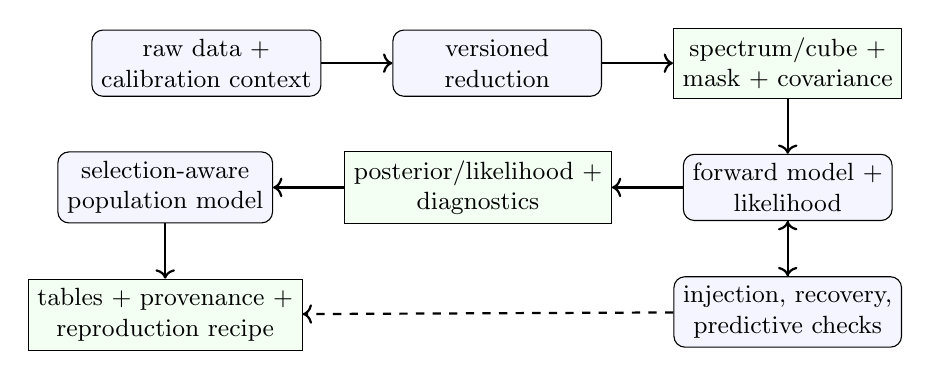
\begin{tikzpicture}[font=\small,node distance=7mm and 9mm,
stage/.style={draw,rounded corners,fill=blue!4,align=center,minimum width=2.65cm,minimum height=8mm},
artifact/.style={draw,fill=green!5,align=center,minimum width=2.65cm,minimum height=8mm},
arr/.style={->,thick}]
\node[stage] (raw) {raw data +\\calibration context};
\node[stage,right=of raw] (reduce) {versioned\\reduction};
\node[artifact,right=of reduce] (spec) {spectrum/cube +\\mask + covariance};
\node[stage,below=of spec] (fit) {forward model +\\likelihood};
\node[artifact,left=of fit] (post) {posterior/likelihood +\\diagnostics};
\node[stage,left=of post] (pop) {selection-aware\\population model};
\node[artifact,below=of pop] (release) {tables + provenance +\\reproduction recipe};
\node[stage,below=of fit] (validate) {injection, recovery,\\predictive checks};
\draw[arr] (raw)--(reduce); \draw[arr] (reduce)--(spec); \draw[arr] (spec)--(fit);
\draw[arr] (fit)--(post); \draw[arr] (post)--(pop); \draw[arr] (pop)--(release);
\draw[arr] (fit)--(validate); \draw[arr] (validate)--(fit);
\draw[arr,dashed] (validate)--(release);
\end{tikzpicture}
\caption{A reproducible line-analysis graph.  Green artifacts are preserved
interfaces; blue stages are deterministic or explicitly stochastic workflows.
Validation is part of the inference loop, not a decorative final plot.}
\label{fig:reproducible-dag}
\end{figure}

\section{Provenance and machine-readable products}

Reproducibility requires more than a code repository.  Preserve immutable raw
identifiers and checksums; calibration reference names; software and dependency
versions; configuration files; random seeds; environment or container digest;
commands; and links between inputs and outputs.  Use stable object and line IDs,
machine-readable units, explicit missing-value semantics, and documented
coordinate and time frames.  FITS remains central in astronomy, while ECSV,
ASDF, HDF5, Parquet, and domain-specific models can preserve richer structure;
the correct choice is the one accompanied by a schema and validation.
The FAIR principles - findable, accessible, interoperable, and reusable - are a
helpful publication target, but ``accessible'' need not mean unrestricted when
privacy, proprietary periods, or facility policy apply \citep{Wilkinson2016}.
Metadata and a documented route to authorized access can remain public while
controlled data stay protected.

A line catalogue should minimally carry rest wavelength or frequency with source
and medium, transition identifier, observed centroid and frame, integrated flux,
signed estimator and uncertainty, width and its definition, continuum and
equivalent width, aperture, response or resolution, covariance reference,
detection procedure, quality mask, and provenance pointer.  Store posterior
samples or a reusable likelihood for nonlinear or multimodal results when
practical.  A symmetric error bar is not an adequate serialization of a bounded,
skewed, or mixture posterior.

Continuous integration should rebuild representative reductions or synthetic
tests, validate schemas and units, verify bibliography and documentation links,
and compare scientific outputs within justified tolerances.  Exact bitwise
reproduction is desirable for deterministic stages but can be brittle across
hardware; for stochastic inference, test seeds, distributional summaries, and
coverage.  Tag the release used for a publication and archive it with a durable
identifier.  A notebook can communicate exploration, but a parameterized,
non-interactive pipeline should produce the claimed tables and figures from
declared inputs.

A robust pipeline separates pure transformations from side effects.  A command
should accept declared inputs and configuration, write outputs to a new versioned
location, and emit a manifest containing checksums and environment identity.
Workflow engines can execute a directed acyclic graph, but the graph alone is
not provenance if calibration files are downloaded by mutable URL or notebooks
depend on hidden state.  Cache keys should include scientific configuration and
reference-data versions, not only source-code commits.  Manual quality decisions
belong in append-only, machine-readable annotations with reviewer, timestamp,
reason, and supersession history.

\section{A compact analysis contract}

Before publication, write a one-page contract stating: the primary observable;
the detector-space likelihood; response and background treatment; priors and
nuisance parameters; selection function; censoring policy; atomic/model versions;
uncertainty ledger; validation tests; and exact data/code release.  This contract
does not eliminate scientific judgment.  It makes judgment visible, testable,
and replaceable - the essential properties of a durable line measurement.


\part{Reference Atlas}
\chapter{The Line-by-Line Atlas}
\label{chap:atlas}

The following reference pages are generated from the same source-cited
catalogue used by the interactive website. Wavelength convention and precision
are recorded for each entry whenever the source distinguishes air and vacuum
values.

\IfFileExists{generated/line-atlas.tex}{% Generated from data/spectral-lines.json. Do not edit.
\section{H I 21 cm}
\index{H I}

\begin{conceptbox}[At a glance]
\begin{tabularx}{\textwidth}{@{}lX@{}}
\textbf{Rest coordinate} & 1420.405751768 MHz \\
\textbf{Band} & radio / L band \\
\textbf{Transition} & 1s ground-state hyperfine F=1 -> 0 \\
\textbf{Mechanism} & magnetic-dipole hyperfine transition \\
\textbf{Primary tracers} & neutral atomic hydrogen column; gas kinematics; rotation curves; spin temperature with absorption; large-scale structure via intensity mapping \\
\textbf{Typical environments} & cold and warm neutral medium; galaxy disks; high-velocity clouds; damped Ly-alpha systems in absorption; reionization-era IGM statistically \\
\textbf{Indicative regime} & CNM roughly 20-200 K; WNM roughly 5000-10000 K; detectable outside strict LTE \\
\textbf{Density guidance} & Not a conventional density diagnostic. Emission gives optically thin H I column; emission plus absorption constrains spin temperature and covering fraction. \\
\end{tabularx}
\end{conceptbox}

H I 21 cm is produced by magnetic-dipole hyperfine transition and is encountered in cold and warm neutral medium; galaxy disks; high-velocity clouds; damped Ly-alpha systems in absorption; reionization-era IGM statistically. It is commonly used to trace neutral atomic hydrogen column; gas kinematics; rotation curves; spin temperature with absorption; large-scale structure via intensity mapping.

\subsection*{How to use it}
Use this transition with its diagnostic companions to constrain neutral atomic hydrogen column; gas kinematics; rotation curves; spin temperature with absorption; large-scale structure via intensity mapping, while fitting the continuum, line-spread function, and relevant blends.

\subsection*{Interpretive cautions}
Rest frequency is exceptionally precise. State the radio/optical/relativistic velocity convention and reference frame. Self-absorption and optical depth can hide cold gas.

\subsection*{Useful companions}
Ly-alpha 1215.6701 A; CO(1-0) 115.2712018 GHz; OH 1665/1667 MHz

\subsection*{Sources}
\texttt{NRAO\_HI\_OH; NIST\_ASD; DRAINE\_2011}

\clearpage


\section{OH 1665 MHz main line}
\index{OH}

\begin{conceptbox}[At a glance]
\begin{tabularx}{\textwidth}{@{}lX@{}}
\textbf{Rest coordinate} & 1665.4018 MHz \\
\textbf{Band} & radio / 18 cm \\
\textbf{Transition} & ground-state 2Pi3/2, J=3/2 hyperfine main-line transition \\
\textbf{Mechanism} & lambda-doubling plus hyperfine transition; often masing \\
\textbf{Primary tracers} & molecular gas magnetic field via Zeeman splitting; maser kinematics; pumped dense gas \\
\textbf{Typical environments} & massive star-forming regions; circumstellar envelopes; compact H II regions; megamaser hosts \\
\textbf{Indicative regime} & typically tens to hundreds of kelvin; non-LTE pumping controls masers \\
\textbf{Density guidance} & Population inversion depends on FIR pump, OH column and density; not a simple one-number density tracer. \\
\end{tabularx}
\end{conceptbox}

OH 1665 MHz main line is produced by lambda-doubling plus hyperfine transition; often masing and is encountered in massive star-forming regions; circumstellar envelopes; compact H II regions; megamaser hosts. It is commonly used to trace molecular gas magnetic field via Zeeman splitting; maser kinematics; pumped dense gas.

\subsection*{How to use it}
Use this transition with its diagnostic companions to constrain molecular gas magnetic field via Zeeman splitting; maser kinematics; pumped dense gas, while fitting the continuum, line-spread function, and relevant blends.

\subsection*{Interpretive cautions}
Compare 1665:1667 and satellite-line ratios to diagnose LTE departures, pumping and opacity. Strongly affected by radio-frequency interference in some bands.

\subsection*{Useful companions}
OH 1667 MHz; OH satellite lines 1612 and 1720 MHz; H2O 22 GHz maser

\subsection*{Sources}
\texttt{NRAO\_HI\_OH; JPL; SPLATALOGUE}

\clearpage


\section{OH 1667 MHz main line}
\index{OH}

\begin{conceptbox}[At a glance]
\begin{tabularx}{\textwidth}{@{}lX@{}}
\textbf{Rest coordinate} & 1667.35903 MHz \\
\textbf{Band} & radio / 18 cm \\
\textbf{Transition} & ground-state 2Pi3/2, J=3/2 hyperfine main-line transition \\
\textbf{Mechanism} & lambda-doubling plus hyperfine transition; thermal absorption/emission or maser \\
\textbf{Primary tracers} & molecular gas; dust-obscured mergers; magnetic fields; line-of-sight velocity \\
\textbf{Typical environments} & diffuse molecular clouds; star-forming regions; OH megamaser galaxies; circumstellar envelopes \\
\textbf{Indicative regime} & typically 10-300 K, with excitation set by collisions and radiative pumping \\
\textbf{Density guidance} & Line ratios are excitation/opacity diagnostics rather than direct density meters. \\
\end{tabularx}
\end{conceptbox}

OH 1667 MHz main line is produced by lambda-doubling plus hyperfine transition; thermal absorption/emission or maser and is encountered in diffuse molecular clouds; star-forming regions; OH megamaser galaxies; circumstellar envelopes. It is commonly used to trace molecular gas; dust-obscured mergers; magnetic fields; line-of-sight velocity.

\subsection*{How to use it}
Use this transition with its diagnostic companions to constrain molecular gas; dust-obscured mergers; magnetic fields; line-of-sight velocity, while fitting the continuum, line-spread function, and relevant blends.

\subsection*{Interpretive cautions}
The 1667-MHz line usually dominates extragalactic OH megamasers. Hyperfine LTE expectations can fail spectacularly under FIR pumping.

\subsection*{Useful companions}
OH 1665 MHz; OH 1612/1720 MHz; FIR OH pump transitions

\subsection*{Sources}
\texttt{NRAO\_HI\_OH; JPL; SPLATALOGUE}

\clearpage


\section{H2O 22 GHz maser}
\index{H2O}

\begin{conceptbox}[At a glance]
\begin{tabularx}{\textwidth}{@{}lX@{}}
\textbf{Rest coordinate} & 22.23508 GHz \\
\textbf{Band} & microwave / K band \\
\textbf{Transition} & 6\_16 -> 5\_23, ortho-H2O \\
\textbf{Mechanism} & collisionally pumped rotational maser \\
\textbf{Primary tracers} & sub-au kinematics; geometric distances; black-hole masses; dense shocked gas \\
\textbf{Typical environments} & shocked protostellar outflows; circumstellar envelopes; AGN accretion disks; nuclear winds \\
\textbf{Indicative regime} & commonly about 300-1000 K for strong collisional pumping \\
\textbf{Density guidance} & Maser inversion favors very dense gas, often n(H2) about 10\textasciicircum{}7-10\textasciicircum{}10 cm\textasciicircum{}-3, but geometry and velocity coherence dominate brightness. \\
\end{tabularx}
\end{conceptbox}

H2O 22 GHz maser is produced by collisionally pumped rotational maser and is encountered in shocked protostellar outflows; circumstellar envelopes; AGN accretion disks; nuclear winds. It is commonly used to trace sub-au kinematics; geometric distances; black-hole masses; dense shocked gas.

\subsection*{How to use it}
Use this transition with its diagnostic companions to constrain sub-au kinematics; geometric distances; black-hole masses; dense shocked gas, while fitting the continuum, line-spread function, and relevant blends.

\subsection*{Interpretive cautions}
Brightness temperature is non-thermal and cannot be interpreted as kinetic temperature. Narrow spikes vary and may be highly beamed.

\subsection*{Useful companions}
SiO v=1 J=1-0; OH 1665/1667 MHz; thermal sub-mm H2O lines

\subsection*{Sources}
\texttt{JPL; SPLATALOGUE; NRAO\_HI\_OH}

\clearpage


\section{NH3 (1,1) inversion}
\index{NH3}

\begin{conceptbox}[At a glance]
\begin{tabularx}{\textwidth}{@{}lX@{}}
\textbf{Rest coordinate} & 23.6944955 GHz \\
\textbf{Band} & microwave / K band \\
\textbf{Transition} & (J,K)=(1,1) inversion, resolved hyperfine complex \\
\textbf{Mechanism} & metastable inversion transition \\
\textbf{Primary tracers} & dense gas; kinetic temperature with NH3 (2,2); optical depth via satellites; velocity dispersion \\
\textbf{Typical environments} & cold dense cores; infrared dark clouds; molecular clouds; galactic nuclei \\
\textbf{Indicative regime} & especially effective near 8-40 K, but present in warmer dense gas \\
\textbf{Density guidance} & Effective excitation densities are typically around 10\textasciicircum{}3 cm\textasciicircum{}-3 and model dependent; hyperfine anomalies can affect opacity estimates. \\
\end{tabularx}
\end{conceptbox}

NH3 (1,1) inversion is produced by metastable inversion transition and is encountered in cold dense cores; infrared dark clouds; molecular clouds; galactic nuclei. It is commonly used to trace dense gas; kinetic temperature with NH3 (2,2); optical depth via satellites; velocity dispersion.

\subsection*{How to use it}
Use this transition with its diagnostic companions to constrain dense gas; kinetic temperature with NH3 (2,2); optical depth via satellites; velocity dispersion, while fitting the continuum, line-spread function, and relevant blends.

\subsection*{Interpretive cautions}
Fit the full hyperfine structure. The (2,2)/(1,1) rotational temperature is converted to kinetic temperature with a collisional model.

\subsection*{Useful companions}
NH3 (2,2) 23.7226333 GHz; NH3 (3,3) 23.8701296 GHz; N2H+ (1-0)

\subsection*{Sources}
\texttt{JPL; SPLATALOGUE; SHIRLEY\_2015}

\clearpage


\section{NH3 (2,2) inversion}
\index{NH3}

\begin{conceptbox}[At a glance]
\begin{tabularx}{\textwidth}{@{}lX@{}}
\textbf{Rest coordinate} & 23.7226333 GHz \\
\textbf{Band} & microwave / K band \\
\textbf{Transition} & (J,K)=(2,2) inversion, resolved hyperfine complex \\
\textbf{Mechanism} & metastable inversion transition \\
\textbf{Primary tracers} & gas temperature with NH3 (1,1); warmer dense component; kinematics \\
\textbf{Typical environments} & dense molecular cores; massive star-forming clumps; galactic centers \\
\textbf{Indicative regime} & roughly 15-100 K for common applications; higher metastable lines extend the thermometer \\
\textbf{Density guidance} & Similar effective-density scale to (1,1), with excitation dependent on temperature and NH3 column. \\
\end{tabularx}
\end{conceptbox}

NH3 (2,2) inversion is produced by metastable inversion transition and is encountered in dense molecular cores; massive star-forming clumps; galactic centers. It is commonly used to trace gas temperature with NH3 (1,1); warmer dense component; kinematics.

\subsection*{How to use it}
Use this transition with its diagnostic companions to constrain gas temperature with NH3 (1,1); warmer dense component; kinematics, while fitting the continuum, line-spread function, and relevant blends.

\subsection*{Interpretive cautions}
Use matched beams and simultaneous calibration when deriving temperatures; (2,2) may miss the coldest component at low signal-to-noise.

\subsection*{Useful companions}
NH3 (1,1) 23.6944955 GHz; NH3 (3,3) 23.8701296 GHz

\subsection*{Sources}
\texttt{JPL; SPLATALOGUE; SHIRLEY\_2015}

\clearpage


\section{SiO v=1 J=1-0 maser}
\index{SiO}

\begin{conceptbox}[At a glance]
\begin{tabularx}{\textwidth}{@{}lX@{}}
\textbf{Rest coordinate} & 43.122079 GHz \\
\textbf{Band} & millimetre / Q band \\
\textbf{Transition} & v=1, J=1 -> 0 \\
\textbf{Mechanism} & vibrationally excited rotational maser \\
\textbf{Primary tracers} & stellar-envelope dynamics; pulsation; magnetic-field morphology; compact shocks \\
\textbf{Typical environments} & inner envelopes of oxygen-rich AGB stars; red supergiants; rare shocked star-forming gas \\
\textbf{Indicative regime} & warm to hot molecular gas, often about 1000-2000 K near evolved stars \\
\textbf{Density guidance} & Requires high density and an inversion; representative pumping solutions use n(H2) around 10\textasciicircum{}9-10\textasciicircum{}10 cm\textasciicircum{}-3. \\
\end{tabularx}
\end{conceptbox}

SiO v=1 J=1-0 maser is produced by vibrationally excited rotational maser and is encountered in inner envelopes of oxygen-rich AGB stars; red supergiants; rare shocked star-forming gas. It is commonly used to trace stellar-envelope dynamics; pulsation; magnetic-field morphology; compact shocks.

\subsection*{How to use it}
Use this transition with its diagnostic companions to constrain stellar-envelope dynamics; pulsation; magnetic-field morphology; compact shocks, while fitting the continuum, line-spread function, and relevant blends.

\subsection*{Interpretive cautions}
Non-LTE, polarized and time variable. Do not use maser flux as a linear mass estimator.

\subsection*{Useful companions}
SiO v=2 J=1-0; SiO v=0 rotational lines; H2O 22 GHz maser

\subsection*{Sources}
\texttt{CDMS; JPL; SPLATALOGUE}

\clearpage


\section{HCN (1-0)}
\index{HCN}

\begin{conceptbox}[At a glance]
\begin{tabularx}{\textwidth}{@{}lX@{}}
\textbf{Rest coordinate} & 88.631847 GHz \\
\textbf{Band} & millimetre / 3 mm \\
\textbf{Transition} & J=1 -> 0; F=2 -> 1 strongest hyperfine component \\
\textbf{Mechanism} & electric-dipole rotational transition \\
\textbf{Primary tracers} & dense molecular gas; star-forming gas fraction; infall via self-absorption with isotopologues \\
\textbf{Typical environments} & dense molecular cores; starburst nuclei; AGN circumnuclear disks; molecular outflows \\
\textbf{Indicative regime} & commonly 10-100 K; IR pumping can matter in luminous dusty nuclei \\
\textbf{Density guidance} & Optically thin critical density is of order 10\textasciicircum{}6 cm\textasciicircum{}-3 near 10-20 K, while trapping makes effective excitation densities commonly 1-2 dex lower. \\
\end{tabularx}
\end{conceptbox}

HCN (1-0) is produced by electric-dipole rotational transition and is encountered in dense molecular cores; starburst nuclei; AGN circumnuclear disks; molecular outflows. It is commonly used to trace dense molecular gas; star-forming gas fraction; infall via self-absorption with isotopologues.

\subsection*{How to use it}
Use this transition with its diagnostic companions to constrain dense molecular gas; star-forming gas fraction; infall via self-absorption with isotopologues, while fitting the continuum, line-spread function, and relevant blends.

\subsection*{Interpretive cautions}
Resolve or model three hyperfine components in narrow Galactic sources. Opacity, abundance, electron excitation and 14-micron pumping complicate the dense-gas interpretation.

\subsection*{Useful companions}
HCO+ (1-0); HNC (1-0); H13CN (1-0); CN (1-0)

\subsection*{Sources}
\texttt{CDMS; SPLATALOGUE; SHIRLEY\_2015}

\clearpage


\section{HCO+ (1-0)}
\index{HCO+}

\begin{conceptbox}[At a glance]
\begin{tabularx}{\textwidth}{@{}lX@{}}
\textbf{Rest coordinate} & 89.188526 GHz \\
\textbf{Band} & millimetre / 3 mm \\
\textbf{Transition} & J=1 -> 0 \\
\textbf{Mechanism} & electric-dipole rotational transition of a molecular ion \\
\textbf{Primary tracers} & dense ionized-molecular chemistry; infall/outflow profiles; cosmic-ray ionization indirectly \\
\textbf{Typical environments} & dense molecular clouds; protostellar envelopes; galaxy nuclei; outflows \\
\textbf{Indicative regime} & about 10-100 K in most applications \\
\textbf{Density guidance} & Critical density is a few 10\textasciicircum{}5 cm\textasciicircum{}-3, but effective excitation density can be around 10\textasciicircum{}3-10\textasciicircum{}4 cm\textasciicircum{}-3 depending on opacity and column. \\
\end{tabularx}
\end{conceptbox}

HCO+ (1-0) is produced by electric-dipole rotational transition of a molecular ion and is encountered in dense molecular clouds; protostellar envelopes; galaxy nuclei; outflows. It is commonly used to trace dense ionized-molecular chemistry; infall/outflow profiles; cosmic-ray ionization indirectly.

\subsection*{How to use it}
Use this transition with its diagnostic companions to constrain dense ionized-molecular chemistry; infall/outflow profiles; cosmic-ray ionization indirectly, while fitting the continuum, line-spread function, and relevant blends.

\subsection*{Interpretive cautions}
Often optically thick and self-absorbed. Pair with H13CO+ to estimate opacity; abundance is sensitive to ionization and water/CO chemistry.

\subsection*{Useful companions}
HCN (1-0); H13CO+ (1-0); CO isotopologues; N2H+ (1-0)

\subsection*{Sources}
\texttt{CDMS; SPLATALOGUE; SHIRLEY\_2015}

\clearpage


\section{N2H+ (1-0)}
\index{N2H+}

\begin{conceptbox}[At a glance]
\begin{tabularx}{\textwidth}{@{}lX@{}}
\textbf{Rest coordinate} & 93.173764 GHz \\
\textbf{Band} & millimetre / 3 mm \\
\textbf{Transition} & J=1 -> 0 hyperfine multiplet \\
\textbf{Mechanism} & electric-dipole rotational transition with nitrogen hyperfine structure \\
\textbf{Primary tracers} & cold dense gas; systemic velocity; optical depth from hyperfine fitting; CO freeze-out zones \\
\textbf{Typical environments} & cold prestellar cores; dense filaments; protostellar envelopes; CO-depleted gas \\
\textbf{Indicative regime} & especially useful around 7-30 K \\
\textbf{Density guidance} & Critical density is roughly 10\textasciicircum{}5 cm\textasciicircum{}-3; radiative trapping and hyperfine excitation lower the effective threshold. \\
\end{tabularx}
\end{conceptbox}

N2H+ (1-0) is produced by electric-dipole rotational transition with nitrogen hyperfine structure and is encountered in cold prestellar cores; dense filaments; protostellar envelopes; CO-depleted gas. It is commonly used to trace cold dense gas; systemic velocity; optical depth from hyperfine fitting; CO freeze-out zones.

\subsection*{How to use it}
Use this transition with its diagnostic companions to constrain cold dense gas; systemic velocity; optical depth from hyperfine fitting; CO freeze-out zones, while fitting the continuum, line-spread function, and relevant blends.

\subsection*{Interpretive cautions}
The quoted value is a conventional reference for the hyperfine complex; precision velocity work must adopt component-specific frequencies and a consistent catalog.

\subsection*{Useful companions}
NH3 (1,1); HCO+ (1-0); C18O (1-0); N2D+

\subsection*{Sources}
\texttt{CDMS; SPLATALOGUE; SHIRLEY\_2015}

\clearpage


\section{CS (2-1)}
\index{CS}

\begin{conceptbox}[At a glance]
\begin{tabularx}{\textwidth}{@{}lX@{}}
\textbf{Rest coordinate} & 97.980953 GHz \\
\textbf{Band} & millimetre / 3 mm \\
\textbf{Transition} & J=2 -> 1 \\
\textbf{Mechanism} & electric-dipole rotational transition \\
\textbf{Primary tracers} & dense gas; velocity structure; sulfur chemistry \\
\textbf{Typical environments} & dense clumps; massive star-forming regions; galactic centers; shocked molecular gas \\
\textbf{Indicative regime} & about 10-100 K \\
\textbf{Density guidance} & Critical density is a few 10\textasciicircum{}5 cm\textasciicircum{}-3, with a substantially lower effective excitation density for optically thick bright columns. \\
\end{tabularx}
\end{conceptbox}

CS (2-1) is produced by electric-dipole rotational transition and is encountered in dense clumps; massive star-forming regions; galactic centers; shocked molecular gas. It is commonly used to trace dense gas; velocity structure; sulfur chemistry.

\subsection*{How to use it}
Use this transition with its diagnostic companions to constrain dense gas; velocity structure; sulfur chemistry, while fitting the continuum, line-spread function, and relevant blends.

\subsection*{Interpretive cautions}
CS can deplete in cold cores and become optically thick; use isotopologues and multi-J excitation rather than a single conversion factor.

\subsection*{Useful companions}
C34S (2-1); HCN (1-0); CS higher-J ladder

\subsection*{Sources}
\texttt{CDMS; JPL; SHIRLEY\_2015}

\clearpage


\section{C18O (1-0)}
\index{C18O}

\begin{conceptbox}[At a glance]
\begin{tabularx}{\textwidth}{@{}lX@{}}
\textbf{Rest coordinate} & 109.7821734 GHz \\
\textbf{Band} & millimetre / 3 mm \\
\textbf{Transition} & J=1 -> 0 \\
\textbf{Mechanism} & electric-dipole rotational transition \\
\textbf{Primary tracers} & moderate-column molecular gas; CO optical-depth correction; gas kinematics \\
\textbf{Typical environments} & molecular clouds; dense cores; protoplanetary disks; galaxy molecular disks \\
\textbf{Indicative regime} & cold molecular gas, commonly 8-50 K \\
\textbf{Density guidance} & Critical density is around 10\textasciicircum{}3 cm\textasciicircum{}-3 and effective excitation density lower; abundance and shielding often dominate detectability. \\
\end{tabularx}
\end{conceptbox}

C18O (1-0) is produced by electric-dipole rotational transition and is encountered in molecular clouds; dense cores; protoplanetary disks; galaxy molecular disks. It is commonly used to trace moderate-column molecular gas; CO optical-depth correction; gas kinematics.

\subsection*{How to use it}
Use this transition with its diagnostic companions to constrain moderate-column molecular gas; CO optical-depth correction; gas kinematics, while fitting the continuum, line-spread function, and relevant blends.

\subsection*{Interpretive cautions}
Usually thinner than 13CO but not guaranteed optically thin. Selective photodissociation, fractionation and isotope-ratio gradients bias mass estimates.

\subsection*{Useful companions}
13CO (1-0); 12CO (1-0); C17O (1-0); dust continuum

\subsection*{Sources}
\texttt{CDMS; JPL; CARILLI\_WALTER\_2013}

\clearpage


\section{13CO (1-0)}
\index{13CO}

\begin{conceptbox}[At a glance]
\begin{tabularx}{\textwidth}{@{}lX@{}}
\textbf{Rest coordinate} & 110.2013543 GHz \\
\textbf{Band} & millimetre / 3 mm \\
\textbf{Transition} & J=1 -> 0 \\
\textbf{Mechanism} & electric-dipole rotational transition \\
\textbf{Primary tracers} & molecular column; 12CO opacity; cloud structure; isotope chemistry \\
\textbf{Typical environments} & molecular clouds; galaxy disks; circumstellar envelopes; protoplanetary disks \\
\textbf{Indicative regime} & commonly 8-100 K \\
\textbf{Density guidance} & Critical density is around 10\textasciicircum{}3 cm\textasciicircum{}-3; photon trapping lowers the effective excitation threshold. \\
\end{tabularx}
\end{conceptbox}

13CO (1-0) is produced by electric-dipole rotational transition and is encountered in molecular clouds; galaxy disks; circumstellar envelopes; protoplanetary disks. It is commonly used to trace molecular column; 12CO opacity; cloud structure; isotope chemistry.

\subsection*{How to use it}
Use this transition with its diagnostic companions to constrain molecular column; 12CO opacity; cloud structure; isotope chemistry, while fitting the continuum, line-spread function, and relevant blends.

\subsection*{Interpretive cautions}
Often optically thick in cloud peaks. Carbon isotope gradients, chemical fractionation and selective photodissociation prevent a universal 12CO/13CO abundance ratio.

\subsection*{Useful companions}
12CO (1-0); C18O (1-0); 13CO higher-J lines

\subsection*{Sources}
\texttt{CDMS; JPL; CARILLI\_WALTER\_2013}

\clearpage


\section{12CO (1-0)}
\index{12CO}

\begin{conceptbox}[At a glance]
\begin{tabularx}{\textwidth}{@{}lX@{}}
\textbf{Rest coordinate} & 115.2712018 GHz \\
\textbf{Band} & millimetre / 2.6 mm \\
\textbf{Transition} & J=1 -> 0 \\
\textbf{Mechanism} & electric-dipole rotational transition \\
\textbf{Primary tracers} & bulk molecular gas via CO-to-H2 conversion; kinematics; cloud temperature when thick \\
\textbf{Typical environments} & molecular clouds; galaxy disks; starbursts; circumstellar envelopes; molecular outflows \\
\textbf{Indicative regime} & cold molecular gas from about 5 K upward; upper-state energy is 5.53 K \\
\textbf{Density guidance} & Optically thin critical density is roughly 2x10\textasciicircum{}3 cm\textasciicircum{}-3, while trapping permits bright emission at a few 10\textasciicircum{}2 cm\textasciicircum{}-3 or below. \\
\end{tabularx}
\end{conceptbox}

12CO (1-0) is produced by electric-dipole rotational transition and is encountered in molecular clouds; galaxy disks; starbursts; circumstellar envelopes; molecular outflows. It is commonly used to trace bulk molecular gas via CO-to-H2 conversion; kinematics; cloud temperature when thick.

\subsection*{How to use it}
Use this transition with its diagnostic companions to constrain bulk molecular gas via CO-to-H2 conversion; kinematics; cloud temperature when thick, while fitting the continuum, line-spread function, and relevant blends.

\subsection*{Interpretive cautions}
Usually optically thick. X\_CO depends on metallicity, dynamics, excitation, spatial scale and radiation field; CMB contrast matters at high redshift.

\subsection*{Useful companions}
13CO (1-0); C18O (1-0); CO (2-1); dust continuum

\subsection*{Sources}
\texttt{CDMS; JPL; CARILLI\_WALTER\_2013}

\clearpage


\section{12CO (2-1)}
\index{12CO}

\begin{conceptbox}[At a glance]
\begin{tabularx}{\textwidth}{@{}lX@{}}
\textbf{Rest coordinate} & 230.538 GHz \\
\textbf{Band} & submillimetre / 1.3 mm \\
\textbf{Transition} & J=2 -> 1 \\
\textbf{Mechanism} & electric-dipole rotational transition \\
\textbf{Primary tracers} & molecular gas distribution; excitation with CO(1-0); kinematics \\
\textbf{Typical environments} & molecular clouds; nearby and high-redshift galaxies; disks; outflows \\
\textbf{Indicative regime} & cold to moderately warm gas; upper-state energy is 16.6 K \\
\textbf{Density guidance} & Critical density is around 10\textasciicircum{}4 cm\textasciicircum{}-3, but opacity makes the effective density much lower. \\
\end{tabularx}
\end{conceptbox}

12CO (2-1) is produced by electric-dipole rotational transition and is encountered in molecular clouds; nearby and high-redshift galaxies; disks; outflows. It is commonly used to trace molecular gas distribution; excitation with CO(1-0); kinematics.

\subsection*{How to use it}
Use this transition with its diagnostic companions to constrain molecular gas distribution; excitation with CO(1-0); kinematics, while fitting the continuum, line-spread function, and relevant blends.

\subsection*{Interpretive cautions}
Brightness-temperature ratio r21 is sensitive to excitation, beam filling and optical depth. Match angular resolution before interpreting line ratios.

\subsection*{Useful companions}
CO (1-0); CO (3-2); 13CO (2-1)

\subsection*{Sources}
\texttt{CDMS; JPL; CARILLI\_WALTER\_2013}

\clearpage


\section{12CO (3-2)}
\index{12CO}

\begin{conceptbox}[At a glance]
\begin{tabularx}{\textwidth}{@{}lX@{}}
\textbf{Rest coordinate} & 345.7959899 GHz \\
\textbf{Band} & submillimetre / 870 micron \\
\textbf{Transition} & J=3 -> 2 \\
\textbf{Mechanism} & electric-dipole rotational transition \\
\textbf{Primary tracers} & warmer/denser molecular component; CO excitation ladder; kinematics \\
\textbf{Typical environments} & warm molecular clouds; star-forming clumps; starbursts; high-redshift galaxies \\
\textbf{Indicative regime} & commonly 20-100 K; upper-state energy is 33.2 K \\
\textbf{Density guidance} & Critical density is a few 10\textasciicircum{}4 cm\textasciicircum{}-3; radiative trapping lowers the effective density. \\
\end{tabularx}
\end{conceptbox}

12CO (3-2) is produced by electric-dipole rotational transition and is encountered in warm molecular clouds; star-forming clumps; starbursts; high-redshift galaxies. It is commonly used to trace warmer/denser molecular component; CO excitation ladder; kinematics.

\subsection*{How to use it}
Use this transition with its diagnostic companions to constrain warmer/denser molecular component; CO excitation ladder; kinematics, while fitting the continuum, line-spread function, and relevant blends.

\subsection*{Interpretive cautions}
Mid-J selection can bias samples toward excited gas. Use a CO SLED and consistent beam/uv coverage to infer multiple gas phases.

\subsection*{Useful companions}
CO (2-1); CO (4-3); 13CO (3-2); [C I] 492 GHz

\subsection*{Sources}
\texttt{CDMS; JPL; CARILLI\_WALTER\_2013}

\clearpage


\section{[C I] 609 micron}
\index{C I}

\begin{conceptbox}[At a glance]
\begin{tabularx}{\textwidth}{@{}lX@{}}
\textbf{Rest coordinate} & 492.160651 GHz \\
\textbf{Band} & submillimetre / far-infrared \\
\textbf{Transition} & 3P1 -> 3P0 \\
\textbf{Mechanism} & magnetic-dipole fine-structure transition \\
\textbf{Primary tracers} & neutral carbon mass; molecular gas when calibrated; excitation with [C I](2-1) \\
\textbf{Typical environments} & molecular clouds; PDRs; high-redshift galaxies; CO-dark molecular interfaces \\
\textbf{Indicative regime} & cold molecular gas, commonly 15-60 K; upper level is 23.6 K above ground \\
\textbf{Density guidance} & Critical density with H2 is of order 5x10\textasciicircum{}2 cm\textasciicircum{}-3, weakly model dependent. \\
\end{tabularx}
\end{conceptbox}

[C I] 609 micron is produced by magnetic-dipole fine-structure transition and is encountered in molecular clouds; PDRs; high-redshift galaxies; CO-dark molecular interfaces. It is commonly used to trace neutral carbon mass; molecular gas when calibrated; excitation with [C I](2-1).

\subsection*{How to use it}
Use this transition with its diagnostic companions to constrain neutral carbon mass; molecular gas when calibrated; excitation with [C I](2-1), while fitting the continuum, line-spread function, and relevant blends.

\subsection*{Interpretive cautions}
The two [C I] lines give an excitation temperature only under a common, often optically thin one-zone assumption. Carbon abundance is not universal.

\subsection*{Useful companions}
[C I] 809 GHz; CO rotational ladder; [C II] 158 micron

\subsection*{Sources}
\texttt{NIST\_ASD; CDMS; CARILLI\_WALTER\_2013}

\clearpage


\section{[C I] 370 micron}
\index{C I}

\begin{conceptbox}[At a glance]
\begin{tabularx}{\textwidth}{@{}lX@{}}
\textbf{Rest coordinate} & 809.34197 GHz \\
\textbf{Band} & submillimetre / far-infrared \\
\textbf{Transition} & 3P2 -> 3P1 \\
\textbf{Mechanism} & magnetic-dipole fine-structure transition \\
\textbf{Primary tracers} & neutral carbon excitation; molecular gas temperature; carbon mass \\
\textbf{Typical environments} & warm molecular clouds; PDRs; starbursts; high-redshift galaxies \\
\textbf{Indicative regime} & typically 25-100 K; upper level is 62.5 K above ground \\
\textbf{Density guidance} & Critical density with H2 is of order 10\textasciicircum{}3 cm\textasciicircum{}-3. \\
\end{tabularx}
\end{conceptbox}

[C I] 370 micron is produced by magnetic-dipole fine-structure transition and is encountered in warm molecular clouds; PDRs; starbursts; high-redshift galaxies. It is commonly used to trace neutral carbon excitation; molecular gas temperature; carbon mass.

\subsection*{How to use it}
Use this transition with its diagnostic companions to constrain neutral carbon excitation; molecular gas temperature; carbon mass, while fitting the continuum, line-spread function, and relevant blends.

\subsection*{Interpretive cautions}
The line sits close to CO(7-6) in frequency, useful for simultaneous setups but demanding correct identification at uncertain redshift.

\subsection*{Useful companions}
[C I] 492 GHz; CO (7-6) nearby in frequency; [C II] 158 micron

\subsection*{Sources}
\texttt{NIST\_ASD; CDMS; CARILLI\_WALTER\_2013}

\clearpage


\section{[C II] 158 micron}
\index{C II}

\begin{conceptbox}[At a glance]
\begin{tabularx}{\textwidth}{@{}lX@{}}
\textbf{Rest coordinate} & 1900.5369 GHz \\
\textbf{Band} & far-infrared \\
\textbf{Transition} & 2P3/2 -> 2P1/2 \\
\textbf{Mechanism} & fine-structure transition \\
\textbf{Primary tracers} & gas cooling; star-forming ISM; dynamics and redshift; CO-dark molecular gas with modeling \\
\textbf{Typical environments} & PDR surfaces; diffuse neutral gas; CO-dark H2; diffuse ionized gas; high-redshift galaxies \\
\textbf{Indicative regime} & upper level corresponds to 91.2 K; excited in neutral and ionized gas from roughly 50 K to 10\textasciicircum{}4 K \\
\textbf{Density guidance} & Approximate critical densities: about 50 cm\textasciicircum{}-3 for electrons, 3x10\textasciicircum{}3 for H and 5x10\textasciicircum{}3 for H2, with temperature dependence. \\
\end{tabularx}
\end{conceptbox}

[C II] 158 micron is produced by fine-structure transition and is encountered in PDR surfaces; diffuse neutral gas; CO-dark H2; diffuse ionized gas; high-redshift galaxies. It is commonly used to trace gas cooling; star-forming ISM; dynamics and redshift; CO-dark molecular gas with modeling.

\subsection*{How to use it}
Use this transition with its diagnostic companions to constrain gas cooling; star-forming ISM; dynamics and redshift; CO-dark molecular gas with modeling, while fitting the continuum, line-spread function, and relevant blends.

\subsection*{Interpretive cautions}
A multiphase line, not a pure PDR or SFR tracer. Optical depth, foreground absorption and the high-surface-brightness [C II] deficit affect interpretation.

\subsection*{Useful companions}
[N II] 205 micron to isolate ionized contribution; [O I] 63 micron; CO rotational lines; FIR continuum

\subsection*{Sources}
\texttt{NIST\_ASD; CARILLI\_WALTER\_2013; HOLLENBACH\_TIELENS\_1999}

\clearpage


\section{[N II] 205 micron}
\index{N II}

\begin{conceptbox}[At a glance]
\begin{tabularx}{\textwidth}{@{}lX@{}}
\textbf{Rest coordinate} & 1461.1319 GHz \\
\textbf{Band} & far-infrared \\
\textbf{Transition} & 3P1 -> 3P0 \\
\textbf{Mechanism} & fine-structure transition \\
\textbf{Primary tracers} & ionized-gas mass; massive-star ionization; ionized contribution to [C II] \\
\textbf{Typical environments} & diffuse ionized medium; H II regions; star-forming galaxies \\
\textbf{Indicative regime} & ionized gas near 6000-10000 K; excitation energy is only about 70 K \\
\textbf{Density guidance} & Electron critical density is roughly 40-50 cm\textasciicircum{}-3; the 122/205 ratio measures electron density over roughly 1-10\textasciicircum{}3 cm\textasciicircum{}-3. \\
\end{tabularx}
\end{conceptbox}

[N II] 205 micron is produced by fine-structure transition and is encountered in diffuse ionized medium; H II regions; star-forming galaxies. It is commonly used to trace ionized-gas mass; massive-star ionization; ionized contribution to [C II].

\subsection*{How to use it}
Use this transition with its diagnostic companions to constrain ionized-gas mass; massive-star ionization; ionized contribution to [C II], while fitting the continuum, line-spread function, and relevant blends.

\subsection*{Interpretive cautions}
N+ requires ionized gas because its formation threshold exceeds 13.6 eV. Low critical density makes 205 micron particularly sensitive to diffuse ionized material.

\subsection*{Useful companions}
[N II] 122 micron; [C II] 158 micron; radio free-free emission

\subsection*{Sources}
\texttt{NIST\_NII; CARILLI\_WALTER\_2013; OSTERBROCK\_FERLAND\_2006}

\clearpage


\section{[N II] 122 micron}
\index{N II}

\begin{conceptbox}[At a glance]
\begin{tabularx}{\textwidth}{@{}lX@{}}
\textbf{Rest coordinate} & 2459.38006 GHz \\
\textbf{Band} & far-infrared \\
\textbf{Transition} & 3P2 -> 3P1 \\
\textbf{Mechanism} & fine-structure transition \\
\textbf{Primary tracers} & electron density with 205 micron; ionized-gas cooling; massive-star photoionization \\
\textbf{Typical environments} & H II regions; diffuse ionized gas; star-forming galaxies \\
\textbf{Indicative regime} & ionized gas around 6000-10000 K \\
\textbf{Density guidance} & Electron critical density is about 300 cm\textasciicircum{}-3; 122/205 is a robust density ratio when both lines sample the same gas. \\
\end{tabularx}
\end{conceptbox}

[N II] 122 micron is produced by fine-structure transition and is encountered in H II regions; diffuse ionized gas; star-forming galaxies. It is commonly used to trace electron density with 205 micron; ionized-gas cooling; massive-star photoionization.

\subsection*{How to use it}
Use this transition with its diagnostic companions to constrain electron density with 205 micron; ionized-gas cooling; massive-star photoionization, while fitting the continuum, line-spread function, and relevant blends.

\subsection*{Interpretive cautions}
Far-IR dust extinction is small, but aperture mismatch and multi-density structure can bias the ratio.

\subsection*{Useful companions}
[N II] 205 micron; [O III] 88 micron; [C II] 158 micron

\subsection*{Sources}
\texttt{NIST\_NII; CARILLI\_WALTER\_2013; OSTERBROCK\_FERLAND\_2006}

\clearpage


\section{[O I] 145 micron}
\index{O I}

\begin{conceptbox}[At a glance]
\begin{tabularx}{\textwidth}{@{}lX@{}}
\textbf{Rest coordinate} & 145.525 micron \\
\textbf{Band} & far-infrared \\
\textbf{Transition} & 3P0 -> 3P1 \\
\textbf{Mechanism} & fine-structure transition \\
\textbf{Primary tracers} & neutral-gas cooling; PDR density and radiation field with [O I] 63/[C II]; shock-heated gas \\
\textbf{Typical environments} & warm dense PDRs; shocks; neutral gas near H II regions \\
\textbf{Indicative regime} & warm neutral gas, commonly about 100-1000 K \\
\textbf{Density guidance} & Critical density for H/H2 collisions is of order 10\textasciicircum{}5 cm\textasciicircum{}-3, model dependent. \\
\end{tabularx}
\end{conceptbox}

[O I] 145 micron is produced by fine-structure transition and is encountered in warm dense PDRs; shocks; neutral gas near H II regions. It is commonly used to trace neutral-gas cooling; PDR density and radiation field with [O I] 63/[C II]; shock-heated gas.

\subsection*{How to use it}
Use this transition with its diagnostic companions to constrain neutral-gas cooling; PDR density and radiation field with [O I] 63/[C II]; shock-heated gas, while fitting the continuum, line-spread function, and relevant blends.

\subsection*{Interpretive cautions}
Usually weaker but less self-absorbed than the 63-micron line. The 63/145 ratio can reveal opacity, foreground absorption, temperature and density.

\subsection*{Useful companions}
[O I] 63 micron; [C II] 158 micron; high-J CO

\subsection*{Sources}
\texttt{NIST\_ASD; HOLLENBACH\_TIELENS\_1999; CARILLI\_WALTER\_2013}

\clearpage


\section{[O I] 63 micron}
\index{O I}

\begin{conceptbox}[At a glance]
\begin{tabularx}{\textwidth}{@{}lX@{}}
\textbf{Rest coordinate} & 63.1837 micron \\
\textbf{Band} & far-infrared \\
\textbf{Transition} & 3P1 -> 3P2 \\
\textbf{Mechanism} & fine-structure transition \\
\textbf{Primary tracers} & dominant neutral-gas cooling in warm dense regions; FUV field; shock power \\
\textbf{Typical environments} & dense warm PDRs; dissociative and non-dissociative shocks; protostellar outflows \\
\textbf{Indicative regime} & upper level is about 228 K; strongest in gas roughly 100-1000 K \\
\textbf{Density guidance} & Critical density for collisions with H is roughly 5x10\textasciicircum{}5 cm\textasciicircum{}-3; optical depth often matters first. \\
\end{tabularx}
\end{conceptbox}

[O I] 63 micron is produced by fine-structure transition and is encountered in dense warm PDRs; dissociative and non-dissociative shocks; protostellar outflows. It is commonly used to trace dominant neutral-gas cooling in warm dense regions; FUV field; shock power.

\subsection*{How to use it}
Use this transition with its diagnostic companions to constrain dominant neutral-gas cooling in warm dense regions; FUV field; shock power, while fitting the continuum, line-spread function, and relevant blends.

\subsection*{Interpretive cautions}
Can be optically thick and self-absorbed by colder foreground O I; a line deficit does not uniquely imply weak PDR heating.

\subsection*{Useful companions}
[O I] 145 micron; [C II] 158 micron; H2 rotational lines

\subsection*{Sources}
\texttt{NIST\_ASD; HOLLENBACH\_TIELENS\_1999; CARILLI\_WALTER\_2013}

\clearpage


\section{[O III] 88 micron}
\index{O III}

\begin{conceptbox}[At a glance]
\begin{tabularx}{\textwidth}{@{}lX@{}}
\textbf{Rest coordinate} & 3393.006 GHz \\
\textbf{Band} & far-infrared \\
\textbf{Transition} & 3P1 -> 3P0 \\
\textbf{Mechanism} & fine-structure transition \\
\textbf{Primary tracers} & hard massive-star radiation; ionized gas; electron density with 52 micron; high-redshift systemic redshift \\
\textbf{Typical environments} & H II regions; low-metallicity star-forming galaxies; planetary nebulae; reionization-era galaxies \\
\textbf{Indicative regime} & photoionized gas around 7000-20000 K; low excitation energy minimizes temperature sensitivity \\
\textbf{Density guidance} & Electron critical density is about 500 cm\textasciicircum{}-3; 52/88 measures densities from roughly 10\textasciicircum{}2 to 10\textasciicircum{}4 cm\textasciicircum{}-3. \\
\end{tabularx}
\end{conceptbox}

[O III] 88 micron is produced by fine-structure transition and is encountered in H II regions; low-metallicity star-forming galaxies; planetary nebulae; reionization-era galaxies. It is commonly used to trace hard massive-star radiation; ionized gas; electron density with 52 micron; high-redshift systemic redshift.

\subsection*{How to use it}
Use this transition with its diagnostic companions to constrain hard massive-star radiation; ionized gas; electron density with 52 micron; high-redshift systemic redshift, while fitting the continuum, line-spread function, and relevant blends.

\subsection*{Interpretive cautions}
Bright in hard, low-metallicity H II regions and relatively extinction-free. Abundance, ionization parameter and density all affect line-to-SFR conversions.

\subsection*{Useful companions}
[O III] 52 micron; [N II] 122 micron; optical [O III] 5008 A

\subsection*{Sources}
\texttt{NIST\_ASD; CARILLI\_WALTER\_2013; OSTERBROCK\_FERLAND\_2006}

\clearpage


\section{[O III] 52 micron}
\index{O III}

\begin{conceptbox}[At a glance]
\begin{tabularx}{\textwidth}{@{}lX@{}}
\textbf{Rest coordinate} & 51.8145 micron \\
\textbf{Band} & far-infrared \\
\textbf{Transition} & 3P2 -> 3P1 \\
\textbf{Mechanism} & fine-structure transition \\
\textbf{Primary tracers} & electron density with 88 micron; hard ionizing field; ionized-gas cooling \\
\textbf{Typical environments} & compact H II regions; planetary nebulae; starbursts \\
\textbf{Indicative regime} & photoionized gas around 7000-20000 K \\
\textbf{Density guidance} & Electron critical density is roughly 3.6x10\textasciicircum{}3 cm\textasciicircum{}-3; 52/88 is a standard far-IR density diagnostic. \\
\end{tabularx}
\end{conceptbox}

[O III] 52 micron is produced by fine-structure transition and is encountered in compact H II regions; planetary nebulae; starbursts. It is commonly used to trace electron density with 88 micron; hard ionizing field; ionized-gas cooling.

\subsection*{How to use it}
Use this transition with its diagnostic companions to constrain electron density with 88 micron; hard ionizing field; ionized-gas cooling, while fitting the continuum, line-spread function, and relevant blends.

\subsection*{Interpretive cautions}
Use matched apertures. At high density both lines approach LTE and the ratio saturates; abundance and ionization structure remain separate uncertainties.

\subsection*{Useful companions}
[O III] 88 micron; optical [O III] 5008 A; [N III] 57 micron

\subsection*{Sources}
\texttt{MPE\_FINE\_STRUCTURE; CARILLI\_WALTER\_2013; OSTERBROCK\_FERLAND\_2006}

\clearpage


\section{[Si II] 34.8 micron}
\index{Si II}

\begin{conceptbox}[At a glance]
\begin{tabularx}{\textwidth}{@{}lX@{}}
\textbf{Rest coordinate} & 34.814 micron \\
\textbf{Band} & mid-infrared \\
\textbf{Transition} & 2P3/2 -> 2P1/2 \\
\textbf{Mechanism} & fine-structure transition \\
\textbf{Primary tracers} & gas cooling; silicon released from grains; PDR/XDR/shock conditions \\
\textbf{Typical environments} & PDRs; diffuse ionized gas; shocks; X-ray-dominated regions \\
\textbf{Indicative regime} & warm neutral or ionized gas, about 100-10000 K \\
\textbf{Density guidance} & Critical density is roughly 10\textasciicircum{}3 cm\textasciicircum{}-3 for electrons and a few 10\textasciicircum{}5 cm\textasciicircum{}-3 for H, with temperature dependence. \\
\end{tabularx}
\end{conceptbox}

[Si II] 34.8 micron is produced by fine-structure transition and is encountered in PDRs; diffuse ionized gas; shocks; X-ray-dominated regions. It is commonly used to trace gas cooling; silicon released from grains; PDR/XDR/shock conditions.

\subsection*{How to use it}
Use this transition with its diagnostic companions to constrain gas cooling; silicon released from grains; PDR/XDR/shock conditions, while fitting the continuum, line-spread function, and relevant blends.

\subsection*{Interpretive cautions}
Silicon depletion and grain destruction dominate absolute calibration; strong emission may arise from multiple phases along the same sightline.

\subsection*{Useful companions}
[Fe II] 26 micron; [S III] 33.5 micron; [C II] 158 micron

\subsection*{Sources}
\texttt{ISO\_SWS; MPE\_FINE\_STRUCTURE; HOLLENBACH\_TIELENS\_1999}

\clearpage


\section{[S III] 33.5 micron}
\index{S III}

\begin{conceptbox}[At a glance]
\begin{tabularx}{\textwidth}{@{}lX@{}}
\textbf{Rest coordinate} & 33.481 micron \\
\textbf{Band} & mid-infrared \\
\textbf{Transition} & 3P1 -> 3P0 \\
\textbf{Mechanism} & fine-structure transition \\
\textbf{Primary tracers} & ionized gas; electron density with 18.7 micron; sulfur abundance with modeling \\
\textbf{Typical environments} & H II regions; starburst galaxies; planetary nebulae \\
\textbf{Indicative regime} & photoionized gas around 5000-15000 K \\
\textbf{Density guidance} & Electron critical density is of order 10\textasciicircum{}3 cm\textasciicircum{}-3; the 18.7/33.5 ratio spans roughly 10\textasciicircum{}2-10\textasciicircum{}4 cm\textasciicircum{}-3. \\
\end{tabularx}
\end{conceptbox}

[S III] 33.5 micron is produced by fine-structure transition and is encountered in H II regions; starburst galaxies; planetary nebulae. It is commonly used to trace ionized gas; electron density with 18.7 micron; sulfur abundance with modeling.

\subsection*{How to use it}
Use this transition with its diagnostic companions to constrain ionized gas; electron density with 18.7 micron; sulfur abundance with modeling, while fitting the continuum, line-spread function, and relevant blends.

\subsection*{Interpretive cautions}
The widely separated pair is susceptible to aperture and extinction mismatch; use the correct low-density limit for the adopted atomic data.

\subsection*{Useful companions}
[S III] 18.7 micron; optical [S III] 9071/9533 A; [Ne II] 12.8 micron

\subsection*{Sources}
\texttt{ISO\_SWS; MPE\_FINE\_STRUCTURE; OSTERBROCK\_FERLAND\_2006}

\clearpage


\section{[S III] 18.7 micron}
\index{S III}

\begin{conceptbox}[At a glance]
\begin{tabularx}{\textwidth}{@{}lX@{}}
\textbf{Rest coordinate} & 18.713 micron \\
\textbf{Band} & mid-infrared \\
\textbf{Transition} & 3P2 -> 3P1 \\
\textbf{Mechanism} & fine-structure transition \\
\textbf{Primary tracers} & electron density with 33.5 micron; ionized gas; obscured star formation \\
\textbf{Typical environments} & H II regions; compact starbursts; planetary nebulae \\
\textbf{Indicative regime} & photoionized gas around 5000-15000 K \\
\textbf{Density guidance} & Electron critical density is roughly 2x10\textasciicircum{}4 cm\textasciicircum{}-3; 18.7/33.5 rises with density before saturating. \\
\end{tabularx}
\end{conceptbox}

[S III] 18.7 micron is produced by fine-structure transition and is encountered in H II regions; compact starbursts; planetary nebulae. It is commonly used to trace electron density with 33.5 micron; ionized gas; obscured star formation.

\subsection*{How to use it}
Use this transition with its diagnostic companions to constrain electron density with 33.5 micron; ionized gas; obscured star formation, while fitting the continuum, line-spread function, and relevant blends.

\subsection*{Interpretive cautions}
Less affected by dust than optical lines but can suffer silicate-feature continuum systematics and aperture differences.

\subsection*{Useful companions}
[S III] 33.5 micron; [Ne III] 15.6 micron; optical [S II] density pair

\subsection*{Sources}
\texttt{ISO\_SWS; MPE\_FINE\_STRUCTURE; OSTERBROCK\_FERLAND\_2006}

\clearpage


\section{[Ne II] 12.8 micron}
\index{Ne II}

\begin{conceptbox}[At a glance]
\begin{tabularx}{\textwidth}{@{}lX@{}}
\textbf{Rest coordinate} & 12.814 micron \\
\textbf{Band} & mid-infrared \\
\textbf{Transition} & 2P1/2 -> 2P3/2 \\
\textbf{Mechanism} & fine-structure transition \\
\textbf{Primary tracers} & obscured massive-star ionization; ionized-gas kinematics; soft-to-moderate radiation fields \\
\textbf{Typical environments} & H II regions; embedded star formation; protoplanetary disk surfaces; AGN narrow-line regions \\
\textbf{Indicative regime} & photoionized gas around 5000-15000 K \\
\textbf{Density guidance} & Electron critical density is of order 6x10\textasciicircum{}5 cm\textasciicircum{}-3; usually in the low-density limit for extended H II gas. \\
\end{tabularx}
\end{conceptbox}

[Ne II] 12.8 micron is produced by fine-structure transition and is encountered in H II regions; embedded star formation; protoplanetary disk surfaces; AGN narrow-line regions. It is commonly used to trace obscured massive-star ionization; ionized-gas kinematics; soft-to-moderate radiation fields.

\subsection*{How to use it}
Use this transition with its diagnostic companions to constrain obscured massive-star ionization; ionized-gas kinematics; soft-to-moderate radiation fields, while fitting the continuum, line-spread function, and relevant blends.

\subsection*{Interpretive cautions}
[Ne III]/[Ne II] is sensitive to ionizing hardness and ionization parameter, but also geometry, metallicity and stellar population age.

\subsection*{Useful companions}
[Ne III] 15.6 micron; hydrogen recombination lines; [S IV] 10.5 micron

\subsection*{Sources}
\texttt{ISO\_SWS; MPE\_FINE\_STRUCTURE; KENNICUTT\_EVANS\_2012}

\clearpage


\section{[Ne III] 15.6 micron}
\index{Ne III}

\begin{conceptbox}[At a glance]
\begin{tabularx}{\textwidth}{@{}lX@{}}
\textbf{Rest coordinate} & 15.5551 micron \\
\textbf{Band} & mid-infrared \\
\textbf{Transition} & 3P1 -> 3P2 \\
\textbf{Mechanism} & fine-structure transition \\
\textbf{Primary tracers} & hard ionizing radiation; obscured star formation; ionization parameter with other neon lines \\
\textbf{Typical environments} & high-excitation H II regions; low-metallicity starbursts; planetary nebulae; AGN narrow-line regions \\
\textbf{Indicative regime} & photoionized gas around 7000-20000 K \\
\textbf{Density guidance} & Electron critical density is about 10\textasciicircum{}5 cm\textasciicircum{}-3; typically low-density in integrated galaxies. \\
\end{tabularx}
\end{conceptbox}

[Ne III] 15.6 micron is produced by fine-structure transition and is encountered in high-excitation H II regions; low-metallicity starbursts; planetary nebulae; AGN narrow-line regions. It is commonly used to trace hard ionizing radiation; obscured star formation; ionization parameter with other neon lines.

\subsection*{How to use it}
Use this transition with its diagnostic companions to constrain hard ionizing radiation; obscured star formation; ionization parameter with other neon lines, while fitting the continuum, line-spread function, and relevant blends.

\subsection*{Interpretive cautions}
Neon is only weakly depleted, but the ratio to [Ne II] is not a one-parameter hardness indicator.

\subsection*{Useful companions}
[Ne II] 12.8 micron; [Ne V] 14.3 micron; optical [Ne III] 3869.9 A

\subsection*{Sources}
\texttt{ISO\_SWS; MPE\_FINE\_STRUCTURE; KENNICUTT\_EVANS\_2012}

\clearpage


\section{H2 0-0 S(0)}
\index{H2}

\begin{conceptbox}[At a glance]
\begin{tabularx}{\textwidth}{@{}lX@{}}
\textbf{Rest coordinate} & 28.21883 micron \\
\textbf{Band} & mid-infrared \\
\textbf{Transition} & v=0, J=2 -> 0 (para-H2) \\
\textbf{Mechanism} & electric-quadrupole pure rotational transition \\
\textbf{Primary tracers} & warm molecular hydrogen mass; low-temperature rotational excitation; ortho-to-para ratio with other lines \\
\textbf{Typical environments} & warm molecular clouds; PDRs; shocks; galaxy disks \\
\textbf{Indicative regime} & sensitive to roughly 80-300 K gas; upper-state energy is about 510 K \\
\textbf{Density guidance} & Critical density depends on H, H2 and He collision rates, typically around 10\textasciicircum{}2-10\textasciicircum{}3 cm\textasciicircum{}-3 at warm temperatures. \\
\end{tabularx}
\end{conceptbox}

H2 0-0 S(0) is produced by electric-quadrupole pure rotational transition and is encountered in warm molecular clouds; PDRs; shocks; galaxy disks. It is commonly used to trace warm molecular hydrogen mass; low-temperature rotational excitation; ortho-to-para ratio with other lines.

\subsection*{How to use it}
Use this transition with its diagnostic companions to constrain warm molecular hydrogen mass; low-temperature rotational excitation; ortho-to-para ratio with other lines, while fitting the continuum, line-spread function, and relevant blends.

\subsection*{Interpretive cautions}
Quadrupole emission is optically thin but weak. Warm-H2 mass is exponentially sensitive to assumed temperature and ortho-to-para ratio.

\subsection*{Useful companions}
H2 0-0 S(1) 17.03484 micron; higher H2 rotational lines; CO rotational ladder

\subsection*{Sources}
\texttt{MPE\_H2; DRAINE\_2011; HOLLENBACH\_TIELENS\_1999}

\clearpage


\section{H2 0-0 S(1)}
\index{H2}

\begin{conceptbox}[At a glance]
\begin{tabularx}{\textwidth}{@{}lX@{}}
\textbf{Rest coordinate} & 17.03484 micron \\
\textbf{Band} & mid-infrared \\
\textbf{Transition} & v=0, J=3 -> 1 (ortho-H2) \\
\textbf{Mechanism} & electric-quadrupole pure rotational transition \\
\textbf{Primary tracers} & warm H2; shock/PDR excitation; rotational temperature \\
\textbf{Typical environments} & PDRs; molecular shocks; turbulent galaxy disks; AGN-heated molecular gas \\
\textbf{Indicative regime} & commonly traces about 150-700 K gas; upper-state energy is about 1015 K \\
\textbf{Density guidance} & Critical density is typically around 10\textasciicircum{}3-10\textasciicircum{}4 cm\textasciicircum{}-3, depending strongly on collider and temperature. \\
\end{tabularx}
\end{conceptbox}

H2 0-0 S(1) is produced by electric-quadrupole pure rotational transition and is encountered in PDRs; molecular shocks; turbulent galaxy disks; AGN-heated molecular gas. It is commonly used to trace warm H2; shock/PDR excitation; rotational temperature.

\subsection*{How to use it}
Use this transition with its diagnostic companions to constrain warm H2; shock/PDR excitation; rotational temperature, while fitting the continuum, line-spread function, and relevant blends.

\subsection*{Interpretive cautions}
Multiple-temperature excitation diagrams are usually required; a single Boltzmann slope can hide non-LTE or mixed gas.

\subsection*{Useful companions}
H2 0-0 S(0) 28.21883 micron; H2 0-0 S(2)/S(3); [Fe II] shock lines

\subsection*{Sources}
\texttt{MPE\_H2; DRAINE\_2011; HOLLENBACH\_TIELENS\_1999}

\clearpage


\section{H2 1-0 S(1)}
\index{H2}

\begin{conceptbox}[At a glance]
\begin{tabularx}{\textwidth}{@{}lX@{}}
\textbf{Rest coordinate} & 2.12183 micron \\
\textbf{Band} & near-infrared / K band \\
\textbf{Transition} & v=1, J=3 -> v=0, J=1 \\
\textbf{Mechanism} & rovibrational electric-quadrupole transition \\
\textbf{Primary tracers} & hot molecular gas; shock fronts; fluorescent versus thermal excitation with line ratios \\
\textbf{Typical environments} & molecular shocks; PDRs; protostellar jets; AGN and starburst nuclei \\
\textbf{Indicative regime} & roughly 1000-3000 K for thermal emission; UV fluorescence can populate it in cooler gas \\
\textbf{Density guidance} & Thermalization requires densities roughly 10\textasciicircum{}4-10\textasciicircum{}6 cm\textasciicircum{}-3 depending on collider and temperature; ratios carry the diagnostic power. \\
\end{tabularx}
\end{conceptbox}

H2 1-0 S(1) is produced by rovibrational electric-quadrupole transition and is encountered in molecular shocks; PDRs; protostellar jets; AGN and starburst nuclei. It is commonly used to trace hot molecular gas; shock fronts; fluorescent versus thermal excitation with line ratios.

\subsection*{How to use it}
Use this transition with its diagnostic companions to constrain hot molecular gas; shock fronts; fluorescent versus thermal excitation with line ratios, while fitting the continuum, line-spread function, and relevant blends.

\subsection*{Interpretive cautions}
2-1 S(1)/1-0 S(1) helps distinguish fluorescence from thermal shocks, but mixed excitation and differential extinction matter.

\subsection*{Useful companions}
H2 2-1 S(1) 2.2477 micron; Br-gamma 2.1661 micron; [Fe II] 1.644 micron

\subsection*{Sources}
\texttt{MPE\_H2; DRAINE\_2011; HOLLENBACH\_TIELENS\_1999}

\clearpage


\section{H I Brackett-gamma}
\index{H I}

\begin{conceptbox}[At a glance]
\begin{tabularx}{\textwidth}{@{}lX@{}}
\textbf{Rest coordinate} & 2.16612 micron \\
\textbf{Band} & near-infrared / K band \\
\textbf{Transition} & n=7 -> 4 \\
\textbf{Mechanism} & hydrogen recombination transition \\
\textbf{Primary tracers} & ionizing-photon rate; obscured star formation; accretion/outflow kinematics \\
\textbf{Typical environments} & dust-obscured H II regions; young stellar objects; stellar winds; AGN broad/narrow-line regions \\
\textbf{Indicative regime} & photoionized gas near 5000-20000 K \\
\textbf{Density guidance} & Case-B emissivity has modest density dependence over ordinary nebular conditions; high densities and optical depth alter decrements. \\
\end{tabularx}
\end{conceptbox}

H I Brackett-gamma is produced by hydrogen recombination transition and is encountered in dust-obscured H II regions; young stellar objects; stellar winds; AGN broad/narrow-line regions. It is commonly used to trace ionizing-photon rate; obscured star formation; accretion/outflow kinematics.

\subsection*{How to use it}
Use this transition with its diagnostic companions to constrain ionizing-photon rate; obscured star formation; accretion/outflow kinematics, while fitting the continuum, line-spread function, and relevant blends.

\subsection*{Interpretive cautions}
Much less extinguished than H-alpha but fainter. Correct for underlying stellar absorption, extinction and broad/narrow component mixing.

\subsection*{Useful companions}
Pa-alpha 1.8756 micron; H-alpha/H-beta; H2 2.1218 micron

\subsection*{Sources}
\texttt{NIST\_ASD; OSTERBROCK\_FERLAND\_2006; KENNICUTT\_EVANS\_2012}

\clearpage


\section{H I Paschen-alpha}
\index{H I}

\begin{conceptbox}[At a glance]
\begin{tabularx}{\textwidth}{@{}lX@{}}
\textbf{Rest coordinate} & 1.87561 micron \\
\textbf{Band} & near-infrared \\
\textbf{Transition} & n=4 -> 3 \\
\textbf{Mechanism} & hydrogen recombination transition \\
\textbf{Primary tracers} & ionizing-photon rate; dust-obscured star formation; extinction through recombination decrements \\
\textbf{Typical environments} & embedded H II regions; dusty starbursts; AGN line regions \\
\textbf{Indicative regime} & photoionized gas near 5000-20000 K \\
\textbf{Density guidance} & Weak density dependence in Case B; departures arise at high density, high optical depth or strong collisional excitation. \\
\end{tabularx}
\end{conceptbox}

H I Paschen-alpha is produced by hydrogen recombination transition and is encountered in embedded H II regions; dusty starbursts; AGN line regions. It is commonly used to trace ionizing-photon rate; dust-obscured star formation; extinction through recombination decrements.

\subsection*{How to use it}
Use this transition with its diagnostic companions to constrain ionizing-photon rate; dust-obscured star formation; extinction through recombination decrements, while fitting the continuum, line-spread function, and relevant blends.

\subsection*{Interpretive cautions}
Ground-based access is difficult because of telluric absorption; space observations are powerful for heavily obscured star formation.

\subsection*{Useful companions}
Br-gamma 2.1661 micron; H-alpha 6564.6 A; Pa-beta 1.2818 micron

\subsection*{Sources}
\texttt{NIST\_ASD; OSTERBROCK\_FERLAND\_2006; KENNICUTT\_EVANS\_2012}

\clearpage


\section{[Fe II] 1.644 micron}
\index{Fe II}

\begin{conceptbox}[At a glance]
\begin{tabularx}{\textwidth}{@{}lX@{}}
\textbf{Rest coordinate} & 1.644 micron \\
\textbf{Band} & near-infrared / H band \\
\textbf{Transition} & a4D7/2 -> a4F9/2 \\
\textbf{Mechanism} & forbidden fine-structure transition \\
\textbf{Primary tracers} & shocked/partially ionized gas; grain destruction; electron density with other [Fe II] lines \\
\textbf{Typical environments} & radiative shocks; supernova remnants; jets; partially ionized zones; AGN narrow-line regions \\
\textbf{Indicative regime} & typically several thousand to about 15000 K \\
\textbf{Density guidance} & Critical density is of order 10\textasciicircum{}4-10\textasciicircum{}5 cm\textasciicircum{}-3; ratios among lines from different upper levels constrain density. \\
\end{tabularx}
\end{conceptbox}

[Fe II] 1.644 micron is produced by forbidden fine-structure transition and is encountered in radiative shocks; supernova remnants; jets; partially ionized zones; AGN narrow-line regions. It is commonly used to trace shocked/partially ionized gas; grain destruction; electron density with other [Fe II] lines.

\subsection*{How to use it}
Use this transition with its diagnostic companions to constrain shocked/partially ionized gas; grain destruction; electron density with other [Fe II] lines, while fitting the continuum, line-spread function, and relevant blends.

\subsection*{Interpretive cautions}
The 1.257/1.644 ratio shares an upper level and is useful for extinction, but published A-values introduce systematic uncertainty.

\subsection*{Useful companions}
[Fe II] 1.257 micron; H2 2.1218 micron; Br-gamma

\subsection*{Sources}
\texttt{NIST\_ASD; OSTERBROCK\_FERLAND\_2006; DRAINE\_2011}

\clearpage


\section{He I 10830}
\index{He I}

\begin{conceptbox}[At a glance]
\begin{tabularx}{\textwidth}{@{}lX@{}}
\textbf{Rest coordinate} & 10833.3 angstrom \\
\textbf{Band} & near-infrared / Y-J boundary \\
\textbf{Transition} & 2s 3S -> 2p 3P multiplet \\
\textbf{Mechanism} & permitted transition from the metastable triplet state \\
\textbf{Primary tracers} & outflow velocity and covering fraction; metastable-helium column; hard EUV irradiation \\
\textbf{Typical environments} & stellar chromospheres; winds and accretion funnels; H II regions; AGN outflows; exoplanet escaping atmospheres \\
\textbf{Indicative regime} & photoionized/recombining gas from roughly 5000 K upward; metastable population is radiation and density dependent \\
\textbf{Density guidance} & Metastable 2s 3S population responds to electron density, ionization and radiative transfer; not a simple critical-density line. \\
\end{tabularx}
\end{conceptbox}

He I 10830 is produced by permitted transition from the metastable triplet state and is encountered in stellar chromospheres; winds and accretion funnels; H II regions; AGN outflows; exoplanet escaping atmospheres. It is commonly used to trace outflow velocity and covering fraction; metastable-helium column; hard EUV irradiation.

\subsection*{How to use it}
Use this transition with its diagnostic companions to constrain outflow velocity and covering fraction; metastable-helium column; hard EUV irradiation, while fitting the continuum, line-spread function, and relevant blends.

\subsection*{Interpretive cautions}
A multiplet with close components. Absorption can be saturated with partial covering; telluric correction and air/vacuum convention are essential.

\subsection*{Useful companions}
He I 5877.25 A; He I 2.058 micron; H-alpha; He II 4687 A

\subsection*{Sources}
\texttt{NIST\_ASD; OSTERBROCK\_FERLAND\_2006}

\clearpage


\section{[S III] 9533}
\index{S III}

\begin{conceptbox}[At a glance]
\begin{tabularx}{\textwidth}{@{}lX@{}}
\textbf{Rest coordinate} & 9533.2 angstrom \\
\textbf{Band} & optical / near-infrared \\
\textbf{Transition} & 1D2 -> 3P2 \\
\textbf{Mechanism} & forbidden collisionally excited transition \\
\textbf{Primary tracers} & S++ abundance; ionization/excitation; electron temperature with auroral [S III] 6312 \\
\textbf{Typical environments} & H II regions; planetary nebulae; star-forming galaxies \\
\textbf{Indicative regime} & photoionized gas around 5000-15000 K \\
\textbf{Density guidance} & Critical density is high enough that normal H II regions are usually in the low-density regime; IR fine-structure lines provide stronger density leverage. \\
\end{tabularx}
\end{conceptbox}

[S III] 9533 is produced by forbidden collisionally excited transition and is encountered in H II regions; planetary nebulae; star-forming galaxies. It is commonly used to trace S++ abundance; ionization/excitation; electron temperature with auroral [S III] 6312.

\subsection*{How to use it}
Use this transition with its diagnostic companions to constrain S++ abundance; ionization/excitation; electron temperature with auroral [S III] 6312, while fitting the continuum, line-spread function, and relevant blends.

\subsection*{Interpretive cautions}
Intrinsic 9533/9071 branching ratio is near 2.44 and can check calibration. Strong telluric absorption/fringing often dominates uncertainty.

\subsection*{Useful companions}
[S III] 9071 A; [S III] 6312 A; [S II] 6718/6733 A

\subsection*{Sources}
\texttt{NIST\_ASD; OSTERBROCK\_FERLAND\_2006}

\clearpage


\section{[S III] 9071}
\index{S III}

\begin{conceptbox}[At a glance]
\begin{tabularx}{\textwidth}{@{}lX@{}}
\textbf{Rest coordinate} & 9071.1 angstrom \\
\textbf{Band} & optical / near-infrared \\
\textbf{Transition} & 1D2 -> 3P1 \\
\textbf{Mechanism} & forbidden collisionally excited transition \\
\textbf{Primary tracers} & S++ abundance; ionized gas; electron temperature with [S III] 6312 \\
\textbf{Typical environments} & H II regions; planetary nebulae; star-forming galaxies \\
\textbf{Indicative regime} & photoionized gas around 5000-15000 K \\
\textbf{Density guidance} & Usually below its critical density in ordinary nebulae; ratio to 9533 is fixed mainly by A-values. \\
\end{tabularx}
\end{conceptbox}

[S III] 9071 is produced by forbidden collisionally excited transition and is encountered in H II regions; planetary nebulae; star-forming galaxies. It is commonly used to trace S++ abundance; ionized gas; electron temperature with [S III] 6312.

\subsection*{How to use it}
Use this transition with its diagnostic companions to constrain S++ abundance; ionized gas; electron temperature with [S III] 6312, while fitting the continuum, line-spread function, and relevant blends.

\subsection*{Interpretive cautions}
Vacuum value shown; the familiar air wavelength is about 9068.6 A. Correct for telluric absorption and use the theoretical branching ratio.

\subsection*{Useful companions}
[S III] 9533 A; [S III] 6312 A; [O II] 3727/3729 A

\subsection*{Sources}
\texttt{NIST\_ASD; OSTERBROCK\_FERLAND\_2006}

\clearpage


\section{H-alpha}
\index{H I}

\begin{conceptbox}[At a glance]
\begin{tabularx}{\textwidth}{@{}lX@{}}
\textbf{Rest coordinate} & 6564.61 angstrom \\
\textbf{Band} & optical / red \\
\textbf{Transition} & Balmer n=3 -> 2 \\
\textbf{Mechanism} & hydrogen recombination with possible collisional contribution \\
\textbf{Primary tracers} & recent massive-star formation; ionized-gas morphology and kinematics; recombination rate \\
\textbf{Typical environments} & H II regions; diffuse ionized gas; star-forming galaxies; AGN broad/narrow-line regions; radiative shocks \\
\textbf{Indicative regime} & photoionized gas near 5000-20000 K \\
\textbf{Density guidance} & Case-B emissivity scales approximately with n\_e n\_p but the H-alpha/H-beta decrement is mainly extinction/transfer sensitive over ordinary nebular densities. \\
\end{tabularx}
\end{conceptbox}

H-alpha is produced by hydrogen recombination with possible collisional contribution and is encountered in H II regions; diffuse ionized gas; star-forming galaxies; AGN broad/narrow-line regions; radiative shocks. It is commonly used to trace recent massive-star formation; ionized-gas morphology and kinematics; recombination rate.

\subsection*{How to use it}
Use this transition with its diagnostic companions to constrain recent massive-star formation; ionized-gas morphology and kinematics; recombination rate, while fitting the continuum, line-spread function, and relevant blends.

\subsection*{Interpretive cautions}
Vacuum value shown; the traditional air wavelength is 6562.8 A. Dust, [N II] blending, stellar absorption, leakage and stochastic IMF sampling affect SFR estimates.

\subsection*{Useful companions}
H-beta 4862.68 A for Balmer decrement; [N II] 6585 A and [S II] 6718/6733 A for BPT/shock diagnostics; Pa-alpha/Br-gamma

\subsection*{Sources}
\texttt{NIST\_ASD; KENNICUTT\_EVANS\_2012; OSTERBROCK\_FERLAND\_2006}

\clearpage


\section{[N II] 6585}
\index{N II}

\begin{conceptbox}[At a glance]
\begin{tabularx}{\textwidth}{@{}lX@{}}
\textbf{Rest coordinate} & 6585.27 angstrom \\
\textbf{Band} & optical / red \\
\textbf{Transition} & 1D2 -> 3P2 \\
\textbf{Mechanism} & forbidden collisionally excited transition \\
\textbf{Primary tracers} & gas-phase metallicity through calibrated ratios; excitation source with H-alpha; N+ abundance \\
\textbf{Typical environments} & H II regions; diffuse ionized gas; planetary nebulae; AGN narrow-line regions; shocks \\
\textbf{Indicative regime} & photoionized or shocked gas around 6000-20000 K \\
\textbf{Density guidance} & Critical density is roughly 10\textasciicircum{}5 cm\textasciicircum{}-3; usually in the low-density regime for normal H II regions. \\
\end{tabularx}
\end{conceptbox}

[N II] 6585 is produced by forbidden collisionally excited transition and is encountered in H II regions; diffuse ionized gas; planetary nebulae; AGN narrow-line regions; shocks. It is commonly used to trace gas-phase metallicity through calibrated ratios; excitation source with H-alpha; N+ abundance.

\subsection*{How to use it}
Use this transition with its diagnostic companions to constrain gas-phase metallicity through calibrated ratios; excitation source with H-alpha; N+ abundance, while fitting the continuum, line-spread function, and relevant blends.

\subsection*{Interpretive cautions}
Vacuum value; familiar air wavelength is 6583.45 A. N/O variations and ionization parameter limit one-dimensional metallicity calibrations.

\subsection*{Useful companions}
[N II] 6549.86 A fixed branching partner; H-alpha for N2/BPT; [N II] 5756 A for electron temperature

\subsection*{Sources}
\texttt{NIST\_ASD; KEWLEY\_2006; OSTERBROCK\_FERLAND\_2006}

\clearpage


\section{[S II] 6718}
\index{S II}

\begin{conceptbox}[At a glance]
\begin{tabularx}{\textwidth}{@{}lX@{}}
\textbf{Rest coordinate} & 6718.29 angstrom \\
\textbf{Band} & optical / red \\
\textbf{Transition} & 2D5/2 -> 4S3/2 \\
\textbf{Mechanism} & forbidden collisionally excited transition \\
\textbf{Primary tracers} & electron density with 6733; low-ionization/shock zones; excitation source with H-alpha \\
\textbf{Typical environments} & H II regions; diffuse ionized gas; shock fronts; AGN narrow-line regions; supernova remnants \\
\textbf{Indicative regime} & roughly 5000-20000 K ionized or partially ionized gas \\
\textbf{Density guidance} & Critical density near 10\textasciicircum{}4 K is about 1.5x10\textasciicircum{}3 cm\textasciicircum{}-3; the doublet ratio is most useful around 10\textasciicircum{}2-10\textasciicircum{}4 cm\textasciicircum{}-3. \\
\end{tabularx}
\end{conceptbox}

[S II] 6718 is produced by forbidden collisionally excited transition and is encountered in H II regions; diffuse ionized gas; shock fronts; AGN narrow-line regions; supernova remnants. It is commonly used to trace electron density with 6733; low-ionization/shock zones; excitation source with H-alpha.

\subsection*{How to use it}
Use this transition with its diagnostic companions to constrain electron density with 6733; low-ionization/shock zones; excitation source with H-alpha, while fitting the continuum, line-spread function, and relevant blends.

\subsection*{Interpretive cautions}
Vacuum value; familiar air wavelength is 6716.44 A. Ratio saturates at low and high density and can mix unresolved density phases.

\subsection*{Useful companions}
[S II] 6733 A; H-alpha for BPT/shock ratios; [O I] 6302 A

\subsection*{Sources}
\texttt{NIST\_ASD; KEWLEY\_2006; OSTERBROCK\_FERLAND\_2006}

\clearpage


\section{[S II] 6733}
\index{S II}

\begin{conceptbox}[At a glance]
\begin{tabularx}{\textwidth}{@{}lX@{}}
\textbf{Rest coordinate} & 6732.67 angstrom \\
\textbf{Band} & optical / red \\
\textbf{Transition} & 2D3/2 -> 4S3/2 \\
\textbf{Mechanism} & forbidden collisionally excited transition \\
\textbf{Primary tracers} & electron density with 6718; low-ionization gas; shock excitation \\
\textbf{Typical environments} & H II regions; diffuse ionized gas; shock fronts; AGN narrow-line regions; supernova remnants \\
\textbf{Indicative regime} & roughly 5000-20000 K \\
\textbf{Density guidance} & Critical density near 10\textasciicircum{}4 K is about 4x10\textasciicircum{}3 cm\textasciicircum{}-3; paired ratio carries the density information. \\
\end{tabularx}
\end{conceptbox}

[S II] 6733 is produced by forbidden collisionally excited transition and is encountered in H II regions; diffuse ionized gas; shock fronts; AGN narrow-line regions; supernova remnants. It is commonly used to trace electron density with 6718; low-ionization gas; shock excitation.

\subsection*{How to use it}
Use this transition with its diagnostic companions to constrain electron density with 6718; low-ionization gas; shock excitation, while fitting the continuum, line-spread function, and relevant blends.

\subsection*{Interpretive cautions}
Vacuum value; familiar air wavelength is 6730.82 A. Deblend both lines from sky residuals and broad H-alpha wings in complex nuclei.

\subsection*{Useful companions}
[S II] 6718 A; H-alpha; [O II] 3727/3729 A

\subsection*{Sources}
\texttt{NIST\_ASD; KEWLEY\_2006; OSTERBROCK\_FERLAND\_2006}

\clearpage


\section{[O I] 6302}
\index{O I}

\begin{conceptbox}[At a glance]
\begin{tabularx}{\textwidth}{@{}lX@{}}
\textbf{Rest coordinate} & 6302.05 angstrom \\
\textbf{Band} & optical / red \\
\textbf{Transition} & 1D2 -> 3P2 \\
\textbf{Mechanism} & forbidden collisionally excited transition \\
\textbf{Primary tracers} & hard ionizing spectra; shock excitation; neutral/ionized interface \\
\textbf{Typical environments} & partially ionized zones; shocks; AGN narrow-line regions; nebular ionization fronts; night-sky airglow \\
\textbf{Indicative regime} & warm neutral or partially ionized gas around several thousand to 20000 K \\
\textbf{Density guidance} & Electron critical density is of order 2x10\textasciicircum{}6 cm\textasciicircum{}-3; collisional quenching matters in dense gas. \\
\end{tabularx}
\end{conceptbox}

[O I] 6302 is produced by forbidden collisionally excited transition and is encountered in partially ionized zones; shocks; AGN narrow-line regions; nebular ionization fronts; night-sky airglow. It is commonly used to trace hard ionizing spectra; shock excitation; neutral/ionized interface.

\subsection*{How to use it}
Use this transition with its diagnostic companions to constrain hard ionizing spectra; shock excitation; neutral/ionized interface, while fitting the continuum, line-spread function, and relevant blends.

\subsection*{Interpretive cautions}
Vacuum value; familiar air wavelength is 6300.30 A. Bright terrestrial airglow demands careful sky subtraction, especially at low redshift.

\subsection*{Useful companions}
[O I] 6365.54 A fixed branching partner; H-alpha for BPT; [S II] doublet

\subsection*{Sources}
\texttt{NIST\_ASD; KEWLEY\_2006; OSTERBROCK\_FERLAND\_2006}

\clearpage


\section{He I 5877}
\index{He I}

\begin{conceptbox}[At a glance]
\begin{tabularx}{\textwidth}{@{}lX@{}}
\textbf{Rest coordinate} & 5877.25 angstrom \\
\textbf{Band} & optical / yellow \\
\textbf{Transition} & 3d 3D -> 2p 3P multiplet \\
\textbf{Mechanism} & helium recombination transition with collisional and radiative-transfer corrections \\
\textbf{Primary tracers} & He+/H+ abundance; hardness above 24.6 eV; nebular physical conditions with other He I lines \\
\textbf{Typical environments} & H II regions; planetary nebulae; hot-star winds; AGN line regions \\
\textbf{Indicative regime} & photoionized gas around 5000-20000 K \\
\textbf{Density guidance} & He I line ratios respond to electron density, optical depth in triplet lines and underlying absorption; multi-line fitting is required. \\
\end{tabularx}
\end{conceptbox}

He I 5877 is produced by helium recombination transition with collisional and radiative-transfer corrections and is encountered in H II regions; planetary nebulae; hot-star winds; AGN line regions. It is commonly used to trace He+/H+ abundance; hardness above 24.6 eV; nebular physical conditions with other He I lines.

\subsection*{How to use it}
Use this transition with its diagnostic companions to constrain He+/H+ abundance; hardness above 24.6 eV; nebular physical conditions with other He I lines, while fitting the continuum, line-spread function, and relevant blends.

\subsection*{Interpretive cautions}
Vacuum value; familiar air wavelength is about 5875.62 A. Correct for stellar absorption, Na sky features and triplet optical-depth effects.

\subsection*{Useful companions}
He I 6679 A; He I 7067 A; He I 10833 A; H-beta

\subsection*{Sources}
\texttt{NIST\_ASD; OSTERBROCK\_FERLAND\_2006}

\clearpage


\section{[O III] 5008}
\index{O III}

\begin{conceptbox}[At a glance]
\begin{tabularx}{\textwidth}{@{}lX@{}}
\textbf{Rest coordinate} & 5008.24 angstrom \\
\textbf{Band} & optical / green \\
\textbf{Transition} & 1D2 -> 3P2 \\
\textbf{Mechanism} & forbidden collisionally excited transition \\
\textbf{Primary tracers} & high-excitation ionized gas; AGN power statistically; metallicity/ionization with other lines; kinematics \\
\textbf{Typical environments} & H II regions; planetary nebulae; AGN narrow-line regions; ionized outflows \\
\textbf{Indicative regime} & photoionized gas about 7000-20000 K; shocks can extend higher \\
\textbf{Density guidance} & Critical density is about 7x10\textasciicircum{}5 cm\textasciicircum{}-3; the nebular-to-auroral ratio with 4364 A is strongly temperature sensitive. \\
\end{tabularx}
\end{conceptbox}

[O III] 5008 is produced by forbidden collisionally excited transition and is encountered in H II regions; planetary nebulae; AGN narrow-line regions; ionized outflows. It is commonly used to trace high-excitation ionized gas; AGN power statistically; metallicity/ionization with other lines; kinematics.

\subsection*{How to use it}
Use this transition with its diagnostic companions to constrain high-excitation ionized gas; AGN power statistically; metallicity/ionization with other lines; kinematics, while fitting the continuum, line-spread function, and relevant blends.

\subsection*{Interpretive cautions}
Vacuum value; familiar air wavelength is 5006.84 A. Use the theoretical 5008/4960 ratio near 2.98 to test fits and saturation.

\subsection*{Useful companions}
[O III] 4960 A fixed branching partner; [O III] 4364 A temperature line; H-beta for BPT/R3; [O II] for O32/R23

\subsection*{Sources}
\texttt{NIST\_ASD; KEWLEY\_2006; OSTERBROCK\_FERLAND\_2006}

\clearpage


\section{[O III] 4960}
\index{O III}

\begin{conceptbox}[At a glance]
\begin{tabularx}{\textwidth}{@{}lX@{}}
\textbf{Rest coordinate} & 4960.3 angstrom \\
\textbf{Band} & optical / blue-green \\
\textbf{Transition} & 1D2 -> 3P1 \\
\textbf{Mechanism} & forbidden collisionally excited transition \\
\textbf{Primary tracers} & O++ abundance; high-excitation gas; quality control with 5008 \\
\textbf{Typical environments} & H II regions; planetary nebulae; AGN narrow-line regions \\
\textbf{Indicative regime} & photoionized gas about 7000-20000 K \\
\textbf{Density guidance} & Same upper level and critical-density behavior as 5008 A. \\
\end{tabularx}
\end{conceptbox}

[O III] 4960 is produced by forbidden collisionally excited transition and is encountered in H II regions; planetary nebulae; AGN narrow-line regions. It is commonly used to trace O++ abundance; high-excitation gas; quality control with 5008.

\subsection*{How to use it}
Use this transition with its diagnostic companions to constrain O++ abundance; high-excitation gas; quality control with 5008, while fitting the continuum, line-spread function, and relevant blends.

\subsection*{Interpretive cautions}
Vacuum value; familiar air wavelength is 4958.91 A. Tie centroid, width and theoretical flux ratio to 5008 in multi-component fits when justified.

\subsection*{Useful companions}
[O III] 5008 A; [O III] 4364 A; H-beta

\subsection*{Sources}
\texttt{NIST\_ASD; OSTERBROCK\_FERLAND\_2006}

\clearpage


\section{H-beta}
\index{H I}

\begin{conceptbox}[At a glance]
\begin{tabularx}{\textwidth}{@{}lX@{}}
\textbf{Rest coordinate} & 4862.68 angstrom \\
\textbf{Band} & optical / blue \\
\textbf{Transition} & Balmer n=4 -> 2 \\
\textbf{Mechanism} & hydrogen recombination with possible collisional contribution \\
\textbf{Primary tracers} & recombination rate; dust reddening with H-alpha; normalization for excitation and abundance ratios \\
\textbf{Typical environments} & H II regions; star-forming galaxies; planetary nebulae; AGN line regions \\
\textbf{Indicative regime} & photoionized gas near 5000-20000 K \\
\textbf{Density guidance} & Case-B ratios depend weakly on density over normal nebular conditions but change with temperature, optical depth and collisions. \\
\end{tabularx}
\end{conceptbox}

H-beta is produced by hydrogen recombination with possible collisional contribution and is encountered in H II regions; star-forming galaxies; planetary nebulae; AGN line regions. It is commonly used to trace recombination rate; dust reddening with H-alpha; normalization for excitation and abundance ratios.

\subsection*{How to use it}
Use this transition with its diagnostic companions to constrain recombination rate; dust reddening with H-alpha; normalization for excitation and abundance ratios, while fitting the continuum, line-spread function, and relevant blends.

\subsection*{Interpretive cautions}
Vacuum value; familiar air wavelength is 4861.33 A. Stellar Balmer absorption can severely bias weak emission and extinction estimates.

\subsection*{Useful companions}
H-alpha Balmer decrement; [O III] 5008/H-beta; H-gamma absorption/emission correction

\subsection*{Sources}
\texttt{NIST\_ASD; KEWLEY\_2006; OSTERBROCK\_FERLAND\_2006}

\clearpage


\section{He II 4687}
\index{He II}

\begin{conceptbox}[At a glance]
\begin{tabularx}{\textwidth}{@{}lX@{}}
\textbf{Rest coordinate} & 4687.02 angstrom \\
\textbf{Band} & optical / blue \\
\textbf{Transition} & hydrogenic n=4 -> 3 \\
\textbf{Mechanism} & recombination transition of He+ \\
\textbf{Primary tracers} & photons above 54.4 eV; very hard ionizing spectra; He++ abundance \\
\textbf{Typical environments} & planetary nebulae; Wolf-Rayet populations; X-ray binaries; AGN; very low-metallicity star-forming regions; fast shocks \\
\textbf{Indicative regime} & photoionized gas commonly 10000-30000 K; shock zones can be hotter \\
\textbf{Density guidance} & Recombination emissivity rather than a critical-density diagnostic; line width separates nebular and stellar components. \\
\end{tabularx}
\end{conceptbox}

He II 4687 is produced by recombination transition of He+ and is encountered in planetary nebulae; Wolf-Rayet populations; X-ray binaries; AGN; very low-metallicity star-forming regions; fast shocks. It is commonly used to trace photons above 54.4 eV; very hard ionizing spectra; He++ abundance.

\subsection*{How to use it}
Use this transition with its diagnostic companions to constrain photons above 54.4 eV; very hard ionizing spectra; He++ abundance, while fitting the continuum, line-spread function, and relevant blends.

\subsection*{Interpretive cautions}
Vacuum value; familiar air wavelength is 4685.7 A. Broad stellar and narrow nebular He II require decomposition before inferring ionizing hardness.

\subsection*{Useful companions}
He II 1640 A; H-beta; [Ne V] or high-ionization lines; Wolf-Rayet blue bump

\subsection*{Sources}
\texttt{NIST\_ASD; OSTERBROCK\_FERLAND\_2006}

\clearpage


\section{[O II] 3727}
\index{O II}

\begin{conceptbox}[At a glance]
\begin{tabularx}{\textwidth}{@{}lX@{}}
\textbf{Rest coordinate} & 3727.09 angstrom \\
\textbf{Band} & optical / near-UV \\
\textbf{Transition} & 2D3/2 -> 4S3/2 (traditional 3726 component) \\
\textbf{Mechanism} & forbidden collisionally excited transition \\
\textbf{Primary tracers} & electron density with 3729; O+ abundance; star formation after calibration; ionization parameter with [O III] \\
\textbf{Typical environments} & H II regions; star-forming galaxies; diffuse ionized gas; AGN narrow-line regions \\
\textbf{Indicative regime} & photoionized gas roughly 7000-20000 K \\
\textbf{Density guidance} & Critical density is roughly 1.4x10\textasciicircum{}4 cm\textasciicircum{}-3 near 10\textasciicircum{}4 K; doublet ratio spans common nebular densities. \\
\end{tabularx}
\end{conceptbox}

[O II] 3727 is produced by forbidden collisionally excited transition and is encountered in H II regions; star-forming galaxies; diffuse ionized gas; AGN narrow-line regions. It is commonly used to trace electron density with 3729; O+ abundance; star formation after calibration; ionization parameter with [O III].

\subsection*{How to use it}
Use this transition with its diagnostic companions to constrain electron density with 3729; O+ abundance; star formation after calibration; ionization parameter with [O III], while fitting the continuum, line-spread function, and relevant blends.

\subsection*{Interpretive cautions}
Vacuum value; traditional air wavelength is 3726.03 A. Unresolved surveys often quote [O II] 3727 for the sum—record that convention explicitly.

\subsection*{Useful companions}
[O II] 3729.88 A; [O III] 5008 A for O32/R23; [O II] 7320/7330 A temperature lines

\subsection*{Sources}
\texttt{NIST\_ASD; KENNICUTT\_EVANS\_2012; OSTERBROCK\_FERLAND\_2006}

\clearpage


\section{[O II] 3729}
\index{O II}

\begin{conceptbox}[At a glance]
\begin{tabularx}{\textwidth}{@{}lX@{}}
\textbf{Rest coordinate} & 3729.88 angstrom \\
\textbf{Band} & optical / near-UV \\
\textbf{Transition} & 2D5/2 -> 4S3/2 (traditional 3729 component) \\
\textbf{Mechanism} & forbidden collisionally excited transition \\
\textbf{Primary tracers} & electron density with 3727; O+ abundance; low-ionization gas \\
\textbf{Typical environments} & H II regions; star-forming galaxies; diffuse ionized gas; AGN narrow-line regions \\
\textbf{Indicative regime} & photoionized gas roughly 7000-20000 K \\
\textbf{Density guidance} & Critical density is roughly 3x10\textasciicircum{}3 cm\textasciicircum{}-3 near 10\textasciicircum{}4 K; ratio to 3727 saturates outside its useful density range. \\
\end{tabularx}
\end{conceptbox}

[O II] 3729 is produced by forbidden collisionally excited transition and is encountered in H II regions; star-forming galaxies; diffuse ionized gas; AGN narrow-line regions. It is commonly used to trace electron density with 3727; O+ abundance; low-ionization gas.

\subsection*{How to use it}
Use this transition with its diagnostic companions to constrain electron density with 3727; O+ abundance; low-ionization gas, while fitting the continuum, line-spread function, and relevant blends.

\subsection*{Interpretive cautions}
Vacuum value; traditional air wavelength is 3728.82 A. Instrumental resolution and stellar continuum modeling determine whether the doublet yields useful densities.

\subsection*{Useful companions}
[O II] 3727.09 A; [O III] 5008 A; [S II] 6718/6733 A

\subsection*{Sources}
\texttt{NIST\_ASD; OSTERBROCK\_FERLAND\_2006}

\clearpage


\section{[Ne III] 3869}
\index{Ne III}

\begin{conceptbox}[At a glance]
\begin{tabularx}{\textwidth}{@{}lX@{}}
\textbf{Rest coordinate} & 3869.86 angstrom \\
\textbf{Band} & optical / violet \\
\textbf{Transition} & 1D2 -> 3P2 \\
\textbf{Mechanism} & forbidden collisionally excited transition \\
\textbf{Primary tracers} & hard ionizing spectrum; Ne++ abundance; ionization parameter with [O II] or [Ne II] \\
\textbf{Typical environments} & high-excitation H II regions; planetary nebulae; AGN narrow-line regions \\
\textbf{Indicative regime} & photoionized gas around 8000-20000 K \\
\textbf{Density guidance} & Critical density is high, of order 10\textasciicircum{}7 cm\textasciicircum{}-3; generally in the low-density regime for H II regions. \\
\end{tabularx}
\end{conceptbox}

[Ne III] 3869 is produced by forbidden collisionally excited transition and is encountered in high-excitation H II regions; planetary nebulae; AGN narrow-line regions. It is commonly used to trace hard ionizing spectrum; Ne++ abundance; ionization parameter with [O II] or [Ne II].

\subsection*{How to use it}
Use this transition with its diagnostic companions to constrain hard ionizing spectrum; Ne++ abundance; ionization parameter with [O II] or [Ne II], while fitting the continuum, line-spread function, and relevant blends.

\subsection*{Interpretive cautions}
Vacuum value; familiar air wavelength is 3868.76 A. The weaker 3968-A partner blends with H-epsilon/Ca H in many spectra.

\subsection*{Useful companions}
[Ne III] 3968 A branching partner; [O II] 3727+3729; [Ne III] 15.6 micron

\subsection*{Sources}
\texttt{NIST\_ASD; OSTERBROCK\_FERLAND\_2006}

\clearpage


\section{Mg II 2796}
\index{Mg II}

\begin{conceptbox}[At a glance]
\begin{tabularx}{\textwidth}{@{}lX@{}}
\textbf{Rest coordinate} & 2796.352 angstrom \\
\textbf{Band} & near-ultraviolet \\
\textbf{Transition} & 3s 2S1/2 -> 3p 2P3/2 \\
\textbf{Mechanism} & permitted resonance transition \\
\textbf{Primary tracers} & cool photoionized gas; kinematics and covering fraction; outflows/inflows; magnesium column with saturation modeling \\
\textbf{Typical environments} & cool CGM; intervening absorbers; galactic winds; stellar chromospheres; quasar broad-line regions \\
\textbf{Indicative regime} & commonly about 10\textasciicircum{}4 K photoionized gas; not a unique thermometer \\
\textbf{Density guidance} & Resonance absorption is column/ionization sensitive, not a critical-density diagnostic; emission is shaped by resonant scattering. \\
\end{tabularx}
\end{conceptbox}

Mg II 2796 is produced by permitted resonance transition and is encountered in cool CGM; intervening absorbers; galactic winds; stellar chromospheres; quasar broad-line regions. It is commonly used to trace cool photoionized gas; kinematics and covering fraction; outflows/inflows; magnesium column with saturation modeling.

\subsection*{How to use it}
Use this transition with its diagnostic companions to constrain cool photoionized gas; kinematics and covering fraction; outflows/inflows; magnesium column with saturation modeling, while fitting the continuum, line-spread function, and relevant blends.

\subsection*{Interpretive cautions}
Stronger doublet member with oscillator-strength ratio near 2. Saturation and partial covering drive the observed doublet ratio toward unity.

\subsection*{Useful companions}
Mg II 2803.530 A; Mg I 2852.96 A; Fe II UV lines

\subsection*{Sources}
\texttt{NIST\_ASD; MORTON\_2003; TUMLINSON\_2017}

\clearpage


\section{Mg II 2803}
\index{Mg II}

\begin{conceptbox}[At a glance]
\begin{tabularx}{\textwidth}{@{}lX@{}}
\textbf{Rest coordinate} & 2803.53 angstrom \\
\textbf{Band} & near-ultraviolet \\
\textbf{Transition} & 3s 2S1/2 -> 3p 2P1/2 \\
\textbf{Mechanism} & permitted resonance transition \\
\textbf{Primary tracers} & cool gas column and kinematics; saturation/covering with 2796; outflows and inflows \\
\textbf{Typical environments} & cool CGM; intervening absorbers; galactic winds; stellar chromospheres; quasar broad-line regions \\
\textbf{Indicative regime} & commonly about 10\textasciicircum{}4 K photoionized gas \\
\textbf{Density guidance} & Not a direct density diagnostic; its value comes from doublet curve-of-growth and covering analysis. \\
\end{tabularx}
\end{conceptbox}

Mg II 2803 is produced by permitted resonance transition and is encountered in cool CGM; intervening absorbers; galactic winds; stellar chromospheres; quasar broad-line regions. It is commonly used to trace cool gas column and kinematics; saturation/covering with 2796; outflows and inflows.

\subsection*{How to use it}
Use this transition with its diagnostic companions to constrain cool gas column and kinematics; saturation/covering with 2796; outflows and inflows, while fitting the continuum, line-spread function, and relevant blends.

\subsection*{Interpretive cautions}
Weaker doublet member is essential for diagnosing saturation. Resonant emission infill can bias absorption equivalent widths.

\subsection*{Useful companions}
Mg II 2796.352 A; Mg I 2852.96 A; Fe II 2600.17 A

\subsection*{Sources}
\texttt{NIST\_ASD; MORTON\_2003; TUMLINSON\_2017}

\clearpage


\section{C III] 1907}
\index{C III}

\begin{conceptbox}[At a glance]
\begin{tabularx}{\textwidth}{@{}lX@{}}
\textbf{Rest coordinate} & 1906.683 angstrom \\
\textbf{Band} & ultraviolet \\
\textbf{Transition} & 2s2p 3P2 -> 2s2 1S0 \\
\textbf{Mechanism} & semi-forbidden intercombination transition \\
\textbf{Primary tracers} & electron density with 1909; carbon abundance and ionization; hard young stellar populations \\
\textbf{Typical environments} & H II regions; high-redshift star-forming galaxies; AGN narrow/broad-line regions; planetary nebulae \\
\textbf{Indicative regime} & photoionized gas around 10000-30000 K \\
\textbf{Density guidance} & The 1907/1909 ratio is density sensitive from low nebular densities into roughly 10\textasciicircum{}5-10\textasciicircum{}6 cm\textasciicircum{}-3, with isotope/atomic-data nuances. \\
\end{tabularx}
\end{conceptbox}

C III] 1907 is produced by semi-forbidden intercombination transition and is encountered in H II regions; high-redshift star-forming galaxies; AGN narrow/broad-line regions; planetary nebulae. It is commonly used to trace electron density with 1909; carbon abundance and ionization; hard young stellar populations.

\subsection*{How to use it}
Use this transition with its diagnostic companions to constrain electron density with 1909; carbon abundance and ionization; hard young stellar populations, while fitting the continuum, line-spread function, and relevant blends.

\subsection*{Interpretive cautions}
Usually unresolved at modest resolution and reported as C III] 1908. AGN broad-line density can suppress or alter the doublet.

\subsection*{Useful companions}
C III] 1908.734 A; O III] 1661/1666 A; He II 1640 A; C IV 1548/1551 A

\subsection*{Sources}
\texttt{NIST\_ASD; MORTON\_2003; OSTERBROCK\_FERLAND\_2006}

\clearpage


\section{C III] 1909}
\index{C III}

\begin{conceptbox}[At a glance]
\begin{tabularx}{\textwidth}{@{}lX@{}}
\textbf{Rest coordinate} & 1908.734 angstrom \\
\textbf{Band} & ultraviolet \\
\textbf{Transition} & 2s2p 3P1 -> 2s2 1S0 \\
\textbf{Mechanism} & semi-forbidden intercombination transition \\
\textbf{Primary tracers} & electron density; carbon abundance; ionizing conditions \\
\textbf{Typical environments} & H II regions; high-redshift galaxies; AGN line regions; planetary nebulae \\
\textbf{Indicative regime} & photoionized gas around 10000-30000 K \\
\textbf{Density guidance} & Pair with 1907; the ratio approaches atomic low-density and high-density limits and must not be extrapolated beyond them. \\
\end{tabularx}
\end{conceptbox}

C III] 1909 is produced by semi-forbidden intercombination transition and is encountered in H II regions; high-redshift galaxies; AGN line regions; planetary nebulae. It is commonly used to trace electron density; carbon abundance; ionizing conditions.

\subsection*{How to use it}
Use this transition with its diagnostic companions to constrain electron density; carbon abundance; ionizing conditions, while fitting the continuum, line-spread function, and relevant blends.

\subsection*{Interpretive cautions}
Blends with 1907 at common survey resolution; density, C/O, ionization parameter and stellar/AGN continuum are degenerate in equivalent width.

\subsection*{Useful companions}
C III] 1906.683 A; Si III] 1883/1892 A; O III] 1666 A

\subsection*{Sources}
\texttt{NIST\_ASD; MORTON\_2003; OSTERBROCK\_FERLAND\_2006}

\clearpage


\section{C IV 1548}
\index{C IV}

\begin{conceptbox}[At a glance]
\begin{tabularx}{\textwidth}{@{}lX@{}}
\textbf{Rest coordinate} & 1548.204 angstrom \\
\textbf{Band} & far-ultraviolet \\
\textbf{Transition} & 2s 2S1/2 -> 2p 2P3/2 \\
\textbf{Mechanism} & permitted resonance transition \\
\textbf{Primary tracers} & high-ionization gas; metal-enriched CGM; outflow kinematics; AGN/stars when in emission \\
\textbf{Typical environments} & warm CGM/IGM; quasar absorbers; AGN broad-line regions; hot-star winds; transition-temperature plasma \\
\textbf{Indicative regime} & CIE abundance peaks near 10\textasciicircum{}5 K; photoionized C IV commonly occurs near 10\textasciicircum{}4 K \\
\textbf{Density guidance} & Absorption constrains ion column and ionization, not density alone; emission can be resonantly scattered and collisionally excited. \\
\end{tabularx}
\end{conceptbox}

C IV 1548 is produced by permitted resonance transition and is encountered in warm CGM/IGM; quasar absorbers; AGN broad-line regions; hot-star winds; transition-temperature plasma. It is commonly used to trace high-ionization gas; metal-enriched CGM; outflow kinematics; AGN/stars when in emission.

\subsection*{How to use it}
Use this transition with its diagnostic companions to constrain high-ionization gas; metal-enriched CGM; outflow kinematics; AGN/stars when in emission, while fitting the continuum, line-spread function, and relevant blends.

\subsection*{Interpretive cautions}
Stronger doublet member. Saturation, unresolved components and partial covering are major column-density systematics; stellar P-Cygni and nebular/AGN emission can blend.

\subsection*{Useful companions}
C IV 1550.781 A; Si IV 1394/1403 A; N V 1239/1243 A; O VI 1032/1038 A

\subsection*{Sources}
\texttt{NIST\_ASD; MORTON\_2003; TUMLINSON\_2017}

\clearpage


\section{C IV 1551}
\index{C IV}

\begin{conceptbox}[At a glance]
\begin{tabularx}{\textwidth}{@{}lX@{}}
\textbf{Rest coordinate} & 1550.781 angstrom \\
\textbf{Band} & far-ultraviolet \\
\textbf{Transition} & 2s 2S1/2 -> 2p 2P1/2 \\
\textbf{Mechanism} & permitted resonance transition \\
\textbf{Primary tracers} & doublet saturation and covering; high-ionization gas kinematics; metal enrichment \\
\textbf{Typical environments} & warm CGM/IGM; quasar absorbers; AGN; hot-star winds \\
\textbf{Indicative regime} & CIE peak near 10\textasciicircum{}5 K; also common in cooler photoionized gas \\
\textbf{Density guidance} & No simple critical-density diagnostic in absorption; line ratio tests saturation and radiative transfer. \\
\end{tabularx}
\end{conceptbox}

C IV 1551 is produced by permitted resonance transition and is encountered in warm CGM/IGM; quasar absorbers; AGN; hot-star winds. It is commonly used to trace doublet saturation and covering; high-ionization gas kinematics; metal enrichment.

\subsection*{How to use it}
Use this transition with its diagnostic companions to constrain doublet saturation and covering; high-ionization gas kinematics; metal enrichment, while fitting the continuum, line-spread function, and relevant blends.

\subsection*{Interpretive cautions}
Weaker member has about half the oscillator strength of 1548. Intrinsic AGN doublet blending depends on line width.

\subsection*{Useful companions}
C IV 1548.204 A; Si IV doublet; O VI doublet

\subsection*{Sources}
\texttt{NIST\_ASD; MORTON\_2003; TUMLINSON\_2017}

\clearpage


\section{Si IV 1394}
\index{Si IV}

\begin{conceptbox}[At a glance]
\begin{tabularx}{\textwidth}{@{}lX@{}}
\textbf{Rest coordinate} & 1393.755 angstrom \\
\textbf{Band} & far-ultraviolet \\
\textbf{Transition} & 3s 2S1/2 -> 3p 2P3/2 \\
\textbf{Mechanism} & permitted resonance transition \\
\textbf{Primary tracers} & intermediate/high-ionization gas; outflow kinematics; silicon enrichment; stellar-wind profiles \\
\textbf{Typical environments} & photoionized CGM; galactic winds; IGM absorbers; hot-star winds; transition-temperature interfaces \\
\textbf{Indicative regime} & CIE abundance peaks around 6-8x10\textasciicircum{}4 K; photoionized gas can be near 10\textasciicircum{}4 K \\
\textbf{Density guidance} & Primarily column/ionization sensitive; the doublet tests saturation and covering fraction. \\
\end{tabularx}
\end{conceptbox}

Si IV 1394 is produced by permitted resonance transition and is encountered in photoionized CGM; galactic winds; IGM absorbers; hot-star winds; transition-temperature interfaces. It is commonly used to trace intermediate/high-ionization gas; outflow kinematics; silicon enrichment; stellar-wind profiles.

\subsection*{How to use it}
Use this transition with its diagnostic companions to constrain intermediate/high-ionization gas; outflow kinematics; silicon enrichment; stellar-wind profiles, while fitting the continuum, line-spread function, and relevant blends.

\subsection*{Interpretive cautions}
Stronger doublet member; stellar-wind contamination and unresolved saturation are common in galaxy spectra.

\subsection*{Useful companions}
Si IV 1402.770 A; C IV doublet; Si II 1260/1527 A

\subsection*{Sources}
\texttt{NIST\_ASD; MORTON\_2003; TUMLINSON\_2017}

\clearpage


\section{Si IV 1403}
\index{Si IV}

\begin{conceptbox}[At a glance]
\begin{tabularx}{\textwidth}{@{}lX@{}}
\textbf{Rest coordinate} & 1402.77 angstrom \\
\textbf{Band} & far-ultraviolet \\
\textbf{Transition} & 3s 2S1/2 -> 3p 2P1/2 \\
\textbf{Mechanism} & permitted resonance transition \\
\textbf{Primary tracers} & doublet saturation; ionized-gas kinematics; covering fraction \\
\textbf{Typical environments} & photoionized CGM; galactic winds; IGM absorbers; hot-star winds \\
\textbf{Indicative regime} & CIE peak around 6-8x10\textasciicircum{}4 K, or cooler photoionized gas \\
\textbf{Density guidance} & Not a direct density probe; doublet ratio and profile constrain opacity and covering. \\
\end{tabularx}
\end{conceptbox}

Si IV 1403 is produced by permitted resonance transition and is encountered in photoionized CGM; galactic winds; IGM absorbers; hot-star winds. It is commonly used to trace doublet saturation; ionized-gas kinematics; covering fraction.

\subsection*{How to use it}
Use this transition with its diagnostic companions to constrain doublet saturation; ionized-gas kinematics; covering fraction, while fitting the continuum, line-spread function, and relevant blends.

\subsection*{Interpretive cautions}
Weaker member helps reveal saturation; nearby interstellar/stellar features must be modeled in integrated spectra.

\subsection*{Useful companions}
Si IV 1393.755 A; C IV doublet; O VI doublet

\subsection*{Sources}
\texttt{NIST\_ASD; MORTON\_2003; TUMLINSON\_2017}

\clearpage


\section{C II 1334}
\index{C II}

\begin{conceptbox}[At a glance]
\begin{tabularx}{\textwidth}{@{}lX@{}}
\textbf{Rest coordinate} & 1334.5323 angstrom \\
\textbf{Band} & far-ultraviolet \\
\textbf{Transition} & 2s2 2p 2P1/2 -> 2s2 3s 2S1/2 \\
\textbf{Mechanism} & permitted resonance transition \\
\textbf{Primary tracers} & low-ionization gas column and kinematics; metallicity with ionization/depletion corrections; outflow covering fraction \\
\textbf{Typical environments} & neutral and weakly ionized ISM; cool CGM; damped Ly-alpha systems; galactic outflows \\
\textbf{Indicative regime} & typically cool/warm gas around 10\textasciicircum{}2-10\textasciicircum{}4 K \\
\textbf{Density guidance} & Ground-state absorption is column sensitive; excited C II* 1335 lines provide density/cooling constraints when separately measured. \\
\end{tabularx}
\end{conceptbox}

C II 1334 is produced by permitted resonance transition and is encountered in neutral and weakly ionized ISM; cool CGM; damped Ly-alpha systems; galactic outflows. It is commonly used to trace low-ionization gas column and kinematics; metallicity with ionization/depletion corrections; outflow covering fraction.

\subsection*{How to use it}
Use this transition with its diagnostic companions to constrain low-ionization gas column and kinematics; metallicity with ionization/depletion corrections; outflow covering fraction, while fitting the continuum, line-spread function, and relevant blends.

\subsection*{Interpretive cautions}
Often saturated even when not black because of unresolved velocity structure or partial covering; emission infill can reduce apparent absorption.

\subsection*{Useful companions}
C II* 1335.66/1335.71 A; Si II 1260 A; O I 1302 A; [C II] 158 micron

\subsection*{Sources}
\texttt{NIST\_ASD; MORTON\_2003; TUMLINSON\_2017}

\clearpage


\section{H I Ly-alpha}
\index{H I}

\begin{conceptbox}[At a glance]
\begin{tabularx}{\textwidth}{@{}lX@{}}
\textbf{Rest coordinate} & 1215.6701 angstrom \\
\textbf{Band} & far-ultraviolet \\
\textbf{Transition} & Lyman n=2 -> 1 (fine-structure blend) \\
\textbf{Mechanism} & permitted resonant transition; recombination/collisional emission and absorption \\
\textbf{Primary tracers} & neutral-hydrogen column; IGM density field; reionization topology statistically; gas kinematics through radiative-transfer modeling \\
\textbf{Typical environments} & H II regions and galaxies; CGM; Ly-alpha forest IGM; damped Ly-alpha systems; AGN \\
\textbf{Indicative regime} & neutral/photoionized gas around 10\textasciicircum{}4 K is common, but absorption spans broad thermal histories \\
\textbf{Density guidance} & Not a direct density line; forest statistics and damping wings constrain density/column after ionization and radiative-transfer modeling. \\
\end{tabularx}
\end{conceptbox}

H I Ly-alpha is produced by permitted resonant transition; recombination/collisional emission and absorption and is encountered in H II regions and galaxies; CGM; Ly-alpha forest IGM; damped Ly-alpha systems; AGN. It is commonly used to trace neutral-hydrogen column; IGM density field; reionization topology statistically; gas kinematics through radiative-transfer modeling.

\subsection*{How to use it}
Use this transition with its diagnostic companions to constrain neutral-hydrogen column; IGM density field; reionization topology statistically; gas kinematics through radiative-transfer modeling, while fitting the continuum, line-spread function, and relevant blends.

\subsection*{Interpretive cautions}
Resonant scattering, dust and IGM absorption decouple observed flux/profile from intrinsic production. Geocoronal Ly-alpha contaminates low-redshift work.

\subsection*{Useful companions}
Ly-beta 1025.72 A; H I Lyman limit; metal absorption lines; H-alpha under recombination assumptions

\subsection*{Sources}
\texttt{NIST\_ASD; DRAINE\_2011; TUMLINSON\_2017}

\clearpage


\section{O VI 1032}
\index{O VI}

\begin{conceptbox}[At a glance]
\begin{tabularx}{\textwidth}{@{}lX@{}}
\textbf{Rest coordinate} & 1031.9261 angstrom \\
\textbf{Band} & far-ultraviolet \\
\textbf{Transition} & 2s 2S1/2 -> 2p 2P3/2 \\
\textbf{Mechanism} & permitted resonance transition \\
\textbf{Primary tracers} & highly ionized oxygen; transition-temperature gas; feedback and halo baryons; outflow kinematics \\
\textbf{Typical environments} & warm-hot CGM/IGM; interfaces and mixing layers; radiative shocks; galactic winds; hot-star winds \\
\textbf{Indicative regime} & CIE abundance peaks near 3x10\textasciicircum{}5 K; photoionized O VI may occur at much lower density and temperature \\
\textbf{Density guidance} & Absorption gives column rather than density; combine with H I, path length, aligned ions and models. Emission scales strongly with density. \\
\end{tabularx}
\end{conceptbox}

O VI 1032 is produced by permitted resonance transition and is encountered in warm-hot CGM/IGM; interfaces and mixing layers; radiative shocks; galactic winds; hot-star winds. It is commonly used to trace highly ionized oxygen; transition-temperature gas; feedback and halo baryons; outflow kinematics.

\subsection*{How to use it}
Use this transition with its diagnostic companions to constrain highly ionized oxygen; transition-temperature gas; feedback and halo baryons; outflow kinematics, while fitting the continuum, line-spread function, and relevant blends.

\subsection*{Interpretive cautions}
Stronger member. H2 and interstellar blends, saturation, non-equilibrium cooling and multiphase alignment complicate temperature inference.

\subsection*{Useful companions}
O VI 1037.6167 A; H I Ly-beta nearby; C IV/Ne VIII; X-ray O VII

\subsection*{Sources}
\texttt{NIST\_ASD; MORTON\_2003; TUMLINSON\_2017}

\clearpage


\section{O VI 1038}
\index{O VI}

\begin{conceptbox}[At a glance]
\begin{tabularx}{\textwidth}{@{}lX@{}}
\textbf{Rest coordinate} & 1037.6167 angstrom \\
\textbf{Band} & far-ultraviolet \\
\textbf{Transition} & 2s 2S1/2 -> 2p 2P1/2 \\
\textbf{Mechanism} & permitted resonance transition \\
\textbf{Primary tracers} & O VI saturation/covering; transition-temperature gas; high-ionization kinematics \\
\textbf{Typical environments} & warm-hot CGM/IGM; interfaces; shocks; winds \\
\textbf{Indicative regime} & CIE peak near 3x10\textasciicircum{}5 K, with viable photoionized alternatives \\
\textbf{Density guidance} & No direct density measurement; doublet consistency reveals saturation and blends. \\
\end{tabularx}
\end{conceptbox}

O VI 1038 is produced by permitted resonance transition and is encountered in warm-hot CGM/IGM; interfaces; shocks; winds. It is commonly used to trace O VI saturation/covering; transition-temperature gas; high-ionization kinematics.

\subsection*{How to use it}
Use this transition with its diagnostic companions to constrain O VI saturation/covering; transition-temperature gas; high-ionization kinematics, while fitting the continuum, line-spread function, and relevant blends.

\subsection*{Interpretive cautions}
Weaker member is frequently blended with C II 1036, C II* and Galactic H2; fit all contaminants jointly.

\subsection*{Useful companions}
O VI 1031.9261 A; C II 1036.34 A; H2 absorption lines; Ne VIII doublet

\subsection*{Sources}
\texttt{NIST\_ASD; MORTON\_2003; TUMLINSON\_2017}

\clearpage


\section{Ne VIII 770}
\index{Ne VIII}

\begin{conceptbox}[At a glance]
\begin{tabularx}{\textwidth}{@{}lX@{}}
\textbf{Rest coordinate} & 770.409 angstrom \\
\textbf{Band} & extreme/far ultraviolet \\
\textbf{Transition} & 2s 2S1/2 -> 2p 2P3/2 \\
\textbf{Mechanism} & permitted resonance transition \\
\textbf{Primary tracers} & hotter ionized gas than O VI; warm-hot baryons; multiphase halo interfaces \\
\textbf{Typical environments} & warm-hot CGM/IGM; quasar absorbers; conductive/turbulent interfaces; AGN outflows \\
\textbf{Indicative regime} & CIE abundance peaks near 6-7x10\textasciicircum{}5 K; low-density photoionized solutions require long path lengths \\
\textbf{Density guidance} & Column/ionization diagnostic, not a direct density line; combine with O VI, H I and adjacent ions. \\
\end{tabularx}
\end{conceptbox}

Ne VIII 770 is produced by permitted resonance transition and is encountered in warm-hot CGM/IGM; quasar absorbers; conductive/turbulent interfaces; AGN outflows. It is commonly used to trace hotter ionized gas than O VI; warm-hot baryons; multiphase halo interfaces.

\subsection*{How to use it}
Use this transition with its diagnostic companions to constrain hotter ionized gas than O VI; warm-hot baryons; multiphase halo interfaces, while fitting the continuum, line-spread function, and relevant blends.

\subsection*{Interpretive cautions}
Usually accessible only after redshifting above the Lyman limit/instrument cutoff. Forest blending and continuum placement dominate weak detections.

\subsection*{Useful companions}
Ne VIII 780.324 A; O VI 1032/1038 A; Mg X 610/625 A; X-ray O VII

\subsection*{Sources}
\texttt{NIST\_ASD; MORTON\_2003; TUMLINSON\_2017}

\clearpage


\section{Ne VIII 780}
\index{Ne VIII}

\begin{conceptbox}[At a glance]
\begin{tabularx}{\textwidth}{@{}lX@{}}
\textbf{Rest coordinate} & 780.324 angstrom \\
\textbf{Band} & extreme/far ultraviolet \\
\textbf{Transition} & 2s 2S1/2 -> 2p 2P1/2 \\
\textbf{Mechanism} & permitted resonance transition \\
\textbf{Primary tracers} & doublet confirmation; warm-hot ionized gas; saturation \\
\textbf{Typical environments} & warm-hot CGM/IGM; quasar absorbers; interfaces; AGN outflows \\
\textbf{Indicative regime} & CIE peak near 6-7x10\textasciicircum{}5 K; photoionized alternatives possible \\
\textbf{Density guidance} & Not direct; weaker doublet member constrains saturation and false-positive blends. \\
\end{tabularx}
\end{conceptbox}

Ne VIII 780 is produced by permitted resonance transition and is encountered in warm-hot CGM/IGM; quasar absorbers; interfaces; AGN outflows. It is commonly used to trace doublet confirmation; warm-hot ionized gas; saturation.

\subsection*{How to use it}
Use this transition with its diagnostic companions to constrain doublet confirmation; warm-hot ionized gas; saturation, while fitting the continuum, line-spread function, and relevant blends.

\subsection*{Interpretive cautions}
Require velocity-coincident detection with the stronger member when possible; the far-UV forest yields a significant interloper rate.

\subsection*{Useful companions}
Ne VIII 770.409 A; O VI doublet; X-ray O VII/O VIII

\subsection*{Sources}
\texttt{NIST\_ASD; MORTON\_2003; TUMLINSON\_2017}

\clearpage


\section{O VII He-alpha resonance (w)}
\index{O VII}

\begin{conceptbox}[At a glance]
\begin{tabularx}{\textwidth}{@{}lX@{}}
\textbf{Rest coordinate} & 21.6019 angstrom \\
\textbf{Band} & soft X-ray \\
\textbf{Transition} & 1s2 1S0 -> 1s2p 1P1 resonance line \\
\textbf{Mechanism} & He-like resonance absorption/emission, usually collisional or photoionized plasma \\
\textbf{Primary tracers} & million-kelvin plasma; missing baryons; hot-halo column; temperature/ionization with O VIII \\
\textbf{Typical environments} & hot CGM/IGM; galaxy groups and clusters; stellar coronae; supernova remnants; AGN warm absorbers \\
\textbf{Indicative regime} & CIE abundance peaks around 2x10\textasciicircum{}6 K; photoionized O VII can occur at lower kinetic temperature \\
\textbf{Density guidance} & The resonance line alone is not a density meter; the forbidden/intercombination ratio in the full He-like triplet is density and UV-field sensitive. \\
\end{tabularx}
\end{conceptbox}

O VII He-alpha resonance (w) is produced by He-like resonance absorption/emission, usually collisional or photoionized plasma and is encountered in hot CGM/IGM; galaxy groups and clusters; stellar coronae; supernova remnants; AGN warm absorbers. It is commonly used to trace million-kelvin plasma; missing baryons; hot-halo column; temperature/ionization with O VIII.

\subsection*{How to use it}
Use this transition with its diagnostic companions to constrain million-kelvin plasma; missing baryons; hot-halo column; temperature/ionization with O VIII, while fitting the continuum, line-spread function, and relevant blends.

\subsection*{Interpretive cautions}
Weak absorption requires high spectral resolution and careful treatment of instrumental features, Galactic foreground, look-elsewhere effects and wavelength calibration.

\subsection*{Useful companions}
O VII intercombination near 21.80 A; O VII forbidden 22.10 A; O VIII 18.967 A; O VI UV doublet

\subsection*{Sources}
\texttt{ATOMDB; NIST\_ASD; TUMLINSON\_2017}

\clearpage


\section{O VIII Ly-alpha1}
\index{O VIII}

\begin{conceptbox}[At a glance]
\begin{tabularx}{\textwidth}{@{}lX@{}}
\textbf{Rest coordinate} & 18.96711 angstrom \\
\textbf{Band} & soft X-ray \\
\textbf{Transition} & 2p 2P3/2 -> 1s 2S1/2 \\
\textbf{Mechanism} & hydrogenic resonance transition \\
\textbf{Primary tracers} & several-million-kelvin gas; ionization temperature with O VII; hot-gas kinematics \\
\textbf{Typical environments} & hot CGM/IGM; galaxy groups and clusters; stellar coronae; supernova remnants; AGN warm absorbers \\
\textbf{Indicative regime} & CIE abundance peaks around 3x10\textasciicircum{}6 K; photoionized gas is also common \\
\textbf{Density guidance} & Primarily temperature/ionization and column sensitive; density requires metastable lines, emission measure or photoionization modeling. \\
\end{tabularx}
\end{conceptbox}

O VIII Ly-alpha1 is produced by hydrogenic resonance transition and is encountered in hot CGM/IGM; galaxy groups and clusters; stellar coronae; supernova remnants; AGN warm absorbers. It is commonly used to trace several-million-kelvin gas; ionization temperature with O VII; hot-gas kinematics.

\subsection*{How to use it}
Use this transition with its diagnostic companions to constrain several-million-kelvin gas; ionization temperature with O VII; hot-gas kinematics, while fitting the continuum, line-spread function, and relevant blends.

\subsection*{Interpretive cautions}
The Ly-alpha doublet is often unresolved. Resonant scattering can suppress central emission in optically thick hot atmospheres.

\subsection*{Useful companions}
O VIII Ly-alpha2 18.9725 A; O VII triplet near 21.6-22.1 A; O VIII Ly-beta

\subsection*{Sources}
\texttt{ATOMDB; NIST\_ASD}

\clearpage


\section{Fe XVII 15.01}
\index{Fe XVII}

\begin{conceptbox}[At a glance]
\begin{tabularx}{\textwidth}{@{}lX@{}}
\textbf{Rest coordinate} & 15.014 angstrom \\
\textbf{Band} & soft X-ray \\
\textbf{Transition} & 2p6 1S0 -> 2p5 3d 1P1 (3C resonance line) \\
\textbf{Mechanism} & collisionally excited resonance emission \\
\textbf{Primary tracers} & roughly 5 MK plasma; resonant scattering/turbulence using Fe XVII ratios; cooling gas \\
\textbf{Typical environments} & stellar coronae; elliptical-galaxy atmospheres; cool-core clusters; supernova remnants \\
\textbf{Indicative regime} & CIE emissivity is strong around 4-7x10\textasciicircum{}6 K \\
\textbf{Density guidance} & The 15.01/17.05-17.10 complex is more sensitive to resonant scattering and atomic physics than ordinary low-density plasma density; some Fe XVII ratios gain density sensitivity at high densities. \\
\end{tabularx}
\end{conceptbox}

Fe XVII 15.01 is produced by collisionally excited resonance emission and is encountered in stellar coronae; elliptical-galaxy atmospheres; cool-core clusters; supernova remnants. It is commonly used to trace roughly 5 MK plasma; resonant scattering/turbulence using Fe XVII ratios; cooling gas.

\subsection*{How to use it}
Use this transition with its diagnostic companions to constrain roughly 5 MK plasma; resonant scattering/turbulence using Fe XVII ratios; cooling gas, while fitting the continuum, line-spread function, and relevant blends.

\subsection*{Interpretive cautions}
Resonant scattering lowers the central 15.01-A intensity and can constrain turbulence, but plasma-code and line-blend uncertainties must be propagated.

\subsection*{Useful companions}
Fe XVII 15.26 A; Fe XVII 16.78/17.05/17.10 A; O VIII 18.97 A

\subsection*{Sources}
\texttt{ATOMDB; NIST\_ASD}

\clearpage


\section{Ne IX He-alpha resonance (w)}
\index{Ne IX}

\begin{conceptbox}[At a glance]
\begin{tabularx}{\textwidth}{@{}lX@{}}
\textbf{Rest coordinate} & 13.4473 angstrom \\
\textbf{Band} & soft X-ray \\
\textbf{Transition} & 1s2 1S0 -> 1s2p 1P1 \\
\textbf{Mechanism} & He-like resonance transition \\
\textbf{Primary tracers} & few-million-kelvin plasma; ionization state with Ne X; plasma excitation with triplet ratios \\
\textbf{Typical environments} & stellar coronae; supernova remnants; hot galactic gas; AGN photoionized plasma \\
\textbf{Indicative regime} & CIE abundance/emissivity is strong around 4x10\textasciicircum{}6 K \\
\textbf{Density guidance} & Use the forbidden/intercombination components of the Ne IX triplet for density/UV-field sensitivity; w alone is not sufficient. \\
\end{tabularx}
\end{conceptbox}

Ne IX He-alpha resonance (w) is produced by He-like resonance transition and is encountered in stellar coronae; supernova remnants; hot galactic gas; AGN photoionized plasma. It is commonly used to trace few-million-kelvin plasma; ionization state with Ne X; plasma excitation with triplet ratios.

\subsection*{How to use it}
Use this transition with its diagnostic companions to constrain few-million-kelvin plasma; ionization state with Ne X; plasma excitation with triplet ratios, while fitting the continuum, line-spread function, and relevant blends.

\subsection*{Interpretive cautions}
Fe XIX-XXI blends can contaminate the triplet in hot plasmas; use a full plasma model at finite spectral resolution.

\subsection*{Useful companions}
Ne IX intercombination near 13.55 A; Ne IX forbidden 13.70 A; Ne X Ly-alpha 12.13 A

\subsection*{Sources}
\texttt{ATOMDB; NIST\_ASD}

\clearpage


\section{Fe XXV He-alpha resonance (w)}
\index{Fe XXV}

\begin{conceptbox}[At a glance]
\begin{tabularx}{\textwidth}{@{}lX@{}}
\textbf{Rest coordinate} & 1.8504 angstrom \\
\textbf{Band} & hard X-ray / Fe K complex \\
\textbf{Transition} & 1s2 1S0 -> 1s2p 1P1 \\
\textbf{Mechanism} & He-like resonance transition in highly ionized plasma \\
\textbf{Primary tracers} & very hot thermal plasma; bulk/turbulent velocity; ionization temperature; resonant scattering \\
\textbf{Typical environments} & galaxy clusters; accreting compact objects; solar/stellar flares; supernova remnants; AGN winds \\
\textbf{Indicative regime} & CIE line emissivity is strong at several 10\textasciicircum{}7 K \\
\textbf{Density guidance} & The resolved He-like complex and satellite ratios diagnose temperature, ionization age and at high density density; CCD-blended centroids are model dependent. \\
\end{tabularx}
\end{conceptbox}

Fe XXV He-alpha resonance (w) is produced by He-like resonance transition in highly ionized plasma and is encountered in galaxy clusters; accreting compact objects; solar/stellar flares; supernova remnants; AGN winds. It is commonly used to trace very hot thermal plasma; bulk/turbulent velocity; ionization temperature; resonant scattering.

\subsection*{How to use it}
Use this transition with its diagnostic companions to constrain very hot thermal plasma; bulk/turbulent velocity; ionization temperature; resonant scattering, while fitting the continuum, line-spread function, and relevant blends.

\subsection*{Interpretive cautions}
Quote whether energy refers to the w line or an unresolved Fe XXV complex. Gain calibration and plasma-code choices set velocity/temperature systematics.

\subsection*{Useful companions}
Fe XXV x,y,z components; dielectronic satellite lines; Fe XXVI Ly-alpha; neutral Fe K-alpha

\subsection*{Sources}
\texttt{ATOMDB; NIST\_ASD}

\clearpage


\section{Fe XXVI Ly-alpha1}
\index{Fe XXVI}

\begin{conceptbox}[At a glance]
\begin{tabularx}{\textwidth}{@{}lX@{}}
\textbf{Rest coordinate} & 1.778 angstrom \\
\textbf{Band} & hard X-ray / Fe K complex \\
\textbf{Transition} & 2p 2P3/2 -> 1s 2S1/2 \\
\textbf{Mechanism} & hydrogenic resonance transition \\
\textbf{Primary tracers} & extreme ionization; very hot plasma; ultrafast outflow velocity; ionization temperature with Fe XXV \\
\textbf{Typical environments} & hottest cluster plasma; accreting black-hole and neutron-star winds; solar/stellar flares; photoionized AGN \\
\textbf{Indicative regime} & CIE fraction becomes important around 10\textasciicircum{}8 K; photoionized Fe XXVI also occurs \\
\textbf{Density guidance} & Primarily ionization/temperature and column sensitive; density comes from broader photoionization or time-dependent modeling. \\
\end{tabularx}
\end{conceptbox}

Fe XXVI Ly-alpha1 is produced by hydrogenic resonance transition and is encountered in hottest cluster plasma; accreting black-hole and neutron-star winds; solar/stellar flares; photoionized AGN. It is commonly used to trace extreme ionization; very hot plasma; ultrafast outflow velocity; ionization temperature with Fe XXV.

\subsection*{How to use it}
Use this transition with its diagnostic companions to constrain extreme ionization; very hot plasma; ultrafast outflow velocity; ionization temperature with Fe XXV, while fitting the continuum, line-spread function, and relevant blends.

\subsection*{Interpretive cautions}
Often unresolved as a doublet; line identification in fast AGN winds can be degenerate with Fe XXV at a different velocity.

\subsection*{Useful companions}
Fe XXVI Ly-alpha2 1.7835 A; Fe XXV 1.8504 A; Fe XXVI Ly-beta

\subsection*{Sources}
\texttt{ATOMDB; NIST\_ASD}

\clearpage


\section{neutral Fe K-alpha1}
\index{Fe I (and low-ionization Fe)}

\begin{conceptbox}[At a glance]
\begin{tabularx}{\textwidth}{@{}lX@{}}
\textbf{Rest coordinate} & 6.4040062 keV \\
\textbf{Band} & hard X-ray \\
\textbf{Transition} & K-L3 fluorescence, 2p3/2 -> 1s vacancy \\
\textbf{Mechanism} & K-shell fluorescence following photoionization or energetic-particle impact \\
\textbf{Primary tracers} & cold reflection; reprocessing geometry; black-hole spin through relativistic broadening with a disk model; past X-ray illumination \\
\textbf{Typical environments} & AGN tori and accretion disks; X-ray binaries; molecular clouds irradiated by X-rays; stellar flares \\
\textbf{Indicative regime} & cold or weakly ionized material illuminated by photons above the Fe K edge; not a thermal-excitation temperature line \\
\textbf{Density guidance} & Equivalent width and Compton shoulder constrain column, abundance and geometry rather than local density uniquely. \\
\end{tabularx}
\end{conceptbox}

neutral Fe K-alpha1 is produced by K-shell fluorescence following photoionization or energetic-particle impact and is encountered in AGN tori and accretion disks; X-ray binaries; molecular clouds irradiated by X-rays; stellar flares. It is commonly used to trace cold reflection; reprocessing geometry; black-hole spin through relativistic broadening with a disk model; past X-ray illumination.

\subsection*{How to use it}
Use this transition with its diagnostic companions to constrain cold reflection; reprocessing geometry; black-hole spin through relativistic broadening with a disk model; past X-ray illumination, while fitting the continuum, line-spread function, and relevant blends.

\subsection*{Interpretive cautions}
The common '6.4 keV line' is a K-alpha doublet and shifts with ionization. Broad profiles require continuum, absorption and relativistic-reflection systematics to be modeled jointly.

\subsection*{Useful companions}
Fe K-alpha2 6.391026 keV; Fe K-beta near 7.06 keV; Fe K edge; Compton reflection hump; Fe XXV/XXVI

\subsection*{Sources}
\texttt{NIST\_FE\_K; NIST\_XRAY}

\clearpage


\section{electron-positron annihilation line}
\index{e- + e+}

\begin{conceptbox}[At a glance]
\begin{tabularx}{\textwidth}{@{}lX@{}}
\textbf{Rest coordinate} & 511 keV \\
\textbf{Band} & gamma ray \\
\textbf{Transition} & two-photon annihilation at the electron rest-mass energy \\
\textbf{Mechanism} & direct annihilation and para-positronium two-photon decay \\
\textbf{Primary tracers} & positron production and transport; annihilation phase of the ISM; compact-source activity statistically \\
\textbf{Typical environments} & Galactic bulge and disk ISM; compact-object environments; radioactive-ejecta environments \\
\textbf{Indicative regime} & line width and positronium fraction probe warm neutral/ionized annihilation media; production is not tied to gas temperature \\
\textbf{Density guidance} & No critical density; annihilation timescale and positronium fraction depend on phase, ionization fraction, grains and density. \\
\end{tabularx}
\end{conceptbox}

electron-positron annihilation line is produced by direct annihilation and para-positronium two-photon decay and is encountered in Galactic bulge and disk ISM; compact-object environments; radioactive-ejecta environments. It is commonly used to trace positron production and transport; annihilation phase of the ISM; compact-source activity statistically.

\subsection*{How to use it}
Use this transition with its diagnostic companions to constrain positron production and transport; annihilation phase of the ISM; compact-source activity statistically, while fitting the continuum, line-spread function, and relevant blends.

\subsection*{Interpretive cautions}
The centroid is fixed by rest mass, while astrophysical broadening and the positronium continuum constrain thermalization/annihilation conditions. Diffuse-background modeling is central.

\subsection*{Useful companions}
three-photon positronium continuum below 511 keV; 26Al 1808.65 keV; 60Fe 1173/1333 keV

\subsection*{Sources}
\texttt{NASA\_511}

\clearpage


\section{26Al decay gamma-ray line}
\index{26Mg* following 26Al decay}

\begin{conceptbox}[At a glance]
\begin{tabularx}{\textwidth}{@{}lX@{}}
\textbf{Rest coordinate} & 1808.65 keV \\
\textbf{Band} & gamma ray \\
\textbf{Transition} & de-excitation of the 1808.65-keV state of 26Mg \\
\textbf{Mechanism} & radioactive beta-plus/electron-capture decay followed by nuclear gamma de-excitation \\
\textbf{Primary tracers} & ongoing nucleosynthesis; recent massive-star activity over Myr timescales; hot-ejecta kinematics and Galactic rotation \\
\textbf{Typical environments} & Galactic plane; massive-star associations; superbubbles; core-collapse supernova and Wolf-Rayet ejecta \\
\textbf{Indicative regime} & decay is independent of thermal excitation; emitting isotope is transported through hot superbubbles and ISM phases \\
\textbf{Density guidance} & No critical density; intensity traces isotope mass and decay, while centroid/width trace bulk motion and turbulence. \\
\end{tabularx}
\end{conceptbox}

26Al decay gamma-ray line is produced by radioactive beta-plus/electron-capture decay followed by nuclear gamma de-excitation and is encountered in Galactic plane; massive-star associations; superbubbles; core-collapse supernova and Wolf-Rayet ejecta. It is commonly used to trace ongoing nucleosynthesis; recent massive-star activity over Myr timescales; hot-ejecta kinematics and Galactic rotation.

\subsection*{How to use it}
Use this transition with its diagnostic companions to constrain ongoing nucleosynthesis; recent massive-star activity over Myr timescales; hot-ejecta kinematics and Galactic rotation, while fitting the continuum, line-spread function, and relevant blends.

\subsection*{Interpretive cautions}
Laboratory energy is 1808.65 +/- 0.07 keV. Instrumental background, broad response and diffuse-sky modeling dominate; the mean lifetime is about 1.04 Myr.

\subsection*{Useful companions}
60Fe 1173 and 1333 keV; 511 keV annihilation; massive-star tracers and free-free emission

\subsection*{Sources}
\texttt{SAMWORTH\_1972; DIEHL\_2021}

\clearpage
}{\begin{cautionbox}Run the catalogue generator before compiling this edition.\end{cautionbox}}


\appendix
\chapter{Constants and Conversions}
\label{app:constants}

\begin{longtable}{lll}
\toprule
Quantity & Symbol & Value \\
\midrule
Speed of light & $c$ & \SI{2.99792458e8}{\metre\per\second} \\
Planck constant & $h$ & \SI{6.62607015e-34}{\joule\second} \\
Boltzmann constant & $k_{\rm B}$ & \SI{1.380649e-23}{\joule\per\kelvin} \\
Electron volt & \si{\electronvolt} & \SI{1.602176634e-19}{\joule} \\
Parsec & pc & \SI{3.085677581e16}{\metre} \\
\bottomrule
\end{longtable}

Useful photon conversions are
\begin{align}
  E &= h\nu = \frac{hc}{\lambda},\\
  E[\si{\electronvolt}] &\simeq \frac{12398.42}{\lambda[\angstrom]},\\
  \lambda_{\rm obs} &= (1+z)\lambda_{\rm rest}.
\end{align}

\chapter{Diagnostic Recipes and Sanity Checks}
\label{app:recipes}

\begin{enumerate}[leftmargin=*]
  \item Confirm vacuum versus air wavelength convention before matching lines.
  \item Propagate continuum placement and covariance, not only per-pixel noise.
  \item Correct for instrumental broadening before interpreting velocity width.
  \item Inspect doublet ratios for saturation, blending, or radiative-transfer effects.
  \item Treat a temperature label as a regime, not a unique origin condition.
  \item Compare multiple ionization stages before adopting an ionization correction.
  \item Report atomic data, abundance scale, attenuation law, and model grid version.
\end{enumerate}

\chapter{Glossary}
\label{app:glossary}

\begin{description}[style=nextline,leftmargin=2.8cm]
  \item[Critical density] The collider density at which collisional de-excitation competes with spontaneous radiative decay for a specified transition and temperature.
  \item[Equivalent width] The continuum-normalized integrated strength of an emission or absorption feature, with sign convention stated explicitly.
  \item[Ionization parameter] A dimensionless ratio of ionizing-photon density to hydrogen density; conventions differ by geometry and definition.
  \item[Oscillator strength] A dimensionless measure of a bound--bound transition probability, commonly appearing as $f$ or $gf$.
  \item[Resonance line] A transition connected to the ground state, often strong and susceptible to absorption and multiple scattering.
  \item[Ritz wavelength] A wavelength derived from optimized upper and lower energy levels rather than directly from a measured line centroid.
\end{description}


\backmatter
\bibliographystyle{plainnat}
\bibliography{references,references-manuscript,references-cosmic,references-inference}
\printindex
\end{document}
